% The supplement of the theory paper (adr/0007; article-kit RELEASE.md, "A paper with a
% supplement"): blueprint Appendix A, the discrete stratum on the line (supp-line.tex).
% Its statements, sections and equations are numbered S1, S.1, ...; a number of the paper is read
% from main.aux through xr-hyper, and the paper reads this document's numbers from
% supplement.aux, so each is built after the other. The \date line is a copy of that of main.tex.
\documentclass[11pt]{article}
\newcommand{\pyrexternal}{main}
% The preamble of the two roots of the theory paper (main.tex, supplement.tex), on the model of
% the isotropic paper's (spatial-hemigroup-affine, paper-iso/preamble.tex). A root that defines
% \pyrexternal as the name of the other document reads that document's labels through xr-hyper,
% which is loaded before hyperref; the option nocite keeps the other document's bibliography
% numbers out, so that each has its own list of references.
\usepackage[a4paper,margin=1in]{geometry}
\setlength{\emergencystretch}{1.5em}
\usepackage{amsmath,amssymb,amsthm}
\usepackage{booktabs}
\usepackage{array}
\usepackage{longtable}
\newcolumntype{R}[1]{>{\raggedright\arraybackslash}p{#1}}
\newcolumntype{S}[1]{>{\footnotesize\raggedright\arraybackslash}p{#1}}
\setlength{\LTcapwidth}{\textwidth}
\usepackage{graphicx}
\usepackage{tikz}
% The figures are drawn by scripts/make_figures_theory.py into figures/ (theory-*.png).
\graphicspath{{../figures/}}
% natbib in numeric mode, for \citenum: the blueprint writes a citation with its locator as
% [\sscite{key}, Thm.~x, p.~y], so \sscite prints the bare number (macros.tex).
\usepackage[numbers]{natbib}
\ifdefined\pyrexternal\usepackage{xr-hyper}\fi
\usepackage[hidelinks]{hyperref}
\hypersetup{
  pdftitle={Spatial Scale Space from Hemigroup Axioms: The Theory of Image Pyramids},
  pdfauthor={Daniel Fagerstr\"om},
}

% The macros of the theory paper and its supplement. The blueprint's (blueprint/src/macros.tex)
% are kept by name, so that a statement shared with the blueprint compiles here unchanged and
% `linkage check` compares the same source text; three of them print differently here:
%   \prog{<module> v0.1}{<number>}  a citation of the released module, by its printed number;
%   \ledger{A<n>}                   the cited fact's own statement in section 2.2, by number;
%   \sscite{<key>}                  \cite.
% The leanblueprint metadata (\lean, \uses, \leanok, \notready) is not transcribed; the commands
% are defined empty so that a statement copied with them would still build.

\newcommand{\RR}{\mathbb{R}}
\newcommand{\CC}{\mathbb{C}}
\newcommand{\NN}{\mathbb{N}}
\newcommand{\ZZ}{\mathbb{Z}}
\newcommand{\Cin}{\operatorname{Cin}}   % the entire cosine integral, as in the cone module
\newcommand{\Levy}{L\'evy}              % the name, accented through one macro
\newcommand{\Matern}{Mat\'ern}          % the same device for the Matern family
\newcommand{\Polya}{P\'olya}            % and for Polya frequency functions
\newcommand{\GL}{\mathrm{GL}}
\newcommand{\Orth}{\mathrm{O}}          % the orthogonal group O(d)
\newcommand{\tp}{\mathsf{T}}            % transpose, written A^{\tp}
\newcommand{\tr}{\operatorname{tr}}
\newcommand{\diag}{\operatorname{diag}}
\newcommand{\PD}{\mathrm{PD}}           % positive definite d x d matrices
\newcommand{\Id}{\mathrm{Id}}
\newcommand{\Geom}{\mathrm{Geom}}       % the geometric law

\providecommand{\lean}[1]{}
\providecommand{\leanok}{}
\providecommand{\uses}[1]{}
\providecommand{\notready}{}
\providecommand{\proves}[1]{}
\providecommand{\notes}[1]{}
\providecommand{\statedin}[1]{}
\providecommand{\restates}[1]{}

% The blueprint writes every citation as [\sscite{key}] or [\sscite{key}, <locator>], so \sscite
% prints the bare number and the brackets are the text's.
\newcommand{\sscite}[1]{\citenum{#1}}

% The released modules of the programme, by the first argument of \prog as the blueprint writes
% it; the citekeys are the library's (hub constellation.json; paper/references.bib).
\makeatletter
\@namedef{progkey@V-line v0.1}{fagerstrom2026spatial}
\@namedef{progkey@V-cone v0.1}{fagerstrom2026cone}
\@namedef{progkey@V-selection v0.1}{fagerstrom2026selection}
\@namedef{progkey@iso v0.1}{fagerstrom2026isotropic}
\@namedef{progkey@affine v0.1}{fagerstrom2026affine}
\newcommand{\prog@key}[1]{\@ifundefined{progkey@#1}{\PackageError{macros}{No citation for the
  programme label #1}{}}{}\edef\prog@thekey{\csname progkey@#1\endcsname}}
\newcommand{\prog@cite}[2]{\cite[#2]{#1}}
\DeclareRobustCommand{\prog}[2]{\prog@key{#1}\expandafter\prog@cite\expandafter{\prog@thekey}{#2}}
\DeclareRobustCommand{\progpaper}[1]{\prog@key{#1}\expandafter\cite\expandafter{\prog@thekey}}
\makeatother

% A ledger entry is printed as its statement in section 2.2 (the node thm:cited-A<n>). The \ref is
% reached through \csname so that `linkage paper`, which reads \ref{...} arguments as labels, does
% not take the macro parameter for one.
\newcommand{\ledger}[1]{Theorem~\csname ref\endcsname{thm:cited-#1}}

% The other document is imported after macros.tex: its .aux carries titles written in the
% paper's macros (\Levy), which xr expands as it reads them.
\ifdefined\pyrexternal\externaldocument[][nocite]{\pyrexternal}\fi
\numberwithin{equation}{section}

% The blueprint numbers its four statement environments on one counter; so does the paper.
\theoremstyle{plain}
\newtheorem{theorem}{Theorem}[section]
\newtheorem{proposition}[theorem]{Proposition}
\newtheorem{lemma}[theorem]{Lemma}
\newtheorem{corollary}[theorem]{Corollary}
\theoremstyle{definition}
\newtheorem{definition}[theorem]{Definition}
\newtheorem{example}[theorem]{Example}
\theoremstyle{remark}
\newtheorem{remark}[theorem]{Remark}

% The section of the admitted facts in Lean (supp-axioms-lean.tex) prints Lean's Unicode.
\usepackage{newunicodechar}
% Generated by scripts/theory_axioms_lean.py from the Lean source; do not edit by hand.
% The preamble's map of the Unicode characters that supp-axioms-lean.tex prints.
\newunicodechar{¬}{\ensuremath{\neg}}
\newunicodechar{¹}{\ensuremath{^{1}}}
\newunicodechar{é}{\'e}
\newunicodechar{γ}{\ensuremath{\gamma}}
\newunicodechar{δ}{\ensuremath{\delta}}
\newunicodechar{ε}{\ensuremath{\varepsilon}}
\newunicodechar{θ}{\ensuremath{\theta}}
\newunicodechar{ι}{\ensuremath{\iota}}
\newunicodechar{μ}{\ensuremath{\mu}}
\newunicodechar{ν}{\ensuremath{\nu}}
\newunicodechar{ξ}{\ensuremath{\xi}}
\newunicodechar{ρ}{\ensuremath{\rho}}
\newunicodechar{φ}{\ensuremath{\varphi}}
\newunicodechar{ω}{\ensuremath{\omega}}
\newunicodechar{ᵇ}{\ensuremath{^{b}}}
\newunicodechar{ᵐ}{\ensuremath{^{m}}}
\newunicodechar{‖}{\ensuremath{\Vert}}
\newunicodechar{•}{\ensuremath{\bullet}}
\newunicodechar{⁻}{\ensuremath{^{-}}}
\newunicodechar{₀}{\ensuremath{_{0}}}
\newunicodechar{₁}{\ensuremath{_{1}}}
\newunicodechar{ℂ}{\ensuremath{\mathbb{C}}}
\newunicodechar{ℕ}{\ensuremath{\mathbb{N}}}
\newunicodechar{ℝ}{\ensuremath{\mathbb{R}}}
\newunicodechar{ℤ}{\ensuremath{\mathbb{Z}}}
\newunicodechar{→}{\ensuremath{\to}}
\newunicodechar{↔}{\ensuremath{\leftrightarrow}}
\newunicodechar{∀}{\ensuremath{\forall}}
\newunicodechar{∂}{\ensuremath{\partial}}
\newunicodechar{∃}{\ensuremath{\exists}}
\newunicodechar{∈}{\ensuremath{\in}}
\newunicodechar{∏}{\ensuremath{\prod}}
\newunicodechar{∑}{\ensuremath{\sum}}
\newunicodechar{∗}{\ensuremath{\ast}}
\newunicodechar{∞}{\ensuremath{\infty}}
\newunicodechar{∧}{\ensuremath{\wedge}}
\newunicodechar{∨}{\ensuremath{\vee}}
\newunicodechar{∫}{\ensuremath{\int}}
\newunicodechar{≠}{\ensuremath{\ne}}
\newunicodechar{≤}{\ensuremath{\le}}
\newunicodechar{≥}{\ensuremath{\ge}}
\newunicodechar{⊤}{\ensuremath{\top}}
\newunicodechar{⨅}{\ensuremath{\textstyle\bigwedge}}
\newunicodechar{⨆}{\ensuremath{\textstyle\bigvee}}
\newunicodechar{𝓝}{\ensuremath{\mathcal{N}}}

\renewcommand{\thesection}{S\arabic{section}}
\counterwithout{theorem}{section}
\renewcommand{\thetheorem}{S.\arabic{theorem}}
\counterwithout{equation}{section}
\renewcommand{\theequation}{S.\arabic{equation}}

\title{Supplement to\\
Spatial scale space from hemigroup axioms:\\
the theory of image pyramids}
\author{Daniel Fagerstr\"om}
% The release pyramids-v0.1, frozen with the paper's date line (RELEASE.md, "A paper with a
% supplement"). The draft line, restored at the first edit after the release:
% \date{Working draft --- not yet released}
\date{November 23, 2026 (v0.1)\\[3pt] {\normalsize \href{https://doi.org/10.5281/zenodo.24480183}{doi:10.5281/zenodo.24480183}}}

\begin{document}
\maketitle

% The supplement's opening paragraph (adr/0007, adr/0008; RELEASE.md, "A paper with a supplement").
This supplement belongs to the paper of the same title. It holds the theory of pyramids on the line,
of which the paper prints in its Section~\ref{sec:line-theory} the part that the plane uses most.
Section~\ref{supp:strata} states the strata on the line in the line's own terms, with their proofs.
It works with the folded \Levy{} data and the operator axioms. At $d = 1$ its statements are
statements of Section~\ref{ch:pyramid} of the paper. Section~\ref{ch:line-appendix} treats the
discrete stratum on the line. It covers the gauge, the parametrization of one octave, the surface
measure and the knot-atom cascades, phase entropy, three clusters of examples, and the rays of the
classification on refining lattices.

Some proofs of the paper cite statements of this supplement. Those of
Section~\ref{sec:line-theory} read the exponent data on the line and discrete covariance there
(Lemmas~\ref{lem:line-exponent-data} and~\ref{lem:discrete-covariance-line}). Those of
Section~\ref{ch:matern} read the \Matern{} pyramid on the line: Lemma~\ref{lem:laplace-atoms-admissible},
Theorems~\ref{thm:matern-pyramid-line} and~\ref{thm:matern-pyramid-line-noncreation} and
Proposition~\ref{prop:ladder-non-creation-line}. The proof of Theorem~\ref{thm:matern-pyramid}, which
constructs the \Matern{} pyramid in $\RR^d$, rests on Theorem~\ref{thm:matern-pyramid-line}. A proof
of Section~\ref{ch:price} cites Proposition~\ref{prop:classical-kernels-no-exact-cascade}. The gauge
(Lemma~\ref{lem:gauge-group}) is cited in the paper's prose only. The
statements, sections and equations of the supplement are numbered S1, S.1, and so on. A number
without an S, such as Theorem~\ref{thm:lattice-strata}, is a number of the paper, and the notation
is that of the paper (Section~\ref{subsec:cited-notation}). Every statement here has a
machine-checked formal counterpart, under the trust base of Section~\ref{sec:trust} of the paper,
in the form Appendix~\ref{app:verification} describes.

% Moved from 02-line.tex (the length take, question (a)): the line statements that Section 3
% proves again at d = 1, with their proofs of record.
\section{The strata on the line}
\label{supp:strata}

This section states and proves on the line the statements that Section~\ref{ch:pyramid} of the
paper proves in $\RR^d$: the closed subgroups of dilations, discrete covariance in \Levy{}
coordinates, the three strata, the two families that separate them, and the absence of lattice
kernels. They are written here in the line's own terms, the operator axioms (A1)--(A8) and the
folded data $(a(t), \varpi_t)$, because Section~\ref{ch:line-appendix} and some proofs of the paper
read them in that notation. Section~\ref{subsec:line-strata} of the paper says which statement of
Section~\ref{ch:pyramid} each of them is at $d = 1$.

Write $\mathrm{ND}_s$ for the set of functions
\[
  \psi(\omega) = a\,\omega^2 + \int_{(0,\infty)}\bigl(1 - \cos\omega v\bigr)\,\varpi(dv), \qquad
  a \ge 0, \quad \int(1 \wedge v^2)\,\varpi(dv) < \infty ,
\]
and call $(a, \varpi)$ the \emph{data} of $\psi$: a Gaussian coefficient and a folded \Levy{}
measure. The first lemma is what the supplement uses of the \Levy{}--Khintchine formula.

% shared with blueprint lem:line-exponent-data
\begin{lemma}[the data of an exponent]
\label{lem:line-exponent-data}

\begin{enumerate}
\item Every $\psi \in \mathrm{ND}_s$ is $-\log\widehat\mu$ for exactly one symmetric infinitely
divisible law $\mu$ on $\RR$, and every such $-\log\widehat\mu$ lies in $\mathrm{ND}_s$. The data of
$\psi$ are unique.
\item If $\psi$ has the data $(a, \varpi)$ and $\lambda > 0$, then $\psi(\lambda\,\cdot)$ has the
data $(\lambda^2a, T_\lambda\varpi)$.
\item If $\psi, \psi' \in \mathrm{ND}_s$ have the data $(a, \varpi)$ and $(a', \varpi')$, then
$\psi' - \psi \in \mathrm{ND}_s$ iff $a' \ge a$ and $\varpi' \ge \varpi$, and then $\psi' - \psi$
has the data $(a' - a, \varpi' - \varpi)$.
\end{enumerate}
\end{lemma}

\begin{proof}
(1) Let $\nu$ be a symmetric \Levy{} measure on $\RR$. The imaginary part of the integrand,
$\sin\omega x - \omega x\mathbf 1_{|x| \le 1}$, is odd and $\nu$-integrable, so its integral
vanishes, and
\[
  \int\bigl(e^{i\omega x} - 1 - i\omega x\mathbf 1_{|x| \le 1}\bigr)\,\nu(dx)
  = -\int(1 - \cos\omega x)\,\nu(dx).
\]
So the law with the triplet $(2a, \nu, 0)$, $\nu$ the symmetrization $\tfrac12(\varpi + \varpi(-\,\cdot))$
of $\varpi$, has the exponent $\psi$. It exists by [\sscite{sato1999levy}, Thm.~8.1(iii),
p.~38]. It is symmetric because its transform $e^{-\psi}$ is real and even. A symmetric law
has a symmetric triplet, by the uniqueness of the triplet [\sscite{sato1999levy}, Thm.~8.1(ii),
p.~38] applied to the law and its
reflection, so its exponent is of this form. The law with exponent $\psi$ is unique because the
transform determines the law. The data are unique because the triplet is.

(2) $\int(1 - \cos\lambda\omega v)\,\varpi(dv) = \int(1 - \cos\omega u)\,(T_\lambda\varpi)(du)$ by
the substitution $u = \lambda v$, and $a(\lambda\omega)^2 = \lambda^2a\,\omega^2$. Then (1) gives
the uniqueness.

(3) Let $a' \ge a$ and $\varpi' \ge \varpi$. The difference $\varpi' - \varpi$ is a measure: $\varpi$
is finite on each of the disjoint sets $\{v \le 0\} \cup \{v > 1\}$ and
$\{1/(n+1) < v \le 1/n\}$, $n \ge 1$, which cover $\RR$, and $\varpi' - \varpi$ is the sum of the
differences of the restrictions to these sets. It is at most $\varpi'$, so it is a \Levy{} measure
on $(0,\infty)$, and $\psi' - \psi$ has the data $(a' - a, \varpi' - \varpi)$ by linearity of the
formula. Conversely, if $\psi' - \psi$ has data $(a'', \varpi'')$, then $\psi' = \psi + (\psi' - \psi)$
has the data $(a + a'', \varpi + \varpi'')$, which are $(a', \varpi')$ by (1).

Every step is machine-checked, and the cited fact is \ledger{A39}, read on $\RR$ inside $\RR^1$
through $x \mapsto xe_1$.
\end{proof}

% shared with blueprint lem:closed-subgroups
\begin{lemma}[closed subgroups]
\label{lem:closed-subgroups}

The closed subgroups of $\bigl((0,\infty), \times\bigr)$ are $\{1\}$, the cyclic groups
$q^{\ZZ}$ with $q > 1$, and $(0,\infty)$. A family satisfying (A1)--(A7), (ND), and (A8) for
every dilation in a set $\Lambda \subset (0,\infty)$, satisfies (A8) for every dilation in the
closed subgroup that $\Lambda$ generates.
\end{lemma}

\begin{proof}
The logarithm is an isomorphism of $\bigl((0,\infty),\times\bigr)$ onto $(\RR,+)$ and a
homeomorphism. Let $H \ne \{0\}$ be a closed subgroup of $\RR$. Since $H = -H$, it has positive
elements; let $\ell$ be the infimum of its positive elements. Suppose $\ell > 0$. Since $H$ is
closed, $\ell \in H$, so $\ell$ is the least positive element of $H$. For $x \in H$ let $k$ be
the integer with
$k\ell \le x < (k+1)\ell$. Then $x - k\ell \in H$ lies in $[0, \ell)$, so it is $0$, and
$H = \ell\ZZ$. Suppose $\ell = 0$. Then for every $\delta > 0$ the group $H$ has an element in
$(0,\delta)$, whose multiples meet every interval of length $\delta$. So $H$ is dense and, being
closed, equal to $\RR$. With $q := e^\ell$ this gives the three groups. Conversely $\{1\}$ and
$(0,\infty)$ are closed subgroups, and so is $q^{\ZZ}$ for $q > 1$: its logarithms are the
multiples of $\log q$, a discrete and hence closed subgroup of $\RR$.

For the second clause, the kernels $\mu_{s,t}$ of the family are a symmetric family in dimension
$1$, and (A8) at a dilation $\lambda$ is $\lambda$-covariance of the kernels
(Lemma~\ref{lem:line-axioms-kernels}). By Lemma~\ref{lem:family-dilations}(2) the set $G$ of
$\lambda$ at which the kernels are $\lambda$-covariant is a closed subgroup of $(0,\infty)$. It
contains $\Lambda$, so it contains the closed subgroup that $\Lambda$ generates, and at each of
its elements Lemma~\ref{lem:line-axioms-kernels}(3) turns $\lambda$-covariance back into (A8).

Every step is machine-checked, and the cited facts enter only through
Lemma~\ref{lem:family-dilations}(2).
\end{proof}

So the dilations under which a family is covariant form $\{1\}$, some $q^{\ZZ}$ or $(0,\infty)$.
The strata of Theorem~\ref{thm:lattice-line} below are nested: the first is every family with
(A1)--(A7) and (ND), the second those covariant under the powers of one ratio $q$, the third the
fully covariant ones. In the second, Lemma~\ref{lem:family-dilations}(3) at $d = 1$ relabels the scales so that $S_qt = qt$, the
canonical discrete gauge. That gauge is unique only up to the group $\mathcal{G}_q$ of
Lemma~\ref{lem:gauge-group}.

% shared with blueprint lem:discrete-covariance-line
\begin{lemma}[discrete covariance in \Levy{} coordinates]
\label{lem:discrete-covariance-line}

Let $(\Phi_{s,t})$ satisfy (A1)--(A7) and (ND), with kernels $\mu_{s,t}$
(Lemma~\ref{lem:line-axioms-kernels}). Let $\Psi_t := -\log\widehat\mu_{0,t}$, and let
$(a(t), \varpi_t)$ be the folded data of $\mu_{0,t}$: with the \Levy{} data $(A_t, \nu_t)$ of
Lemma~\ref{lem:family-structure} at $d = 1$, $a(t) := A_t$, a number since $d = 1$, and
$\varpi_t$ is the image of $\nu_t$ under $x \mapsto |x|$, so that
$\Psi_t(\omega) = a(t)\omega^2 + \int_{(0,\infty)}(1 - \cos\omega v)\,\varpi_t(dv)$. Let $q > 1$.
Then (A8$|q^{\ZZ}$) holds with $S_qt = qt$ if and only if
\[
  \Psi_{qt}(\omega) = \Psi_t(q\omega) \ \text{ for all } t \ge 0,\ \omega \in \RR
  \qquad\Longleftrightarrow\qquad
  a(qt) = q^2a(t), \quad \varpi_{qt} = T_q\varpi_t \ \text{ for all } t > 0 .
\]
Every kernel is then semi-selfdecomposable with span $q$: $T_q\mu_{0,t} = \mu_{0,qt} =
\mu_{0,t} * \mu_{t,qt}$, and $T_q\varpi_t \ge \varpi_t$, $q^2a(t) \ge a(t)$. The family is
determined by its kernels $\mu_{0,t}$ at the scales $t$ of one \emph{fundamental annulus}
$[1, q)$.
\end{lemma}

\begin{proof}
By Lemma~\ref{lem:line-axioms-kernels} the kernels are a symmetric family in dimension $1$, and
(A8) at $q$ with $S_qt = qt$ is $q$-covariance of the kernels with that bijection. Conversely
$q$-covariance with $S_q t = qt$ gives (A8) at every $q^n$, $n \in \ZZ$, by the last sentence of
that lemma. So (A8$|q^{\ZZ}$) with $S_qt = qt$ is $q$-covariance of the kernels with
$S_qt = qt$.

For $0 \le s \le t$, (I1) gives $\widehat\mu_{0,t} = \widehat\mu_{s,t}\,\widehat\mu_{0,s}$, and
$\widehat\mu_{0,s} = e^{-\Psi_s}$ has no zero, so
$\widehat\mu_{s,t} = e^{-(\Psi_t - \Psi_s)}$. Covariance at the pairs $(0, t)$ reads
$\widehat\mu_{0,qt}(\omega) = \widehat\mu_{0,t}(q\omega)$, that is
$\Psi_{qt}(\omega) = \Psi_t(q\omega)$. Conversely, under this condition
$\widehat\mu_{qs,qt}(\omega) = e^{-(\Psi_t(q\omega) - \Psi_s(q\omega))} = \widehat\mu_{s,t}(q\omega)$,
the transform of $T_q\mu_{s,t}$, so $T_q\mu_{s,t} = \mu_{qs,qt}$ for all $s \le t$. For the
second equivalence, by Lemma~\ref{lem:line-exponent-data}(2) the function $\Psi_t(q\,\cdot)$ has
the folded data $(q^2a(t), T_q\varpi_t)$, and by (1) of that lemma a folded pair is determined by
its exponent. So $\Psi_{qt} = \Psi_t(q\,\cdot)$ if and only if $a(qt) = q^2a(t)$ and
$\varpi_{qt} = T_q\varpi_t$. At $t = 0$ both exponents vanish, since $\mu_{0,0} = \delta_0$.

Under covariance $T_q\mu_{0,t} = \mu_{0,qt}$, and (I1) gives
$\mu_{0,qt} = \mu_{t,qt} * \mu_{0,t}$. Reading this at $q^{-1}\omega$ gives
$\widehat\mu_{0,t}(\omega) = \widehat\mu_{0,t}(q^{-1}\omega)\,\widehat\varrho_q(\omega)$ with the
residual $\varrho_q := T_{q^{-1}}\mu_{t,qt}$. The step $\mu_{t,qt}$ is infinitely divisible by
Lemma~\ref{lem:family-structure} at $d = 1$, read through the embedding $x \mapsto xe_1$ of $\RR$
in $\RR^1$, and so is its dilate; so the kernel is semi-selfdecomposable with span $q$. The data
are nondecreasing: $\Psi_{qt} - \Psi_t$ is the exponent of the symmetric infinitely divisible law
$\mu_{t,qt}$, so it lies in $\mathrm{ND}_s$ (Lemma~\ref{lem:line-exponent-data}(1)), and
Lemma~\ref{lem:line-exponent-data}(3) gives $\varpi_t \le \varpi_{qt} = T_q\varpi_t$. Also
$q^2a(t) \ge a(t)$, since $a(t) \ge 0$ and $q > 1$.

Finally, two such families whose kernels agree on $[1, q)$ have, after the embedding of the line
in $\RR^1$, symmetric families in dimension $1$ that are $q$-covariant with $S_qt = qt$ and agree
there; by Lemma~\ref{lem:discrete-covariance-levy} at $d = 1$ they agree at every pair, and so do
the families on the line, since the embedding is injective on laws. The operators are the
convolutions with their kernels, so they agree too.

Every step is machine-checked, and the cited facts enter only through
Lemmas~\ref{lem:family-structure}, \ref{lem:line-exponent-data} and
\ref{lem:discrete-covariance-levy}.
\end{proof}

For processes, clause (1) of the next theorem is Sato's description of an additive process in law
by its triplets, with its converse [\sscite{sato1999levy}, Thms.~9.7--9.8, pp.~51--52], and
clause (3) is the analogue of his theorem that the marginals of the self-similar additive
processes are exactly the self-decomposable laws [\sscite{sato1999levy}, Thm.~16.1, pp.~99--100]. The theorem reads them for
the operator axioms on the line.

% shared with blueprint thm:lattice-line
\begin{theorem}[the three strata on the line]
\label{thm:lattice-line}

Let $(\Phi_{s,t})$ satisfy (A1)--(A7) and (ND), with kernels $\mu_{s,t}$, exponents $\Psi_t$ and
folded data $(a(t), \varpi_t)$ as in Lemma~\ref{lem:discrete-covariance-line}.
\begin{enumerate}
\item \emph{(Every family.)} The maps $t \mapsto a(t)$ and $t \mapsto \varpi_t$ are
nondecreasing, every step $\mu_{s,t}$ is a symmetric infinitely divisible law with the folded
data $(a(t) - a(s), \varpi_t - \varpi_s)$, and $t \mapsto \Psi_t(\omega)$ is continuous for each
$\omega$. Conversely, for $t \ge 0$ let numbers $a(t) \ge 0$ and measures $\varpi_t$ on
$(0,\infty)$ with $\int\min(1, v^2)\,\varpi_t(dv) < \infty$ be given, with $a(0) = 0$ and
$\varpi_0 = 0$. Suppose that whenever $s < t$, $a(s) \le a(t)$, $\varpi_s \le \varpi_t$ setwise and
$(a(s), \varpi_s) \ne (a(t), \varpi_t)$, and that
$t \mapsto a(t)\omega^2 + \int(1 - \cos\omega v)\,\varpi_t(dv)$ is continuous for each $\omega$.
Then these are the folded data of the kernels of a family with (A1)--(A7) and (ND).
\item \emph{(Discrete covariance.)} (A8$|q^{\ZZ}$) holds with $S_qt = qt$ if and only if
$a(qt) = q^2a(t)$ and $\varpi_{qt} = T_q\varpi_t$ for all $t > 0$. Every kernel $\mu_{0,t}$ is
then semi-selfdecomposable with span $q$, and the family is a \emph{pyramid}: its kernel at the
scale $q^nt$ is the $T_{q^n}$-image of its kernel at $t$.
\item \emph{(Full covariance.)} (A8) holds if and only if there is an increasing bijection $\chi$
of $[0,\infty)$ such that the relabelled family $\mu'_{s,t} := \mu_{\chi^{-1}(s),\chi^{-1}(t)}$ has
the folded data $a'(t) = \alpha t^2$ and $\varpi'_t(dv) = k(v/t)\,v^{-1}dv$ for all $t > 0$, with
$\alpha \ge 0$, $k \ge 0$ nonincreasing on $(0,\infty)$ and
$\int_0^\infty\min(1, x^2)\,k(x)\,x^{-1}dx < \infty$. Then $\Psi'_t(\omega) = F(t\omega)$ with
$F(\omega) := \alpha\omega^2 + \int_0^\infty(1 - \cos\omega x)\,k(x)\,x^{-1}dx$, the admissible
exponent (\ref{eq:admissible-exponent}) with data $(\alpha, k)$ of Theorem~\ref{thm:cited-A4}, and the relabelled family satisfies
(A8) with the bijections $S'_\lambda t = \lambda t$, $\lambda > 0$.
\end{enumerate}
\end{theorem}

\begin{proof}
(1) By Lemma~\ref{lem:line-axioms-kernels}(1) the kernels are a symmetric family in dimension
$1$. Every step $\mu_{s,t}$ is symmetric, and infinitely divisible by
Lemma~\ref{lem:family-structure} at $d = 1$, read through the embedding $x \mapsto xe_1$ of $\RR$
in $\RR^1$. By (I1) its transform is $e^{-(\Psi_t - \Psi_s)}$, so $\Psi_t - \Psi_s$ lies in
$\mathrm{ND}_s$ (Lemma~\ref{lem:line-exponent-data}(1)), and Lemma~\ref{lem:line-exponent-data}(3)
gives $a(s) \le a(t)$, $\varpi_s \le \varpi_t$, and the folded data
$(a(t) - a(s), \varpi_t - \varpi_s)$ of $\Psi_t - \Psi_s$, which are those of $\mu_{s,t}$.
Continuity of $\Psi_t(\omega) = -\log\widehat\mu_{0,t}(\omega)$ in $t$ is (I2), with
$\widehat\mu_{0,t} > 0$.

For the converse put $\Psi_t(\omega) := a(t)\omega^2 + \int(1 - \cos\omega v)\,\varpi_t(dv)$. For
$0 \le s \le t$ the hypotheses give $a(s) \le a(t)$ and $\varpi_s \le \varpi_t$, so
$\Psi_t - \Psi_s$ lies in $\mathrm{ND}_s$ (Lemma~\ref{lem:line-exponent-data}(3)), and by
Lemma~\ref{lem:line-exponent-data}(1) it is $-\log\widehat\mu_{s,t}$ for a symmetric law
$\mu_{s,t}$. These laws satisfy (I1): the transform of $\mu_{t,t}$ is $1$, that of $\delta_0$,
and $\mu_{s,t} * \mu_{r,s}$ and $\mu_{r,t}$ both have the transform $e^{-(\Psi_t - \Psi_r)}$; a law
is determined by its transform. They satisfy (I2), since
$(s,t) \mapsto e^{-(\Psi_t(\omega) - \Psi_s(\omega))}$ is continuous on $0 \le s \le t$ by the
continuity of $t \mapsto \Psi_t(\omega)$. They satisfy (ND): if $\mu_{s,t} = \delta_0$ for some
$s < t$, then $\Psi_s = \Psi_t$, and by the uniqueness of the folded pair, Theorem~\ref{thm:cited-A9},
$(a(s), \varpi_s) = (a(t), \varpi_t)$, against the hypothesis. So they form a symmetric family in
dimension $1$, and Lemma~\ref{lem:line-axioms-kernels}(2) turns it into a family of operators with
(A1)--(A7) and (ND) whose kernels are the $\mu_{s,t}$. Since $a(0) = 0$ and $\varpi_0 = 0$,
$\Psi_0 = 0$, so $\widehat\mu_{0,t} = e^{-\Psi_t}$. Thus $(a(t), \varpi_t)$ is a folded pair of
the exponent of $\mu_{0,t}$, and by the uniqueness of the data
(Lemma~\ref{lem:line-exponent-data}(1)) it is the folded data of $\mu_{0,t}$.

(2) The equivalence and the semi-selfdecomposability are
Lemma~\ref{lem:discrete-covariance-line}, and so is $T_{q^n}\mu_{0,t} = \mu_{0,q^nt}$, by
iterating $T_q\mu_{0,t} = \mu_{0,qt}$ in both directions.

(3) Suppose (A8). Theorem~\ref{thm:cited-A4}, applied to the family of operators, whose kernels
are the $\mu_{s,t}$ since an operator determines its kernel, gives an increasing bijection $\chi$
of $[0,\infty)$ and an exponent $F \not\equiv 0$,
$F(\omega) = \alpha\omega^2 + \int_0^\infty(1 - \cos\omega x)\,k(x)\,x^{-1}dx$ with $\alpha \ge 0$,
$k \ge 0$ nonincreasing and $\int\min(1,x^2)\,k(x)\,x^{-1}dx < \infty$, such that
$\widehat\mu_{s,t}(\omega) = \exp(-[F(\chi(t)\omega) - F(\chi(s)\omega)])$. At $s = 0$, where
$\chi(0) = 0$, $\chi$ being an increasing bijection of $[0,\infty)$, and $F(0) = 0$, this is
$\Psi_t(\omega) = F(\chi(t)\omega)$ for $t \ge 0$. So the relabelled family
$\mu'_{s,t} := \mu_{\chi^{-1}(s),\chi^{-1}(t)}$ has the exponents $\Psi'_t(\omega) = F(t\omega)$.
For $t > 0$ the substitution $v = tx$, with $dx/x = dv/v$, gives
\[
  F(t\omega) = \alpha\,t^2\omega^2 + \int_0^\infty(1 - \cos\omega v)\,k(v/t)\,v^{-1}dv ,
\]
and $k(\cdot/t)$ is again nonnegative and nonincreasing. The substitution gives
\[
  \int_0^\infty\min(1, v^2)\,k(v/t)\,\frac{dv}{v} = \int_0^\infty\min(1, t^2x^2)\,k(x)\,\frac{dx}{x}
  \le \max(1, t^2)\int_0^\infty\min(1, x^2)\,k(x)\,\frac{dx}{x} < \infty ,
\]
so this is the exponent of a folded pair. By the
uniqueness of the folded pair, Theorem~\ref{thm:cited-A9}, the data of $\mu'_{0,t}$ are $a'(t) = \alpha t^2$ and
$\varpi'_t(dv) = k(v/t)\,v^{-1}dv$.

Conversely, suppose that after a relabelling by an increasing bijection $\chi$ the data are of
this form. The relabelled kernels are again a symmetric family in dimension $1$: $\chi^{-1}$ is an
increasing bijection of $[0,\infty)$, hence an increasing homeomorphism fixing $0$, so it keeps the
cascade (I1), the continuity (I2), the inequality $s < t$ of (ND) and the laws themselves. By
Lemma~\ref{lem:family-structure} their transforms $\widehat\mu'_{0,s}$ are positive, and (I1) gives
$\widehat\mu'_{s,t} = e^{-(\Psi'_t - \Psi'_s)}$. Then $\Psi'_t(\omega) = F(t\omega)$ for $t > 0$,
by the substitution above read
backwards, and for $t = 0$, where both sides vanish since $\chi^{-1}(0) = 0$. So
$\Psi'_t(\lambda\omega) = \Psi'_{\lambda t}(\omega)$ for every $\lambda > 0$, and
\[
  \widehat{T_\lambda\mu'_{s,t}}(\omega) = \widehat\mu'_{s,t}(\lambda\omega)
  = e^{-(\Psi'_t(\lambda\omega) - \Psi'_s(\lambda\omega))}
  = e^{-(\Psi'_{\lambda t}(\omega) - \Psi'_{\lambda s}(\omega))}
  = \widehat\mu'_{\lambda s,\lambda t}(\omega) ,
\]
using $\widehat\mu'_{s,t} = e^{-(\Psi'_t - \Psi'_s)}$. So the relabelled kernels are
$\lambda$-covariant with $S'_\lambda t = \lambda t$ for every $\lambda > 0$, and by
Lemma~\ref{lem:line-axioms-kernels}(3), applied to the relabelled operators
$\Phi_{\chi^{-1}(s),\chi^{-1}(t)}$, whose kernels they are, these operators satisfy (A8) with the
bijections $S'_\lambda$. The original operators then satisfy (A8) with the increasing bijections
$S_\lambda := \chi^{-1}S'_\lambda\chi$ of $[0,\infty)$.

Every step is machine-checked, and the cited facts are \ledger{A4} and \ledger{A9} and those of
the lemmas named.
\end{proof}

Clause (1) is the first stratum, clause (2) the second and clause (3) the third. The two examples
below show them apart (Theorem~\ref{cor:lattice-line-strict}).

% shared with blueprint prop:lindeberg-stratum-one
\begin{proposition}[Lindeberg's discrete scale space lies strictly in the first stratum]
\label{prop:lindeberg-stratum-one}

Fix $h > 0$. For $0 \le s \le t$ let $\mu_{s,t}$ be the law on $h\ZZ$ with
$\mu_{s,t}(\{hn\}) = e^{-(t-s)}I_n(t-s)$, $n \in \ZZ$, where
$I_n(u) = \sum_{j \ge 0}(u/2)^{2j+|n|}/\bigl(j!\,(j+|n|)!\bigr)$ is the modified Bessel function of
the first kind. These are the kernels of the scale space for discrete signals of
[\sscite{lindeberg1990scalespace}], the semigroup generated on $h\ZZ$ by half the second difference.
\begin{enumerate}
\item $\widehat\mu_{s,t}(\omega) = e^{-(t-s)(1 - \cos h\omega)}$. So $\mu_{0,t}$ is compound
Poisson, with $\Psi_t(\omega) = t(1 - \cos h\omega)$, $a(t) = 0$ and $\varpi_t = t\,\delta_h$.
\item The operators $\Phi_{s,t}f := \mu_{s,t} * f$ satisfy (A1)--(A7) and (ND).
\item For no $q > 1$ and no $t > 0$ is $\mu_{0,t}$ semi-selfdecomposable with span $q$. So for no
$q > 1$ does the family satisfy (A8$|q^{\ZZ}$): it lies in the first stratum of
Theorem~\ref{thm:lattice-line} and not in the second.
\end{enumerate}
\end{proposition}

\begin{proof}
(1) Let $u \ge 0$ and $\theta \in \RR$. The two exponential series give
\[
  e^{u\cos\theta} = e^{(u/2)e^{i\theta}}\,e^{(u/2)e^{-i\theta}}
  = \sum_{a, b \ge 0}\frac{(u/2)^{a+b}}{a!\,b!}\,e^{i(a-b)\theta} ,
\]
the double series converging absolutely. The pairs $(a, b)$ with $a - b = n$ are
$(j + n, j)$, $j \ge 0$, when $n \ge 0$, and $(j, j + |n|)$ when $n < 0$; in both cases
$a + b = 2j + |n|$ and $a!\,b! = j!\,(j + |n|)!$. Grouping the terms by $n$ gives
\[
  \sum_{n \in \ZZ}I_n(u)\,e^{in\theta} = e^{u\cos\theta} .
\]
At $\theta = 0$ the masses $e^{-u}I_n(u) \ge 0$ sum to $1$, so each $\mu_{s,t}$ is a probability
law. At $\theta = h\omega$, with $u = t - s$,
$\widehat\mu_{s,t}(\omega) = \sum_n e^{-u}I_n(u)\,e^{ihn\omega} = e^{-u(1 - \cos h\omega)}$. So
$\Psi_t(\omega) = t(1 - \cos h\omega) = \int_{(0,\infty)}(1 - \cos\omega v)\,t\,\delta_h(dv)$.
The transform is real and even, so $\mu_{0,t}$ is symmetric, and it is the $n$-th power of the
transform of $\mu_{0,t/n}$ for every $n$, so $\mu_{0,t}$ is infinitely divisible. Its exponent has
the folded pair $(0, t\,\delta_h)$, and the folded data of a symmetric infinitely divisible law
are unique (Lemma~\ref{lem:line-exponent-data}(1)). So $\mu_{0,t}$ has the folded data
$a(t) = 0$ and $\varpi_t = t\,\delta_h$ (Definition~\ref{def:self-decomposable}), a
finite measure, and is compound Poisson. Once (2) has made the $\mu_{s,t}$ the kernels of a family,
these are the data $(a(t), \varpi_t)$ of Theorem~\ref{thm:lattice-line}.

(2) From the transforms, $\mu_{t,t} = \delta_0$ and $\mu_{s,t} * \mu_{r,s} = \mu_{r,t}$, which is
(I1). The transform $e^{-(t-s)(1 - \cos h\omega)}$ is continuous in $(s,t)$, which is (I2). It is
even in $\omega$, so every $\mu_{s,t}$ is symmetric, and for $s < t$ it is
$e^{-2(t-s)} \ne 1$ at $\omega = \pi/h$, so $\mu_{s,t} \ne \delta_0$. So the laws form a symmetric
family in dimension $1$, and Lemma~\ref{lem:line-axioms-kernels}(2) gives (A1)--(A7) and (ND).

(3) Let $q > 1$ and $t > 0$, and read $\mu_{0,t}$ on $\RR^1$ through the embedding
$x \mapsto xe_1$. Its image $m_t$ is infinitely divisible, by (2) and
Lemma~\ref{lem:family-structure} at $d = 1$, and has the transform
$e^{-t(1 - \cos h|\omega|)} = \exp\int(e^{i\langle\omega, x\rangle} - 1)\,t\sigma(dx)$ with
$\sigma := \tfrac12(\delta_{he_1} + \delta_{-he_1})$; since $\sigma$ is symmetric,
$(0, t\sigma, 0)$ is a generating triplet of $m_t$. The measure
$T_q(t\sigma) = \tfrac{t}{2}(\delta_{qhe_1} + \delta_{-qhe_1})$ gives the sphere $|x| = h$ the mass
$0$, and $t\sigma$ gives it $t > 0$, so $T_q(t\sigma) \ge t\sigma$ fails. By the criterion
Theorem~\ref{thm:cited-A44} (where $D_q = T_q$), $m_t$ is
not semi-selfdecomposable with span $q$. Neither is $\mu_{0,t}$: the image in $\RR^1$ of an
infinitely divisible residual of $\mu_{0,t}$ at $q$ would be one of $m_t$.

Suppose now that the family satisfied (A8$|q^{\ZZ}$) for some $q > 1$, with bijections $S$. By
Lemma~\ref{lem:line-axioms-kernels}(3) the kernels are $q$-covariant with the bijection $S_q$, and
so are their images in $\RR^1$, a symmetric family in dimension $1$. By
Lemma~\ref{lem:family-dilations}(3) an increasing bijection $\chi$ of $[0,\infty)$ relabels the
image family into one that is $q$-covariant with $S_qt = qt$. The relabelled family is again a
symmetric family in dimension $1$, $\chi^{-1}$ being an increasing homeomorphism of $[0,\infty)$
that fixes $0$ and the laws being unchanged. By
Lemma~\ref{lem:discrete-covariance-levy} its kernel at the scale $1$ is semi-selfdecomposable with
span $q$. Since $\chi(0) = 0$, that kernel is $m_u$ with $u := \chi^{-1}(1) > 0$, against the first
sentence. So no $q > 1$ has (A8$|q^{\ZZ}$), and by Theorem~\ref{thm:lattice-line}(1) the family lies
in the first stratum only.

Every step is machine-checked, and the cited facts are \ledger{A44} and those of the lemmas named.
\end{proof}

The grid spacing $h$ is a preferred length, which covariance forbids. The end of
Section~\ref{sec:line-theory} of the paper compares Lindeberg's generator with that of a fully
covariant family.

The next family is that of Proposition~\ref{prop:stratum-two-example} of the paper at $d = 1$. The
next proposition writes the position of a scale within its octave as $\zeta$, where
Section~\ref{ch:pyramid} of the paper writes $\theta$.

% shared with blueprint prop:discrete-gaussian-pyramid
\begin{proposition}[the geometric-jump pyramid lies strictly in the second stratum]
\label{prop:discrete-gaussian-pyramid}

Fix $q > 1$, $h > 0$ and weights $w_i \ge 0$, $i \in \ZZ$, nonincreasing in $i$ and not all zero,
with $\sum_{i < 0}w_iq^{2i} < \infty$ and $\sum_{i \ge 0}w_i < \infty$. For $t = q^{n+\zeta}$
with $n \in \ZZ$ and $\zeta \in [0,1)$ put $w_i(\zeta) := (1-\zeta)w_i + \zeta w_{i-1}$,
\[
  \varpi_t := \sum_{i \in \ZZ}w_i(\zeta)\,\delta_{hq^{i+n}}, \qquad
  \Psi_t(\omega) := \sum_{i \in \ZZ}w_i(\zeta)\bigl(1 - \cos(hq^{i+n}\omega)\bigr),
\]
and $\varpi_0 := 0$, $\Psi_0 := 0$.
\begin{enumerate}
\item The laws $\mu_{s,t}$ with $\widehat\mu_{s,t} = e^{-(\Psi_t - \Psi_s)}$ are the kernels of a
$q^{\ZZ}$-covariant family in the canonical discrete gauge, with the folded data $a(t) = 0$ and
$\varpi_t$, and $T_q\varpi_t \ge \varpi_t$ for every $t$.
\item No increasing relabelling of the scales makes the family fully covariant: it lies in the
second stratum of Theorem~\ref{thm:lattice-line} and not in the third.
\item No kernel $\mu_{0,t}$, $t > 0$, is carried by a lattice $\xi\ZZ$, $\xi > 0$.
\end{enumerate}
\end{proposition}

\begin{proof}
(1) \emph{The pairs.} For $t > 0$ write $t = q^{n+\zeta}$ with $n \in \ZZ$ and $\zeta \in [0,1)$.
Since $w_{i-1} \ge w_i \ge 0$, the weights satisfy $w_i \le w_i(\zeta) \le w_{i-1}$. With
$1 - \cos x \le 2\min(x^2, 1)$,
\[
  w_i(\zeta)\bigl(1 - \cos(hq^{i+n}\omega)\bigr) \le 2\,w_{i-1}\min\bigl((hq^n\omega)^2q^{2i}, 1\bigr),
\]
and for any $c \in \RR$
\[
  \sum_{i \in \ZZ}w_{i-1}\min(c^2q^{2i}, 1) \le c^2q^2\sum_{j < 0}w_jq^{2j} + \sum_{j \ge 0}w_j
  < \infty ,
\]
splitting at $j = i - 1 = 0$. So the series $\Psi_t(\omega)$ converges, and, with $c = hq^n$,
$\int\min(1, v^2)\,\varpi_t(dv) < \infty$. The measure $\varpi_t$ is carried by the points
$hq^j > 0$, so $(0, \varpi_t)$ is a folded pair with the exponent $\Psi_t$; at $t = 0$ it is
$(0, 0)$.

\emph{Monotone and distinct.} The weight of $\varpi_t$ on the point $hq^j$ is
$W_t(j) := w_{j-n}(\zeta)$, the points $hq^j$ being distinct. Let $0 < s \le t$, $s = q^{m+\zeta'}$.
If $m = n$ then $\zeta' \le \zeta$ and $W_s(j) \le W_t(j)$, since $w_i(\zeta)$ is nondecreasing in
$\zeta$. If $m < n$ then $W_s(j) \le w_{j-m-1} \le w_{j-n} \le W_t(j)$. So
$\varpi_s \le \varpi_t$ setwise, and trivially so for $s = 0$. Some step of the weights is strict,
$w_{i_0} < w_{i_0-1}$: otherwise $w$ is constant, and $\sum_{i \ge 0}w_i < \infty$ makes it zero.
For $0 < s < t$ the atom $j = i_0 + m$ separates the two measures. If $m = n$ then $\zeta' < \zeta$
and $W_s(j) = w_{i_0} + \zeta'(w_{i_0-1} - w_{i_0}) < W_t(j)$. If $m < n$ then
$W_s(j) = (1-\zeta')w_{i_0} + \zeta'w_{i_0-1} < w_{i_0-1} \le w_{i_0+m-n} \le W_t(j)$, since
$\zeta' < 1$. For $s = 0 < t$, some $w_i > 0$, and $W_t(i + n) \ge w_i > 0$ while $\varpi_0 = 0$.
So $\varpi_s \ne \varpi_t$ whenever $s < t$.

\emph{Continuity.} Put $g_n(\omega) := \sum_iw_i\bigl(1 - \cos(hq^{i+n}\omega)\bigr)$. On the closed
octave $[q^n, q^{n+1}]$, with $\zeta := \log_qt - n$,
\[
  \Psi_t(\omega) = (1 - \zeta)\,g_n(\omega) + \zeta\,g_{n+1}(\omega) :
\]
for $t < q^{n+1}$ split the series along $w_i(\zeta) = (1-\zeta)w_i + \zeta w_{i-1}$ and shift the index
of the second part by one; at $t = q^{n+1}$ both sides are $g_{n+1}(\omega)$. So
$t \mapsto \Psi_t(\omega)$ is continuous on each closed octave, hence on $(0,\infty)$. Further
$g_n(\omega) = G(q^n)$ with $G(c) := \sum_iw_i\bigl(1 - \cos(hq^ic\omega)\bigr)$, a series of
continuous functions dominated on $[-1,1]$ by the convergent series
$2\sum_iw_{i-1}\min((h\omega)^2q^{2i}, 1)$, so $G$ is continuous there, with $G(0) = 0$. Hence
$g_n(\omega) \to 0$ as $n \to -\infty$, and since $0 \le \Psi_t(\omega) \le \max(g_n(\omega),
g_{n+1}(\omega))$ on the octave of $t$, $\Psi_t(\omega) \to 0 = \Psi_0(\omega)$ as $t \downarrow 0$.

\emph{The family.} The pairs $(0, \varpi_t)$ thus satisfy the hypotheses of the converse in
Theorem~\ref{thm:lattice-line}(1), which gives a family with (A1)--(A7) and (ND) whose kernels
$\mu^0_{s,t}$ have the folded data $(0, \varpi_t)$. By (I1) their transforms are
$\widehat\mu^0_{s,t} = e^{-(\Psi_t - \Psi_s)}$, so laws with these transforms exist, and any such laws
are the $\mu^0_{s,t}$, a law being determined by its transform. They are therefore the kernels of
that family, with the folded data $(0, \varpi_t)$. For $t > 0$, $qt = q^{(n+1)+\zeta}$, so
$\Psi_{qt}(\omega) = \Psi_t(q\omega)$, and $\Psi_0 = 0$. By Lemma~\ref{lem:discrete-covariance-line}
the family satisfies (A8$|q^{\ZZ}$) with $S_qt = qt$, so it is $q^{\ZZ}$-covariant in the canonical
discrete gauge (Lemma~\ref{lem:line-axioms-kernels}), and $T_q\varpi_t \ge \varpi_t$. Directly:
$T_q\varpi_t$ gives the point $hq^{i+n}$ the weight $w_{i-1}(\zeta) \ge w_i(\zeta)$.

(2) Let operators $\Phi_{s,t}$ have the kernels $\mu_{s,t}$. An operator with a kernel is
convolution by it, so they are the operators of (1). Suppose an increasing bijection $\psi$ of
$[0,\infty)$ made the relabelled operators $\Phi_{\psi(s),\psi(t)}$ satisfy (A8), with bijections
$S_\lambda$, and let $\chi := \psi^{-1}$. Then the family itself satisfies (A8), with the increasing
bijections $\psi \circ S_\lambda \circ \chi$. By Theorem~\ref{thm:lattice-line}(3) there are an
increasing bijection $\chi'$ of $[0,\infty)$ and data $(\alpha, k)$ such that the relabelled family
$\mu_{\psi'(s),\psi'(t)}$, $\psi' := \chi'^{-1}$, has the folded data $\varpi_{\psi'(t)}(dv) =
k(v/t)\,v^{-1}dv$ for $t > 0$, a measure with a density, which gives every point the mass $0$. But
$u := \psi'(1) > 0$, and $\varpi_u$ gives some point $hq^j$ a positive mass, as shown in (1). So no
such $\psi$ exists.

(3) The family is $q^{\ZZ}$-covariant, and this is
Proposition~\ref{prop:no-lattice-kernel-line}(1).

Every step is machine-checked, and the cited facts enter only through
Theorem~\ref{thm:lattice-line}.
\end{proof}

The family repairs Lindeberg's discrete scale space for covariance. Lindeberg's kernels, his
discrete analogue of the Gaussian, jump by the one length $h$. Here each octave adds the jumps of
the next length $hq^i$. The lengths of the jumps form a geometric sequence, hence the name. The
family has no Gaussian part, and its \Levy{}
measures are atomic. In $\RR^d$, $d \ge 2$, no rotation-invariant infinitely divisible law has a
marginal whose folded \Levy{} measure has an atom (Proposition~\ref{prop:what-does-not-lift}), so
the examples of Section~\ref{sec:pyramid-strata} of the paper put their jumps on spheres.

% shared with blueprint cor:lattice-line-strict
\begin{theorem}[the three strata are distinct]
\label{cor:lattice-line-strict}

Fix $q > 1$. As conditions on families with (A1)--(A7) and (ND), full covariance implies
(A8$|q^{\ZZ}$), and both implications of the chain
\emph{fully covariant} $\Rightarrow$ \emph{$q^{\ZZ}$-covariant} $\Rightarrow$ \emph{(A1)--(A7) and
(ND)} are strict: Lindeberg's discrete scale space
(Proposition~\ref{prop:lindeberg-stratum-one}) is in the first stratum of
Theorem~\ref{thm:lattice-line} and not in the second, and the geometric-jump pyramid
(Proposition~\ref{prop:discrete-gaussian-pyramid}) is in the second and not in the third.
\end{theorem}

\begin{proof}
(A8) requires the covariance at every $\lambda > 0$, so in particular at every $\lambda \in q^{\ZZ}$,
which is (A8$|q^{\ZZ}$). Lindeberg's discrete scale space, at any $h > 0$, satisfies (A1)--(A7)
and (ND) and not (A8$|q^{\ZZ}$) (Proposition~\ref{prop:lindeberg-stratum-one}(2)--(3)). The
geometric-jump pyramid satisfies (A8$|q^{\ZZ}$), and no relabelling of its scales makes it fully
covariant (Proposition~\ref{prop:discrete-gaussian-pyramid}(1)--(2)). It is not fully covariant in
its own labelling either, the identity being a relabelling. For the given $q$ one instance is
$h = 1$ with the weights $w_i = 1$ for $i < 0$ and $w_i = 0$ for $i \ge 0$: they are nonnegative,
nonincreasing and not all zero, $\sum_{i<0}q^{2i} < \infty$, and $\sum_{i \ge 0}w_i = 0$.
\end{proof}

% shared with blueprint prop:no-lattice-kernel-line
\begin{proposition}[no kernel from scale zero is a lattice law, and the pyramid principle]
\label{prop:no-lattice-kernel-line}

Let $q > 1$ and let $(\Phi_{s,t})$ be $q^{\ZZ}$-covariant, with kernels $\mu_{s,t}$.
\begin{enumerate}
\item No kernel $\mu_{0,t}$ with $t > 0$ is carried by a lattice $\xi\ZZ$, $\xi > 0$.
\item Suppose $S_qt = qt$, and that $\mu_{0,t}$ has a continuous density $\phi_t$ for some
$t > 0$. Then $\mu_{0,q^nt}$ has the continuous density $\phi_{q^nt}(x) = q^{-n}\phi_t(q^{-n}x)$
for every $n \in \ZZ$, so $q^n\phi_{q^nt}(q^nhm) = \phi_t(hm)$ for every $h > 0$ and $m \in \ZZ$:
sampled at the scale $q^nt$ on the grid $q^nh\ZZ$, the kernel is the same array at every level,
up to the factor $q^n$.
\end{enumerate}
\end{proposition}

\begin{proof}
(1) By Lemma~\ref{lem:line-axioms-kernels} the kernels form a symmetric family in dimension $1$
that is $q$-covariant. Its image in $\RR^1$ under $x \mapsto xe_1$ is a symmetric $q$-covariant
family in the sense of Definition~\ref{def:family-dimension-d}, and the lattice $\xi\ZZ$ goes to
the subgroup generated by $\xi e_1$, which is discrete: its nonzero points have norm at least
$\xi$. Proposition~\ref{prop:no-lattice-kernel} at $d = 1$ says that no kernel of the image, at
$t > 0$, is carried by it, and the image of $\mu_{0,t}$ is carried by it exactly when $\mu_{0,t}$ is
carried by $\xi\ZZ$.

(2) In the canonical gauge, $T_q\mu_{0,t} = \mu_{0,qt}$ for every $t \ge 0$
(Lemma~\ref{lem:discrete-covariance-line}), and iterating this and its inverse,
$\mu_{0,q^nt} = T_{q^n}\mu_{0,t}$ for every $n \in \ZZ$. If $\mu$ has the density $\phi$, then
$T_c\mu$ has the density $c^{-1}\phi(x/c)$, by the substitution $x = cy$. This density is
continuous. Two continuous densities of one law agree almost everywhere, hence everywhere, since a
nonempty open set has positive Lebesgue measure. So it is the continuous density of
$\mu_{0,q^nt}$, and at $x = q^nhm$ it is $q^{-n}\phi_t(hm)$.
\end{proof}

A step $\mu_{s,t}$ with $s > 0$ can be a lattice law, and that is what a grid pyramid is
(Definition~\ref{def:grid-pyramid-line}, Proposition~\ref{prop:grid-pyramids-infinitely-divisible}(4)).
Clause (2) is the pyramid principle of Section~\ref{subsec:line-strata} of the paper. The kernels
from scale zero of a $q^{\ZZ}$-covariant family are carried by no lattice, by (1). When such a kernel
has a continuous density, covariance in the canonical gauge makes its samples on the grids
$q^nh\ZZ$ one array.

% Transcribed from blueprint/src/parts/A1-line.tex.
\section{The discrete stratum on the line}
\label{ch:line-appendix}

A pyramid computes its levels only at the knots, the scales $q^n$. A family covariant under the
powers of one ratio $q > 1$ is fixed there by its ladder, the sequence of its octave steps. Between
the knots the ladder leaves it free (Proposition~\ref{prop:ladder-knot-kernel}(2)). So two pyramids
with the same mask can differ as families. This section asks how large that freedom is and whether
a principle removes it. It works on the line, where a displacement is one number and the \Levy{}
data of a family can be drawn in a plane.

The families are those of the second stratum of Theorem~\ref{thm:lattice-line}, called here the
\emph{discrete stratum}. The fully covariant families, clause~(3) of that theorem, form the
\emph{continuous stratum}. Proofs in Sections~\ref{sec:line-theory} and~\ref{ch:matern} of the paper
cite the gauge group (Lemma~\ref{lem:gauge-group}) and the \Matern{} pyramid on the line
(Theorem~\ref{thm:matern-pyramid-line} and the statements after it). The section takes four steps.
\begin{itemize}
\item \emph{One octave holds the family} (\S\ref{sec:line-annulus}). A family of the discrete
stratum is the same thing as a path of exponents over one octave of scales, glued at its ends by
the dilation.
\item \emph{The families form a cone} (\S\ref{sec:line-surface}). The \Levy{} data of the path are
one positive measure on the quadrant of scales and displacements, invariant under a diagonal
dilation (Figure~\ref{fig:quadrant}). The extreme rays of the cone of such measures are the knot-atom
cascades. They jump at the knots and are not families. Their circle averages are the Cin rays, the
extreme rays of the cone of the continuous stratum other than the Gaussian ray.
\item \emph{A principle picks a member on some ladders} (\S\ref{sec:line-phase-entropy}). The phase
entropy measures how unevenly a family spreads its jumps over the phases of an octave. It is read
in a fixed gauge. On a ladder
with no Gaussian part it picks the \emph{similarity member}, the family with
$\Psi_t = \Psi_1(t\,\cdot)$, where there is one. Among the ladders with a finite step and no
Gaussian part it picks one member, modulated by a log-periodic factor, on a class strictly larger
than the finite-step ladders with a similarity member. On a ladder whose step measure has a singular part it picks
nothing, and every grid pyramid has such a ladder. On a Gaussian ladder every member has the
largest value, so it picks nothing there either.
\item \emph{Examples} (\S\ref{sec:line-examples} and~\S\ref{sec:line-random-walks}). The finite
masks of the classical pyramids that are probability laws are steps of no family. A mask with a
negative weight is not a law, and is outside every family from the start. The \Matern{} pyramid is a fully covariant
family whose octave steps are single Laplace kernels. From one level to the next it adds no level
crossings and no changes of monotonicity, counted as sign changes, for an input that is the
primitive of an integrable function. The $q$-Cin rays, the extreme rays of the cone of symmetric semi-selfdecomposable
exponents of span $q$ other than the Gaussian ray, are limits of cascades of random walks. For an
integer ratio each truncated cascade is carried by one lattice.
\end{itemize}

\subsection{The setting, the gauge and the annulus parametrization}
\label{sec:line-annulus}

A family of the discrete stratum repeats itself from one octave to the next, up to the dilation. This
subsection turns that into a parametrization by one octave. It first fixes the notation and asks how
much the canonical discrete gauge fixes (Lemma~\ref{lem:gauge-group}). The families are then the
paths of exponents over $[1,q]$ glued at the ends (Theorem~\ref{thm:annulus-parametrization}). The
octave phase reads the same exponents by the position of a scale within its octave
(Theorem~\ref{thm:annulus-parametrization-phase}).

Throughout, $q > 1$ and $\ell := \log q$. For $c > 0$ and a measure $\mu$ on $\RR$ or on
$(0,\infty)$, $T_c\mu$ is its image under $x \mapsto cx$, so that
$\widehat{T_c\mu}(\omega) = \widehat\mu(c\omega)$. On $\RR$ it is the dilation $D_c$ of
Section~\ref{ch:pyramid} at $d = 1$. The $q^{\ZZ}$-covariant families, their canonical discrete
gauge and the fully covariant families are those of Definition~\ref{def:q-covariant-line}. Fully
covariant means (A8) for every $\lambda > 0$. By Lemma~\ref{lem:line-axioms-kernels} such a family
is, read through its kernels, a symmetric $q$-covariant family in dimension~$1$
(Definition~\ref{def:family-dimension-d}), with the same bijections. So the lemmas of
Section~\ref{ch:pyramid} apply at $d = 1$. The set $\mathrm{ND}_s$ and the data of an exponent are
those of Section~\ref{supp:strata} (Lemma~\ref{lem:line-exponent-data}).

For a $q^{\ZZ}$-covariant family write $\mu_t := \mu_{0,t}$, $\Psi_t := -\log\widehat\mu_t$ and
$(a(t), \varpi_t)$ for the data of $\Psi_t$. These are nondecreasing in $t$, and $\mu_{s,t}$ has the
data $(a(t) - a(s), \varpi_t - \varpi_s)$ (Theorem~\ref{thm:lattice-line}(1)). In the canonical
discrete gauge, $S_qt = qt$,
\[
  \Psi_{qt}(\omega) = \Psi_t(q\omega), \qquad a(qt) = q^2a(t), \qquad \varpi_{qt} = T_q\varpi_t
  \qquad (t > 0),
\]
by Lemma~\ref{lem:discrete-covariance-line}. The scales $q^n$ are the knots, the laws
$\mu_{q^n}$ the knot kernels and the octave steps $\mu_{q^n,q^{n+1}}$ the ladder
(Definition~\ref{def:knots-and-ladder}). The first question is how much the canonical discrete
gauge fixes.

% shared with blueprint lem:gauge-group
\begin{lemma}[the gauge group]
\label{lem:gauge-group}

Let $\mathcal{G}_q$ be the group of increasing homeomorphisms $g$ of $(0,\infty)$ with
$g(qt) = q\,g(t)$ for all $t > 0$.
\begin{enumerate}
\item Let $S_q$ be an increasing bijection of $[0,\infty)$, such as the bijection of a
$q^{\ZZ}$-covariant family. Two increasing homeomorphisms
$\chi, \chi'$ of $[0,\infty)$ with $\chi S_q = q\chi$ and $\chi'S_q = q\chi'$ satisfy
$\chi' = g\chi$ with $g \in \mathcal{G}_q$, and $g\chi$ is such a homeomorphism for every
$g \in \mathcal{G}_q$. So the canonical discrete gauge is determined up to $\mathcal{G}_q$.
\item In the coordinate $u = \log t$, the map $g \mapsto \tilde g$,
$\tilde g(u) := \log g(e^u)$, is an isomorphism of $\mathcal{G}_q$ onto the group of increasing
homeomorphisms $\tilde g$ of $\RR$ with $\tilde g(u + \ell) = \tilde g(u) + \ell$, the lifts of the
orientation-preserving homeomorphisms of the circle $\RR/\ell\ZZ$.
\item Restriction to $[1,q]$ is a bijection of $\mathcal{G}_q$ onto the set of continuous, strictly
increasing maps $\phi : [1,q] \to (0,\infty)$ with $\phi(q) = q\,\phi(1)$.
\item Let $S_\lambda$, $\lambda > 0$, be increasing bijections of $[0,\infty)$, such as the
bijections of a family that is $\lambda$-covariant for every $\lambda > 0$. If $\chi$ and $\chi'$ are
increasing homeomorphisms of $[0,\infty)$ with $\chi S_\lambda = \lambda\chi$ and
$\chi'S_\lambda = \lambda\chi'$ for every $\lambda > 0$, then $\chi' = c\chi$ for a constant
$c > 0$.
\end{enumerate}
\end{lemma}

\begin{proof}
(1) is Lemma~\ref{lem:family-dilations}(3). In detail, $g := \chi'\chi^{-1}$ is an increasing
homeomorphism of $[0,\infty)$ fixing $0$, and $g(qt) = \chi'S_q\chi^{-1}(t) = q\chi'\chi^{-1}(t) =
q\,g(t)$. So its restriction to $(0,\infty)$ lies in $\mathcal{G}_q$. Conversely, for
$g \in \mathcal{G}_q$ extended by $g(0) := 0$, the map $g\chi$ is strictly increasing on
$[0,\infty)$ and maps it onto itself, so it has no jump and is an increasing homeomorphism of
$[0,\infty)$; and $(g\chi)S_q = g(q\chi) = q\,g\chi$.

(2) $\tilde g$ is an increasing homeomorphism of $\RR$, and $g(qt) = q\,g(t)$ reads
$\tilde g(u + \ell) = \tilde g(u) + \ell$ at $t = e^u$. Composition is preserved, and every such
$\tilde g$ comes from $g(t) := \exp\tilde g(\log t)$.

(3) For $g \in \mathcal{G}_q$ the restriction $\phi := g|_{[1,q]}$ has the stated properties, and
$g(q^ns) = q^n\phi(s)$ for $s \in [1,q)$ and $n \in \ZZ$, so the restriction determines $g$.
Conversely, given $\phi$, put $g(q^ns) := q^n\phi(s)$ for $s \in [1,q)$, $n \in \ZZ$. The intervals
$q^n[\phi(1), q\phi(1))$, $n \in \ZZ$, partition $(0,\infty)$ in increasing order, and $g$ maps
$q^n[1,q)$ increasingly onto the $n$-th of them, so $g$ is an increasing bijection of $(0,\infty)$.
It is continuous at the points $q^n$ because $\phi(q) = q\phi(1)$, and $g(qt) = q\,g(t)$ by
construction.

(4) $g := \chi'\chi^{-1}$ has $g(\lambda t) = \chi'S_\lambda\chi^{-1}(t) = \lambda\,g(t)$ for all
$\lambda, t > 0$. With $t = 1$, $g(\lambda) = \lambda\,g(1)$. So $\chi' = c\chi$ with $c = g(1)$.

Every step is machine-checked, and the proof cites no fact of its own.
\end{proof}

So the canonical discrete gauge fixes the scale labels only up to $\mathcal{G}_q$, and which scale
is called $1$ is a choice in that group. A relabelling in $\mathcal{G}_q$ that fixes the knots
changes the laws between the knots and leaves the knot kernels and the ladder alone. The families
with a given ladder are more than these relabellings (Proposition~\ref{prop:ladder-knot-kernel}(2)).
For the fully covariant families the freedom shrinks to the scale unit, by clause~(4)
(see also \prog{V-line v0.1}{Remark~6.7, pp.~32--33}). The statements below are made in one
canonical discrete gauge, fixed once.

% shared with blueprint thm:annulus-parametrization
\begin{theorem}[annulus parametrization]
\label{thm:annulus-parametrization}

In the canonical discrete gauge, the $q^{\ZZ}$-covariant families are in bijection with the paths
$(\Psi_t)_{t \in [1,q]}$ of functions on $\RR$ such that
\begin{enumerate}
\item $\Psi_t \in \mathrm{ND}_s$ and $\Psi_t \not\equiv 0$ for each $t \in [1,q]$;
\item $\Psi_{t'} - \Psi_t \in \mathrm{ND}_s$ and $\Psi_{t'} - \Psi_t \not\equiv 0$ for
$1 \le t < t' \le q$;
\item $\Psi_q = \Psi_1(q\,\cdot)$ (gluing);
\item $t \mapsto \Psi_t(\omega)$ is continuous on $[1,q]$ for each $\omega$.
\end{enumerate}
The family is recovered by $\Psi_{q^nt} := \Psi_t(q^n\,\cdot)$ for $t \in [1,q)$ and $n \in \ZZ$,
$\Psi_0 := 0$, and $\widehat\mu_{s,t} = e^{-(\Psi_t - \Psi_s)}$.
\end{theorem}

\begin{proof}
By Lemma~\ref{lem:line-axioms-kernels} it suffices to treat symmetric $q$-covariant families
$(\mu_{s,t})$ in dimension~$1$ with $S_qt = qt$.

\emph{The map.} Send such a family to $(\Psi_t)_{t \in [1,q]}$. By
Lemma~\ref{lem:family-structure} at $d = 1$, read through the embedding $x \mapsto xe_1$ of $\RR$
in $\RR^1$, every $\mu_{s,t}$ is infinitely divisible, and $\widehat\mu_t > 0$. So $\Psi_t$ is the
exponent of the symmetric infinitely divisible law $\mu_t$, hence $\Psi_t \in \mathrm{ND}_s$
(Lemma~\ref{lem:line-exponent-data}(1)), and $\Psi_t \not\equiv 0$ because $\mu_t \ne \delta_0$
by (ND). By (I1), $\widehat\mu_{t,t'} = e^{-(\Psi_{t'} - \Psi_t)}$, so likewise
$\Psi_{t'} - \Psi_t \in \mathrm{ND}_s$, not identically zero by (ND): this is (1) and (2).
Covariance at the pair $(0, 1)$, $T_q\mu_1 = \mu_q$, gives (3), and (I2) with
$\widehat\mu_t > 0$ gives (4). The map is injective: covariance at the pairs $(0, t)$ gives
$\Psi_{qt} = \Psi_t(q\,\cdot)$, and by iteration $\Psi_{q^nt} = \Psi_t(q^n\,\cdot)$ for
$n \in \ZZ$, so the path, extended as in the statement, is $\Psi_t$ at every $t \ge 0$; and
$\widehat\mu_{s,t} = e^{-(\Psi_t - \Psi_s)}$ by (I1). This is the recovery, and two families
with the same path have the same transforms, hence the same laws.

\emph{Surjectivity.} Let a path satisfy (1)--(4), and let $(a(t), \varpi_t)$ be the folded data of
$\Psi_t$. In $\RR^1$ they are the \Levy{} data $(a(t), \nu_t)$, with
$\nu_t := \tfrac12(e_*\varpi_t + (-e)_*\varpi_t)$ the symmetrization of $\varpi_t$, $e = e_1$,
whose exponent at $z$ is $\Psi_t(z_1)$. By (2) and Lemma~\ref{lem:line-exponent-data}(3), for
$t < t'$ the difference $(a(t') - a(t), \varpi_{t'} - \varpi_t)$ is nonnegative, so
$a(t') - a(t) \ge 0$ and $\nu_t \le \nu_{t'}$; it is not zero, since
$\Psi_{t'} - \Psi_t \not\equiv 0$. By (3) and Lemma~\ref{lem:line-exponent-data}(2), the
function $\Psi_q = \Psi_1(q\,\cdot)$ has the folded data $(q^2a(1), T_q\varpi_1)$, so
$(a(q), \varpi_q) = (q^2a(1), T_q\varpi_1)$ by the uniqueness of folded data
(Lemma~\ref{lem:line-exponent-data}(1)), and $\nu_q = D_q\nu_1$, the symmetrization commuting
with the dilation. With (4), these are the hypotheses of Lemma~\ref{lem:synthesis} at $d = 1$.
It gives laws on $\RR^1$ with the transforms $e^{-(\Psi_t - \Psi_s)}$ of the extended path, read
at $z_1$, and their images under $y \mapsto y_1$ are laws on $\RR$ with the transforms
$e^{-(\Psi_t - \Psi_s)}$. Conversely, for any laws on $\RR$ with these transforms, their images
in $\RR^1$ have the transforms of Lemma~\ref{lem:synthesis}, so they form a symmetric $q$-covariant
family in the canonical gauge, and so do the laws themselves, read back on $\RR$. Its exponent at
$t \in [1, q)$ is $\Psi_t$, and at $t = q$ it is $\Psi_1(q\,\cdot) = \Psi_q$ by (3): its image under
the map is the path.

Every step is machine-checked, and the cited facts enter only through
Lemmas~\ref{lem:family-structure}, \ref{lem:line-exponent-data} and \ref{lem:synthesis}.
\end{proof}

For laws the bijection is a known construction. Maejima and Sato build the semi-selfsimilar
additive processes from paths of laws over one period with these conditions
[\sscite{maejima1999semi}, Thm.~7, p.~361]. A family is the system of laws of the increments of an
additive process in law, described by its triplets [\sscite{sato1999levy}, Thms.~9.7--9.8,
pp.~51--52], and a fully covariant one corresponds to a selfsimilar additive process
[\sscite{sato1999levy}, Thm.~16.1, pp.~99--100]. What this section adds is the reading in the
scale-space axioms and what follows from it.
% Anchor read from the held copy by the librarian, 2026-11-16 (Thm. 7, printed p. 361; epoch a).

% shared with blueprint thm:annulus-parametrization-phase
\begin{theorem}[the octave phase]
\label{thm:annulus-parametrization-phase}

Let $(\Psi_t)_{t > 0}$ be the exponents of a $q^{\ZZ}$-covariant family in the canonical discrete
gauge, and put $\psi(u,v) := \Psi_{e^u}(e^v)$ for $u, v \in \RR$.
\begin{enumerate}
\item $\psi(u + \ell, v) = \psi(u, v + \ell)$. The function $\Xi(z;\xi) := \psi(\xi, z - \xi)$ is
$\ell$-periodic in $\xi$, and
\[
  \Psi_t(\omega) = \Xi\bigl(\log(t|\omega|);\ \log t\bigr) \qquad (t > 0,\ \omega \ne 0).
\]
Conversely, for every function $\Xi$ on $\RR^2$, $\ell$-periodic in its second argument,
$\psi(u,v) := \Xi(u + v; u)$ satisfies $\psi(u + \ell, v) = \psi(u, v + \ell)$.
\item $\Xi$ does not depend on its second argument iff $\Psi_t(\omega) = F(t|\omega|)$ for a
function $F$ on $[0,\infty)$. Then $F$ is admissible, that is, its even extension $F(|\cdot|)$ is an
admissible exponent (\ref{eq:admissible-exponent}). Moreover $F \not\equiv 0$, and the family
satisfies (A8) with $S_\lambda t = \lambda t$ for every $\lambda > 0$.
\item Every $q^{\ZZ}$-covariant family in the canonical discrete gauge that satisfies (A8) for
every $\lambda > 0$ takes the form of (2) after the relabelling $t \mapsto g(t)$ by some
$g \in \mathcal{G}_q$.
\end{enumerate}
\end{theorem}

\begin{proof}
(1) By Lemma~\ref{lem:discrete-covariance-line}, the family being in the canonical discrete gauge,
$\Psi_{qt}(\omega) = \Psi_t(q\omega)$. This reads $\psi(u + \ell, v) = \psi(u, v + \ell)$ at
$t = e^u$, $\omega = e^v$, and the exponents are even in $\omega$. Then
$\Xi(z;\xi + \ell) = \psi(\xi + \ell, z - \xi - \ell) = \psi(\xi, z - \xi) = \Xi(z;\xi)$, and
$\Xi(\log t + \log|\omega|;\log t) = \psi(\log t, \log|\omega|) = \Psi_t(\omega)$. Conversely
$\psi(u + \ell, v) = \Xi(u + v + \ell; u + \ell) = \Xi(u + v + \ell; u) = \psi(u, v + \ell)$.

(2) If $\Xi(z;\xi) = \Xi_0(z)$, put $F(r) := \Xi_0(\log r)$ for $r > 0$ and $F(0) := 0$. Then
$\Psi_t(\omega) = F(t|\omega|)$. Conversely $\Psi_t(\omega) = F(t|\omega|)$ gives
$\Xi(z;\xi) = F(e^z)$. In that case
\[
  \widehat\mu_{\lambda s,\lambda t}(\omega) = e^{-(F(\lambda t|\omega|) - F(\lambda s|\omega|))}
  = \widehat\mu_{s,t}(\lambda\omega),
\]
so $T_\lambda\mu_{s,t} = \mu_{\lambda s,\lambda t}$, and (A8) holds with $S_\lambda t = \lambda t$
by Lemma~\ref{lem:line-axioms-kernels}(3), for the family with (A1)--(A7) and (ND) whose kernels
are the $\mu_{s,t}$ (Lemma~\ref{lem:line-axioms-kernels}(2)). By Theorem~\ref{thm:cited-A4}
(\prog{V-line v0.1}{Thm.~7.3, p.~37}) there are a gauge $\chi$ and an admissible $F' \not\equiv 0$
with $\Psi_t = F'(\chi(t)\,|\cdot|)$; the kernels of the theorem are the $\mu_{s,t}$, since the
kernel of a convolution operator is determined by it. Put $c := \chi(1)$, which is positive because $\chi$ is an
increasing bijection of $[0,\infty)$. At $t = 1$, $F(|\omega|) = \Psi_1(\omega) = F'(c|\omega|)$.
The function $F'(c\,\cdot)$ is admissible: if $F'$ has the data $(a, k)$, the substitution
$y = cx$ gives $F'(c\omega) = c^2a\,\omega^2 + \int_0^\infty(1 - \cos\omega y)\,k(y/c)\,dy/y$, with
$k(\cdot/c)$ nonincreasing and
$\int(1 \wedge y^2)\,k(y/c)\,dy/y = \int(1 \wedge c^2x^2)\,k(x)\,dx/x \le
\max(1, c^2)\int(1 \wedge x^2)\,k(x)\,dx/x$. So $F(|\cdot|) = F'(c\,|\cdot|) = F'(c\,\cdot)$, the
last because $F'$ is even, is of the form (\ref{eq:admissible-exponent}): $F$ is admissible. And $F \not\equiv 0$:
$F'$ is even and not identically $0$, so $F'(r) \ne 0$ for some $r \ge 0$, and then
$F(r/c) = F'(r) \ne 0$.

(3) Theorem~\ref{thm:cited-A4}, applied as in (2) to the family of the kernels, gives
$\Psi_t = F(\chi(t)\,|\cdot|)$ with $F$ admissible, $F \not\equiv 0$ and
$\chi$ an increasing bijection of $[0,\infty)$, hence a homeomorphism. Covariance at $q$ with
$S_qt = qt$ gives $F(\chi(qt)\,\cdot) = \Psi_{qt} = \Psi_t(q\,\cdot) = F(q\chi(t)\,\cdot)$. The map
$r \mapsto F(r\,\cdot)$ is injective on $(0,\infty)$. Indeed, if $F(r\,\cdot) = F(r'\,\cdot)$ with
$r < r'$, then $F(\omega) = F((r/r')^n\omega) \to F(0) = 0$ for every $\omega$, against
$F \not\equiv 0$. The limit holds because an exponent of the form (\ref{eq:admissible-exponent}) is
continuous with $F(0) = 0$, by dominated convergence. So
$\chi(qt) = q\chi(t)$, and $g := \chi$ restricted to $(0,\infty)$ lies in $\mathcal{G}_q$: this is
Lemma~\ref{lem:gauge-group}(1) for the identity gauge, which the canonical discrete gauge
$S_qt = qt$ satisfies, and the gauge $\chi$. The relabelling $t \mapsto g(t)$ gives the scale $t$
the new label $g(t)$, so the relabelled kernels are $\mu'_{s,t} := \mu_{\chi^{-1}(s),\chi^{-1}(t)}$,
with exponents $\Psi'_t := \Psi_{\chi^{-1}(t)} = F(t\,|\cdot|)$. They are again a symmetric family
in dimension $1$: $\chi^{-1}$ is an increasing homeomorphism of $[0,\infty)$ fixing $0$, so it
keeps (I1), (I2) and the inequality $s < t$ of (ND), and the laws are unchanged. And
$\Psi'_{qt} = F(qt\,|\cdot|) = \Psi'_t(q\,\cdot)$, so by Lemma~\ref{lem:discrete-covariance-line}
the relabelled family is in the canonical discrete gauge, $S'_qt = qt$, and has the form of (2).
\end{proof}

So $\Psi_t(\omega)$ is a function of two coordinates: the log scale-frequency $\log(t|\omega|)$, on
which the similarity families depend alone, and the octave phase $\log t \operatorname{mod} \ell$. A pyramid
is a similarity family exactly when the phase drops out, by (2), and a fully covariant pyramid
becomes one after a relabelling in $\mathcal{G}_q$, by (3).

\subsection{The surface measure and the knot-atom cascades}
\label{sec:line-surface}

This subsection finds the shape of the set of families. The conditions (2) of
Theorem~\ref{thm:annulus-parametrization} form a continuum, one for each pair of scales. Laid out on
the quadrant of scales and displacements, the \Levy{} data turn them into the positivity of one
measure $\Lambda$, invariant under a diagonal dilation $J$ (Theorem~\ref{thm:surface-measure},
Figure~\ref{fig:quadrant}). The invariant measures with the integrability condition form a cone,
and its extreme rays are the single orbits of $J$ (Theorem~\ref{thm:knot-atom-cascades}). The
families are the members of the cone that also meet the conditions (iii) and (iv) of
Theorem~\ref{thm:surface-measure}, and the extreme rays meet neither.

In probability terms $\Lambda$ is the intensity measure of the jumps of the additive process whose
increments have the laws of the family [\sscite{sato1999levy}, Thm.~19.2, p.~120], read in the
coordinates of scale and displacement. Maejima and Sato pass a semi-selfsimilar additive process to
logarithmic time, where its jumps form a random measure periodic in time
[\sscite{maejima2003semi}, Thm.~1.1, p.~611]. The cylinder coordinates below play the same part
for the intensity. This subsection reads the set of these intensities as a cone, finds its extreme rays, and says which
members are families.

\begin{figure}[t]
\centering
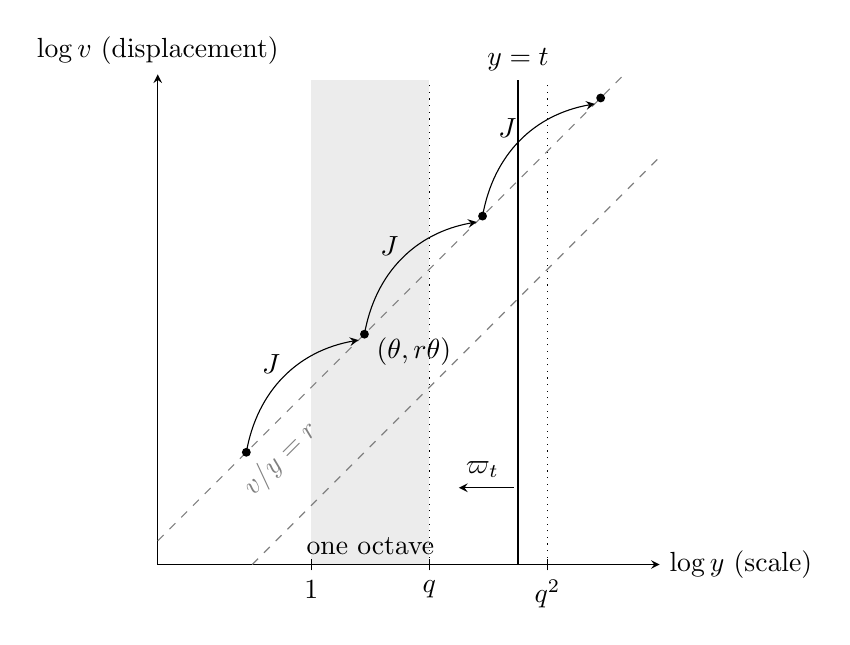
\begin{tikzpicture}[x=1.5cm, y=1.5cm, >=stealth]
  \fill[gray!15] (0,-1.2) rectangle (1,2.9);
  \draw[->] (-1.3,-1.2) -- (2.95,-1.2) node[right] {$\log y$ (scale)};
  \draw[->] (-1.3,-1.2) -- (-1.3,2.95) node[above] {$\log v$ (displacement)};
  \foreach \x/\lab in {0/1, 1/q, 2/q^2} {
    \draw (\x,-1.25) -- (\x,-1.15);
    \node[below] at (\x,-1.25) {$\lab$};
  }
  \draw[dotted] (1,-1.2) -- (1,2.9);
  \draw[dotted] (2,-1.2) -- (2,2.9);
  \node[above] at (0.5,-1.2) {one octave};
  \draw[dashed, gray] (-1.3,-1.0) -- node[pos=0.22, sloped, below=2pt] {$v/y = r$} (2.65,2.95);
  \draw[dashed, gray] (-0.5,-1.2) -- (2.95,2.25);
  \foreach \n in {-1,0,1,2} {
    \fill (0.45+\n,0.75+\n) circle (1.6pt);
  }
  \foreach \n in {-1,0,1} {
    \draw[->, bend left=35] (0.45+\n,0.75+\n) to node[above left, inner sep=1pt] {$J$}
      (1.4+\n,1.7+\n);
  }
  \node[right] at (0.47,0.6) {$(\theta, r\theta)$};
  \draw[thick] (1.75,-1.2) -- (1.75,2.9);
  \node[above] at (1.75,2.9) {$y = t$};
  \draw[<-] (1.25,-0.55) -- (1.72,-0.55);
  \node[above] at (1.45,-0.55) {$\varpi_t$};
\end{tikzpicture}
\caption{The quadrant of scales $y$ and displacements $v$, both axes logarithmic. The dilation
$J(y,v) = (qy, qv)$ moves a point one octave along a diagonal, a line of constant ratio $r = v/y$.
One orbit of $J$ (the dots) carries a knot-atom cascade, which at the knot $\theta q^n$ jumps by
$\pm r\theta q^n$ (Theorem~\ref{thm:knot-atom-cascades}). The shaded octave $1 \le y < q$ meets
each orbit once, so a $J$-invariant measure is fixed by its restriction there. The \Levy{} measure
$\varpi_t$ of the family is the mass of $\Lambda$ to the left of the line $y = t$
(Theorem~\ref{thm:surface-measure}).}
\label{fig:quadrant}
\end{figure}

% shared with blueprint lem:averaging-bound
\begin{lemma}[the averaging bound]
\label{lem:averaging-bound}

\begin{enumerate}
\item For real $v$, $1 \wedge v^2 \le 3(1 - \cos v) + \int_0^2(1 - \cos\omega v)\,d\omega$.
\item If $\psi \in \mathrm{ND}_s$ has the data $(\alpha, \rho)$, then $\alpha \le \psi(1)$ and
\[
  \int(1 \wedge v^2)\,\rho(dv) \ \le\ 3\psi(1) + \int_0^2\psi(\omega)\,d\omega .
\]
\item If $\psi \in \mathrm{ND}_s$, and a measure $\rho$ on $\RR$ that is a countable sum of finite
measures has $\int(1 - \cos\omega v)\,\rho(dv) \le \psi(\omega)$ for every real $\omega$, then
$\int(1 \wedge v^2)\,\rho(dv) < \infty$.
\end{enumerate}
\end{lemma}

\begin{proof}
(1) For $|v| \le 1$, $v^2 \le 3(1 - \cos v)$, by the Taylor bound of $\cos$, and the integral is
nonnegative. For $|v| \ge 1$ the integral is $2 - \sin(2v)/v \ge 1 \ge 1 \wedge v^2$.

(2) $\alpha = \alpha\cdot1^2 \le \psi(1)$. Integrate (1) against $\rho$. By Tonelli's theorem,
\[
  \int(1 \wedge v^2)\,\rho(dv) \le 3\int(1 - \cos v)\,\rho(dv)
  + \int_0^2\int(1 - \cos\omega v)\,\rho(dv)\,d\omega ,
\]
and $\int(1 - \cos\omega v)\,\rho(dv) \le \psi(\omega)$ for every $\omega$, the Gaussian term being
nonnegative.

(3) The same computation applies, Tonelli's theorem holding for a countable sum of finite measures,
and gives $\int(1 \wedge v^2)\,\rho(dv) \le 3\psi(1) + \int_0^2\psi(\omega)\,d\omega$. The right side
is finite. If $\psi$ has the data $(a, \varpi)$, then for $0 < \omega \le 2$ one has
$1 - \cos\omega v \le 2(1 \wedge v^2)$, so $\psi(\omega) \le 4a + 2\int(1 \wedge v^2)\,\varpi(dv)$.

Every step is machine-checked, with no cited fact.
\end{proof}

% shared with blueprint thm:surface-measure
\begin{theorem}[the surface measure]
\label{thm:surface-measure}

Let $J(y,v) := (qy, qv)$ on $(0,\infty)^2_{(y,v)}$. In the canonical discrete gauge, the
$q^{\ZZ}$-covariant families are in bijection with the pairs $(\Lambda, \mathcal{B})$ of a positive
measure $\Lambda$ on $(0,\infty)^2$ and a positive measure $\mathcal{B}$ on $(0,\infty)_y$ such that
\begin{enumerate}
\item[(i)] $J_*\Lambda = \Lambda$, and $\int(1 \wedge v^2)\,\Lambda((0,t] \times dv) < \infty$ for
some, equivalently every, $t > 0$;
\item[(ii)] $\mathcal{B}((0,t]) < \infty$ for $t > 0$, and $\mathcal{B}(qA) = q^2\mathcal{B}(A)$ for
Borel $A \subseteq (0,\infty)$;
\item[(iii)] $\Lambda(\{y\} \times (0,\infty)) = 0$ and $\mathcal{B}(\{y\}) = 0$ for every $y > 0$;
\item[(iv)] $\Lambda((s,t] \times (0,\infty)) + \mathcal{B}((s,t]) > 0$ for $0 < s < t$;
\end{enumerate}
the family being given by
\begin{equation}\label{eq:line-e1}
  \varpi_t = \Lambda\bigl((0,t] \times \cdot\,\bigr), \qquad a(t) = \mathcal{B}\bigl((0,t]\bigr),
\end{equation}
equivalently
\begin{equation}\label{eq:line-e2}
  \Psi_t(\omega) = a(t)\,\omega^2 + \int_{(0,t] \times (0,\infty)}\bigl(1 - \cos\omega v\bigr)\,
  \Lambda(dy, dv).
\end{equation}
\end{theorem}

\begin{proof}
\emph{From a family to $(\Lambda, \mathcal{B})$: the data.} Let the kernels have the data
$(a(t), \varpi_t)$, $t \ge 0$, so that $(a(0), \varpi_0) = (0, 0)$, as $\mu_0 = \delta_0$. For
$s < t$ the step $\mu_{s,t}$ is symmetric and infinitely divisible
(Lemma~\ref{lem:family-structure}) with the exponent $\Psi_t - \Psi_s$, by (I1); so
$\Psi_t - \Psi_s \in \mathrm{ND}_s$, and by Lemma~\ref{lem:line-exponent-data}(3)
$a(s) \le a(t)$, $\varpi_s \le \varpi_t$, and $\Psi_t - \Psi_s$ has the data
$(a(t) - a(s), \varpi_t - \varpi_s)$. Covariance at the pairs $(0, t)$ gives
$\Psi_{qt} = \Psi_t(q\,\cdot)$, so $(a(qt), \varpi_{qt}) = (q^2a(t), T_q\varpi_t)$ by
Lemma~\ref{lem:line-exponent-data}(1),(2). Put
$G(t) := 3\Psi_t(1) + \int_0^2\Psi_t(\omega)\,d\omega$. The averaging bound,
Lemma~\ref{lem:averaging-bound}(2), for $\Psi_t - \Psi_s$ gives
\[
  a(t) - a(s) \le \Psi_t(1) - \Psi_s(1), \qquad
  (1 \wedge \varepsilon^2)\,(\varpi_t(A) - \varpi_s(A)) \le G(t) - G(s)
\]
for every Borel $A \subseteq (\varepsilon, \infty)$, $\varepsilon > 0$. By (I2) and
$\widehat\mu_t > 0$, $t \mapsto \Psi_t(\omega)$ is continuous on $[0,\infty)$; and
$0 \le \Psi_t \le \Psi_T$ for $t \le T$ with $\Psi_T$ continuous, so $G$ is continuous by
dominated convergence. Hence $a$ is continuous and nondecreasing, and so is $t \mapsto \varpi_t(A)$
for every Borel $A$ bounded away from $0$.

\emph{The measure $\Lambda$.} Fix $T > 0$ and put $W := \varpi_T$, a measure on $(0,\infty)$
finite on every $(\varepsilon,\infty)$, hence $\sigma$-finite. For rational $r$ let
$h_r := 1 \wedge d\varpi_r/dW$ when $0 < r < T$, $h_r := 0$ when $r \le 0$ and $h_r := 1$ when
$r \ge T$. Then $\int_A h_r\,dW = \varpi_{r \wedge T}(A)$ for Borel $A$, since
$d\varpi_r/dW \le 1$ $W$-a.e., and for rationals $r' \le r$ we have $h_{r'} \le h_r$ $W$-a.e., as
$\varpi_{r'} \le \varpi_r$. Put $f_r(v) := \sup_{r' \le r}h_{r'}(v)$ and
$F_r(v) := \inf_{r' > r}f_{r'}(v)$, over rationals. Then $f_r = h_r$ $W$-a.e., and for every $v$
the function $r \mapsto F_r(v)$ is nondecreasing and right-continuous on the rationals, vanishes for
$r < 0$ and equals $1$ for $r \ge T$. So it extends to a distribution function on $\RR$, whose
law $\kappa_v$ depends measurably on $v$, with $\kappa_v((-\infty, t]) = \inf_{r > t}f_r(v)$. For
Borel $A \subseteq (\varepsilon,\infty)$ and $t \ge 0$, monotone convergence (the $f_r$ are at most
$1$ and $W(A) < \infty$) and the right-continuity of $t \mapsto \varpi_t(A)$ give
\[
  \int_A\kappa_v\bigl((-\infty, t]\bigr)\,W(dv) = \inf_{r > t}\int_A f_r\,dW
  = \inf_{r > t}\varpi_{r \wedge T}(A) = \varpi_{t \wedge T}(A).
\]
Let $\Lambda_T$ be the image of the measure $W(dv)\,\kappa_v(dy)$ under $(v, y) \mapsto (y, v)$. At
$t = 0$ the display gives $\Lambda_T((-\infty,0] \times (\varepsilon,\infty)) = 0$, and
$\Lambda_T(\RR \times (-\infty, 0]) = W((-\infty,0]) = 0$, so $\Lambda_T$ is carried by
$(0,\infty)^2$; and $\Lambda_T((0,t] \times A) = \varpi_{t \wedge T}(A)$ for $t > 0$. Two measures
on $(0,\infty)$ that agree on the Borel sets bounded away from $0$ are equal, so
$\Lambda_T((0,t] \times \cdot\,) = \varpi_{t \wedge T}$.

\emph{Uniqueness on the quadrant.} Two measures $\Lambda, \Lambda'$ on $(0,\infty)^2$ with the
same slabs $\Lambda((0,t] \times \cdot\,)$, finite on every $(\varepsilon,\infty)$, are equal.
Indeed, for Borel $A \subseteq (\varepsilon,\infty)$ the measures $S \mapsto \Lambda(S \times A)$
and $S \mapsto \Lambda'(S \times A)$ on $(0,\infty)$ agree, finitely, on the intervals $(0,t]$,
hence on all Borel sets. The products $S \times A$ with
$A \subseteq (-\infty,0] \cup (\varepsilon,\infty)$ for some $\varepsilon > 0$ form a
$\pi$-system that generates the Borel sets of $\RR^2$; both measures agree on them, and countably
many of them, the sets $(-n,n] \times ((-\infty,0] \cup (1/(n+1),\infty))$, have finite measure
and cover $\RR^2$. So $\Lambda = \Lambda'$. In particular, for $m \le n$ the restriction of
$\Lambda_{n+1}$ to $(0, m+1] \times \RR$ is $\Lambda_{m+1}$, and
$\Lambda := \sum_{n \ge 0}\Lambda_{n+1}|_{(n, n+1] \times \RR}$ has
$\Lambda((0,t] \times \cdot\,) = \varpi_t$ for every $t > 0$.

Let $\mathcal{B}$ be the Stieltjes measure of the continuous nondecreasing function
$t \mapsto a(t \vee 0)$. Then $a(t) = \mathcal{B}((0,t])$ and $\mathcal{B}((-\infty,0]) = 0$.
This is (\ref{eq:line-e1}), and (\ref{eq:line-e2}) follows by substituting. Any $\Lambda'$ on $(0,\infty)^2$ and
$\mathcal{B}'$ on $(0,\infty)$ with (\ref{eq:line-e1}) have the slabs $\Lambda'((0,t] \times \cdot\,)$ and the
masses $\mathcal{B}'((0,t])$ of the data of $\mu_t$, which are unique
(Lemma~\ref{lem:line-exponent-data}(1)). So $\Lambda' = \Lambda$ by the uniqueness on the
quadrant, and $\mathcal{B}' = \mathcal{B}$, two measures on $(0,\infty)$ that agree, finitely, on
every $(0,t]$ being equal.

(i) $J^{-1}((0,t] \times A) = (0,t/q] \times q^{-1}A$, so the slabs of $J_*\Lambda$ are
$T_q\varpi_{t/q} = \varpi_t$, and $J_*\Lambda = \Lambda$ by the uniqueness on the quadrant.
Integrability at every $t$ holds because $\varpi_t$ is a \Levy{} measure. For a general invariant
$\Lambda$,
\[
  \int(1 \wedge v^2)\,\Lambda((0,qt] \times dv) = \int(1 \wedge q^2v^2)\,\Lambda((0,t] \times dv)
  \le q^2\int(1 \wedge v^2)\,\Lambda((0,t] \times dv),
\]
and the integral is nondecreasing in $t$. So integrability at one $t$ gives it at all.
(ii) The measures $A \mapsto \mathcal{B}(qA)$ and $q^2\mathcal{B}$ on $(0,\infty)$ agree, finitely,
on the intervals $(0,t]$, since $a(qt) = q^2a(t)$, hence on all Borel sets.
(iii) For $0 < s < y$ and $\varepsilon > 0$,
$\Lambda(\{y\} \times (\varepsilon,\infty)) \le \Lambda((s,y] \times (\varepsilon,\infty))
= \varpi_y((\varepsilon,\infty)) - \varpi_s((\varepsilon,\infty))
\le (G(y) - G(s))/(1 \wedge \varepsilon^2)$, which tends to $0$ as $s \uparrow y$. So
$\Lambda(\{y\} \times (\varepsilon,\infty)) = 0$ for every $\varepsilon > 0$, and
$\Lambda(\{y\} \times (0,\infty)) = 0$. $\mathcal{B}$ has no atoms because $a$ is continuous.
(iv) If $\Lambda((s,t] \times (0,\infty)) = 0 = \mathcal{B}((s,t])$, then $a(t) = a(s)$ and
$\varpi_t = \varpi_s$, the data of $\mu_{s,t}$ vanish, and $\mu_{s,t} = \delta_0$, against (ND).

\emph{From $(\Lambda, \mathcal{B})$ to a family.} Given a pair with (i)--(iv), define $a(t)$ and
$\varpi_t$ by (\ref{eq:line-e1}). By (i), $\varpi_t$ is a \Levy{} measure on $(0,\infty)$, and $\Psi_t$ given
by (\ref{eq:line-e2}) lies in $\mathrm{ND}_s$ with the data $(a(t), \varpi_t)$. For $0 \le s < t$,
$\Psi_t \ne \Psi_s$: otherwise their data agree (Lemma~\ref{lem:line-exponent-data}(1)), so
$\mathcal{B}((s,t]) = 0$ and $\Lambda((s,t] \times (\varepsilon,\infty)) = 0$ for every
$\varepsilon > 0$, the masses being finite, and (iv) fails on $(s \vee t/2, t]$. With $s = 0$, where
$\Psi_0 = 0$, this gives $\Psi_t \not\equiv 0$. For $t < t'$ in $[1,q]$ the data are ordered,
$a(t) \le a(t')$ and $\varpi_t \le \varpi_{t'}$, so condition (2) of
Theorem~\ref{thm:annulus-parametrization} holds by Lemma~\ref{lem:line-exponent-data}(3).
Gluing: by $J_*\Lambda = \Lambda$ and the change of variables $(y, v) = J(y', v')$,
$\int_{(0,qt] \times (0,\infty)}(1 - \cos\omega v)\,\Lambda(dy, dv)
= \int_{(0,t] \times (0,\infty)}(1 - \cos q\omega v')\,\Lambda(dy', dv')$, and
$a(qt) = \mathcal{B}(q(0,t]) = q^2a(t)$ by (ii), so $\Psi_{qt} = \Psi_t(q\,\cdot)$ for every
$t > 0$, in particular $\Psi_q = \Psi_1(q\,\cdot)$. Continuity: on $(0,T] \times (0,\infty)$ the
integrand of (\ref{eq:line-e2}) is integrable, its integral being at most the exponent of the data at $T$; by
(iii) no vertical line carries mass of $\Lambda$, and $\mathcal{B}$ has no atoms. So $a(t)$ and the
integral in (\ref{eq:line-e2}) are continuous in $t$ by dominated convergence, the indicator of $(0,t]$
converging off the line $\{t_0\} \times (0,\infty)$ as $t \to t_0$.
Theorem~\ref{thm:annulus-parametrization} gives a family whose exponents at every $t \ge 0$ are the
path extended by $\Psi_{q^nt} := \Psi_t(q^n\,\cdot)$, which by $\Psi_{qt} = \Psi_t(q\,\cdot)$ is
(\ref{eq:line-e2}) itself. So its kernels have the data (\ref{eq:line-e1}), and its pair, constructed in the first part, is
$(\Lambda, \mathcal{B})$ by the uniqueness. The map from families to pairs is injective: two
families with the data (\ref{eq:line-e1}) have the same exponents at every $t > 0$, so their kernels agree on
$[1,q)$ and the families coincide (Lemma~\ref{lem:discrete-covariance-levy}). So the two maps are
inverse bijections. (\ref{eq:line-e1}) and (\ref{eq:line-e2}) are equivalent for a pair with (i)--(iv), since the
exponent of the data in (\ref{eq:line-e1}) is (\ref{eq:line-e2}) and the data of an exponent are unique.

Every step is machine-checked, and the cited facts enter only through the statements the proof
cites.
\end{proof}

% shared with blueprint lem:null-conull-point-mass
\begin{lemma}[a measure with no proper part is a point mass]
\label{lem:null-conull-point-mass}

Let $\kappa$ be a measure on $\RR$ or on $\RR^2$ such that every Borel set $E$ has $\kappa(E) = 0$
or $\kappa(E^c) = 0$. Then $\kappa = \kappa(\{p\})\,\delta_p$ for some point $p$.
\end{lemma}

\begin{proof}
On $\RR$, let $S := \{x : \kappa((x,\infty)) = 0\}$. If $S$ is empty, then
$\kappa((-\infty, n]) = 0$ for every integer $n$, and if $S$ is unbounded below, then
$\kappa((-n,\infty)) = 0$ for every $n$; in both cases $\kappa = 0$ by continuity from below, and
any $p$ will do. Otherwise $\tau := \inf S$ is finite. Every $x > \tau$ lies in $S$, so
$\kappa((\tau,\infty)) = 0$, and every $x < \tau$ lies outside $S$, so $\kappa((-\infty,x]) = 0$ and
$\kappa((-\infty,\tau)) = 0$. So $\kappa$ is carried by $\{\tau\}$, and $\kappa = \kappa(\{\tau\})\,
\delta_\tau$.

On $\RR^2$, the images of $\kappa$ under the two coordinate maps have the same property, so they are
carried by points $\theta$ and $r$. The complement of $\{(\theta, r)\}$ lies in the union of
$(\RR \setminus \{\theta\}) \times \RR$ and $\RR \times (\RR \setminus \{r\})$, both $\kappa$-null,
so $\kappa$ is carried by $(\theta, r)$.

Every step is machine-checked, with no cited fact.
\end{proof}

The next theorem places its atoms on knots of every phase. For a phase $\theta \in [1,q)$ the
scales $\theta q^n$, $n \in \ZZ$, are the \emph{knots of phase $\theta$}. The knots of a family in
the canonical discrete gauge are those of phase $1$.

% shared with blueprint thm:knot-atom-cascades
\begin{theorem}[the knot-atom cascades]
\label{thm:knot-atom-cascades}

For $y > 0$ let $[y] \in [1,q)$ be its representative modulo $q^{\ZZ}$, and let
$\mathcal{C} := [1,q)_\theta \times (0,\infty)_r$, the \emph{cylinder}.
\begin{enumerate}
\item The group $\{J^n : n \in \ZZ\}$ acts freely and properly discontinuously on $(0,\infty)^2$.
The invariant map $(y,v) \mapsto (\log y \operatorname{mod} \ell,\ v/y)$ induces a homeomorphism of the orbit
space onto $(\RR/\ell\ZZ) \times (0,\infty)$, and $[1,q) \times (0,\infty)$ meets every orbit
exactly once. The ratio $r := v/y$ is the invariant \emph{displacement-to-scale ratio}.
\item Let $\sigma$ be the image of the restriction of $\Lambda$ to $[1,q) \times (0,\infty)$ under
$(y,v) \mapsto (y, v/y)$. Then $\Lambda \mapsto \sigma$ is a bijection of the $J$-invariant positive
measures on $(0,\infty)^2$ onto the positive measures on $\mathcal{C}$, with inverse
\[
  \sigma \mapsto \Lambda_\sigma := \int_{\mathcal{C}}\Lambda^{(\theta,r)}\,\sigma(d\theta,dr),
  \qquad \Lambda^{(\theta,r)} := \sum_{n \in \ZZ}\delta_{(\theta q^n,\, r\theta q^n)} .
\]
$\Lambda_\sigma$ satisfies the integrability of Theorem~\ref{thm:surface-measure}(i) iff
\begin{equation}\label{eq:line-e3}
  \int_{\mathcal{C}}\Bigl[(r\theta)^2 \wedge \bigl(1 + \log_+(r\theta)\bigr)\Bigr]\,
  \sigma(d\theta,dr) < \infty ,
\end{equation}
and it has no mass on a line $\{y\} \times (0,\infty)$ iff
$\sigma(\{\theta\} \times (0,\infty)) = 0$ for every $\theta$. Likewise $\mathcal{B}$ with
Theorem~\ref{thm:surface-measure}(ii) corresponds to its restriction $\beta$ to $[1,q)$, by
$\mathcal{B}(A) = \sum_nq^{2n}\beta(q^{-n}A \cap [1,q))$.
\item The extreme rays of the cone of $J$-invariant $\Lambda$ with the integrability (\ref{eq:line-e3}) are the
rays of the $\Lambda^{(\theta,r)}$, $(\theta,r) \in \mathcal{C}$, and every such $\Lambda$ is the
mixture $\Lambda_\sigma$ with $\sigma$ unique. With $\mathcal{B} = 0$, the exponents (\ref{eq:line-e2}) of
$\Lambda^{(\theta,r)}$ are the \emph{knot-atom cascade}
\begin{equation}\label{eq:line-e4}
  \Psi^{(\theta,r)}_t(\omega) = \sum_{n :\ \theta q^n \le t}\bigl(1 - \cos(\omega\,r\theta q^n)\bigr).
\end{equation}
The extreme rays of the cone of the $\mathcal{B}$ are those of
$\mathcal{B}^{(\theta)} := \sum_n(\theta q^n)^2\delta_{\theta q^n}$, the \emph{knot Gaussians}
$a(t) = \sum_{n :\ \theta q^n \le t}(\theta q^n)^2$.
\item A knot-atom cascade is constant in $t$ between consecutive knots $\theta q^n$ of phase
$\theta$, and at each of them its kernel is convolved with the law of transform
$e^{-(1 - \cos(r\theta q^n\omega))}$, the compound Poisson law of unit rate with jumps
$\pm r\theta q^n$. It violates (I2), so it is a member of the cone and not a family. A knot
Gaussian jumps by $(\theta q^n)^2$ at each knot $\theta q^n$, so its $\mathcal{B}^{(\theta)}$ has
atoms, against Theorem~\ref{thm:surface-measure}(iii), and it is not a family either. The families
are the pairs $(\Lambda_\sigma, \mathcal{B})$ with (\ref{eq:line-e3}), with $\sigma(\{\theta\} \times (0,\infty)) = 0$
for every $\theta$, $\beta$ without atoms, and Theorem~\ref{thm:surface-measure}(iv).
\end{enumerate}
\end{theorem}

\begin{proof}
(1) $J^n(y,v) = (y,v)$ forces $q^ny = y$, so $n = 0$: the action is free. For a compact
$K \subset (0,\infty)^2$ with $y$-coordinates in $[y_1, y_2]$, $J^nK \cap K \ne \varnothing$ needs
$q^n \in [y_1/y_2, y_2/y_1]$, which holds for finitely many $n$. The map
$p(y,v) := (\log y \operatorname{mod} \ell, v/y)$ is continuous and invariant. It is the map
$\phi(y,v) := (\log y, v/y)$ followed by the quotient map $\RR \to \RR/\ell\ZZ$ on the first
coordinate. The map $\phi$ is a homeomorphism of $(0,\infty)^2$ onto $\RR \times (0,\infty)$, with
inverse $(u, r) \mapsto (e^u, re^u)$, and the quotient map of a topological group is open. So $p$
is open, and it is onto $(\RR/\ell\ZZ) \times (0,\infty)$. Two points with the same image have
$\log y' - \log y \in \ell\ZZ$, that is $y' = q^ny$, and $v'/y' = v/y$, so they lie in one orbit.
A continuous open surjection whose fibres are the orbits induces a homeomorphism of the orbit space.
Each orbit $\{(q^ny, q^nv)\}$ has exactly one $n$ with $q^ny \in [1,q)$, namely
$n = -\lfloor\log_qy\rfloor$.

(2) Write $F := [1,q) \times (0,\infty)$. The sets $J^nF$, $n \in \ZZ$, partition $(0,\infty)^2$, so
an invariant $\Lambda$ satisfies $\Lambda(E) = \sum_n\Lambda(J^{-n}E \cap F)$ and is determined by
its restriction to $F$. Conversely, for any measure on $F$ that sum defines an invariant measure.
Transporting $F$ to $\mathcal{C}$ by $(y,v) \mapsto (y, v/y)$ gives the bijection. Restricted to $F$,
$\Lambda^{(\theta,r)}$ is the single atom at $(\theta, r\theta)$, since only $n = 0$ has
$\theta q^n \in [1,q)$. So the restriction of $\Lambda_\sigma$ to $F$ is the transport of $\sigma$,
and $\Lambda_\sigma$ is the inverse image.

For the integrability, by Tonelli and Theorem~\ref{thm:surface-measure}(i) at $t = 1$,
\[
  \int(1 \wedge v^2)\,\Lambda_\sigma((0,1] \times dv)
  = \int_{\mathcal{C}}\Bigl[f(r\theta) + \mathbf 1_{\{\theta = 1\}}\bigl(1 \wedge (r\theta)^2\bigr)\Bigr]
  \sigma(d\theta,dr), \qquad f(x) := \sum_{m \ge 1}\bigl(1 \wedge x^2q^{-2m}\bigr),
\]
because $\theta q^n \le 1$ means $n \le -1$, or $n \le 0$ when $\theta = 1$. Write
$\Theta(x) := x^2 \wedge (1 + \log_+x)$, and note $\log_+x \le \Theta(x)$ and $1 \wedge x^2 \le \Theta(x)$ for
$x \ge 0$ (as $\log x \le x - 1 \le x^2$). On the one side, the terms of $f$ with $q^m \le x$ number
at most $\log_+x/\ell$, and the others are at most $(1 \wedge x^2)q^{-2j}$, $j \ge 0$, so
$f(x) \le \log_+x/\ell + \tfrac{q^2}{q^2 - 1}(1 \wedge x^2) \le C_q\Theta(x)$ with
$C_q := 1/\ell + q^2/(q^2 - 1)$. On the other side, for $x \le q$ the term $m = 1$ gives
$f(x) \ge x^2/q^2$, so $\Theta(x) \le x^2 \le q^2f(x)$. For $x > q$ the term $m = 1$ is $1$, so
$f(x) \ge 1$, and the terms equal to $1$ number $\lfloor\log_qx\rfloor$, so
$\log x \le \ell(f(x) + 1) \le 2\ell f(x)$ and $\Theta(x) \le 1 + \log x \le (1 + 2\ell)f(x)$. So the
integral is finite iff (\ref{eq:line-e3}) holds, and then it is finite at every $t > 0$ by
Theorem~\ref{thm:surface-measure}(i), $\Lambda_\sigma$ being invariant. A line
$\{y\} \times (0,\infty)$ meets the orbit of $(\theta, r)$ only if $\theta = q^{-n}y$ for some $n$,
so its mass under $\Lambda_\sigma$ is $\sum_n\sigma(\{q^{-n}y\} \times (0,\infty))$, and conversely
$\sigma(\{\theta\} \times (0,\infty))$ is at most the mass of the line $\{\theta\} \times (0,\infty)$,
the term $n = 0$. The statement on $\mathcal{B}$ is the same argument for the action $y \mapsto qy$
with the weight $q^2$: the condition $\mathcal{B}(qA) = q^2\mathcal{B}(A)$ gives
$q^{2n}\mathcal{B}(q^{-n}A) = \mathcal{B}(A)$ for every $n \in \ZZ$, the intervals
$q^n[1,q)$ partition $(0,\infty)$, and for $\beta$ finite on $[1,q)$ the sum
$\sum_nq^{2n}\beta(q^{-n}(0,t] \cap [1,q))$ has no terms with $q^n > t$ and a geometric tail.

(3) By (2) the map $\sigma \mapsto \Lambda_\sigma$ is a bijection, additive and positively
homogeneous, with inverse $\Lambda \mapsto \sigma$, also additive and positively homogeneous. So
$\Lambda = \Lambda_\sigma$ with $\sigma$ unique, and a decomposition $\Lambda = \Lambda' + \Lambda''$
in the cone is the decomposition $\sigma = \sigma' + \sigma''$ of the cylinder measures, each with
(\ref{eq:line-e3}). Let $\Lambda_\sigma$ span an extreme ray, and let $E \subset \mathcal{C}$ be Borel. Then
$\sigma = \sigma|_E + \sigma|_{E^c}$, both terms satisfy (\ref{eq:line-e3}), and extremality gives
$\sigma|_E = c\sigma$ for some $c \ge 0$. Evaluated on $E^c$ this is $0 = c\,\sigma(E^c)$, so either
$\sigma(E^c) = 0$, or $c = 0$ and $\sigma(E) = 0$: every Borel set is $\sigma$-null or
$\sigma$-conull. By Lemma~\ref{lem:null-conull-point-mass}, $\sigma = c\,\delta_{(\theta,r)}$ with
$c = \sigma(\{(\theta,r)\})$ for a point $(\theta, r)$, and $c > 0$ as $\sigma \ne 0$. The point
lies in $\mathcal{C}$, and $c < \infty$ by (\ref{eq:line-e3}), the weight $\Theta(r\theta)$ being positive. So
$\Lambda = c\,\Lambda^{(\theta,r)}$. Conversely, $c\,\delta_{(\theta,r)}$ with $0 < c < \infty$
satisfies (\ref{eq:line-e3}), and in a decomposition $c\,\delta_{(\theta,r)} = \sigma' + \sigma''$ the measure
$\sigma'$ vanishes off $(\theta, r)$, so it is a multiple $c'\delta_{(\theta,r)}$, $c' \le c$, and
$\Lambda_{\sigma'} = (c'/c)\,c\Lambda^{(\theta,r)}$. Inserting $\Lambda^{(\theta,r)}$ in (\ref{eq:line-e2}), the
integral over $(0,t] \times (0,\infty)$ is the sum over the atoms $(\theta q^n, r\theta q^n)$ with
$\theta q^n \le t$, which is (\ref{eq:line-e4}). The sum converges, since its terms vanish for $\theta q^n > t$
and are at most $\tfrac12(\omega r\theta)^2q^{2n}$, by $1 - \cos u \le u^2/2$. For $\mathcal{B}$ the
same argument applies to $\beta$, on $\RR$, where $\beta$ is finite. The point mass at $\theta$
gives $\sum_nq^{2n}\delta_{\theta q^n}$, which is $\theta^{-2}\mathcal{B}^{(\theta)}$, and
$\mathcal{B}^{(\theta)}((0,t])$ is the sum of the atoms $(\theta q^n)^2$ with $\theta q^n \le t$.

(4) For $t \in [\theta q^n, \theta q^{n+1})$, $\theta q^m \le t$ holds iff $m \le n$. So the sum
(\ref{eq:line-e4}) is constant on $[\theta q^n, \theta q^{n+1})$, and from $t \in [\theta q^{n-1}, \theta q^n)$
to $\theta q^n$ it gains exactly the term $m = n$, $1 - \cos(\omega r\theta q^n)$. That function is
the exponent of the compound Poisson law
$\exp[\delta^2_v] = e^{-1}\sum_{k \ge 0}(\tfrac12(\delta_v + \delta_{-v}))^{*k}/k!$, $v = r\theta q^n$:
the step $\tfrac12(\delta_v + \delta_{-v})$ has the transform $\cos v\omega$, so the law has the
transform $e^{-1}\sum_k(\cos v\omega)^k/k! = e^{-(1 - \cos v\omega)}$. The transforms multiply, so
the kernel at $\theta q^n$ is the kernel at $t$ convolved with $\exp[\delta^2_v]$, the transform
determining the law. The cascade violates (I2): if a family of laws $\mu_{s,t}$ with (I1), (I2) had
$\widehat{\mu_{0,t}} = e^{-\Psi^{(\theta,r)}_t}$, then at $\omega = \pi/(r\theta)$ the function
$t \mapsto \widehat{\mu_{0,t}}(\omega)$ would be continuous at $t = \theta$; it is constant on
$[\theta/q, \theta)$, and at $\theta$ the exponent gains $1 - \cos\pi = 2$, so the value there differs
from the limit from the left. The knot Gaussian $a(t) = \sum_{\theta q^n \le t}(\theta q^n)^2$
jumps by $(\theta q^n)^2$ at $\theta q^n$, since the points $\theta q^m$ are distinct, so
$\mathcal{B}^{(\theta)}(\{\theta q^n\}) > 0$, against Theorem~\ref{thm:surface-measure}(iii): no pair
with (i)--(iv) has this $\mathcal{B}$. The description of the families is (i)--(iv) read through
(2): $\Lambda_\sigma$ is invariant and carried by $(0,\infty)^2$, its integrability is (\ref{eq:line-e3}), and it
has no mass on a vertical line iff $\sigma(\{\theta\} \times (0,\infty)) = 0$ for every $\theta$;
$\mathcal{B}$ has no atoms iff $\beta$ has none, since
$\mathcal{B}(\{y\}) = \sum_nq^{2n}\beta(\{q^{-n}y\})$ and an atom of $\beta$ at $y \in [1,q)$ is an
atom of $\mathcal{B}$.

Every step is machine-checked, with no cited fact.
\end{proof}

In the generator form (\ref{eq:generator-form}), with the symmetric second difference
$\delta^2_h$ defined there, a knot-atom cascade jumps at each of its knots by the compound Poisson
law $\exp[\delta^2_{r\theta q^n}]$, whose generator is the second difference $\delta^2_{r\theta q^n}$,
and does nothing between them. The generator of a Cin ray is a single symmetric second
difference at every scale \prog{V-cone v0.1}{Prop.~6.4(5), p.~58}.

% shared with blueprint prop:strata-cylinder-coordinates
\begin{proposition}[the strata in cylinder coordinates; circle averaging]
\label{prop:strata-cylinder-coordinates}

Let $\eta(d\theta) := d\theta/(\ell\theta)$ on $[1,q)$, the Haar probability measure of the circle
$(0,\infty)/q^{\ZZ}$. Let a $q^{\ZZ}$-covariant family in the canonical discrete gauge have the pair
$(\Lambda, \mathcal{B})$ of Theorem~\ref{thm:surface-measure}, with
$\varpi_t = \Lambda((0,t] \times \cdot\,)$ and $a(t) = \mathcal{B}((0,t])$, and the cylinder
measures $(\sigma, \beta)$ of Theorem~\ref{thm:knot-atom-cascades}. Write
$J_\lambda(y,v) := (\lambda y, \lambda v)$ for $\lambda > 0$.
\begin{enumerate}
\item (The jump part.) The following are equivalent: (a) $\varpi_{\lambda t} = T_\lambda\varpi_t$
for all $\lambda, t > 0$; (b) $(J_\lambda)_*\Lambda = \Lambda$ for every $\lambda > 0$;
(c) $\sigma = \eta \otimes \tilde\rho$ for a measure $\tilde\rho$ on $(0,\infty)$. Then $\Lambda$ is
the image of $(dy/(\ell y)) \otimes \tilde\rho$ under $(y,r) \mapsto (y, ry)$, and
$\varpi_t(dv) = k(v/t)\,dv/v$ with $k(x) := \ell^{-1}\tilde\rho([x,\infty))$, nonincreasing. The
integrability (\ref{eq:line-e3}) is equivalent to each of $\int(r^2 \wedge (1 + \log_+r))\,\tilde\rho(dr) < \infty$
and $\int(1 \wedge x^2)\,k(x)\,dx/x < \infty$.

(The Gaussian part.) The following are equivalent: (a$'$) $a(\lambda t) = \lambda^2a(t)$ for all
$\lambda, t > 0$; (b$'$) $\mathcal{B}(\lambda A) = \lambda^2\mathcal{B}(A)$ for all $\lambda > 0$
and Borel $A$; (c$'$) $\beta(d\theta) = b\,\theta\,d\theta$ with $b \ge 0$. Then
$a(t) = \tfrac b2t^2$.

(Both parts.) $\Psi_{\lambda t}(\omega) = \Psi_t(\lambda\omega)$ for all $\lambda, t > 0$ iff
(a) and (a$'$) hold.
\item The circle average of a knot-atom cascade is a Cin ray:
\begin{equation}\label{eq:line-e5}
  \int_{[1,q)}\Psi^{(\theta,r)}_t(\omega)\,\eta(d\theta) = \frac1\ell\,\Cin(\omega\,r\,t).
\end{equation}
\item For a compact $A \subset (0,\infty)$ and $j \in \ZZ$ let
$\widehat\sigma_j(A) := \int_{[1,q) \times A}e^{2\pi ij\log_q\theta}\,\sigma(d\theta,dr)$. The
\emph{modulation spectrum} of the family is the set of $j \ne 0$ with $\widehat\sigma_j \ne 0$. It
is empty iff $\sigma = \eta \otimes \tilde\rho$ for some $\tilde\rho$.
\end{enumerate}
\end{proposition}

\begin{proof}
(1) \emph{The jump part}, (a)$\Leftrightarrow$(b). Fix $\lambda > 0$. For $t > 0$ and Borel $A$,
$\Lambda(J_\lambda^{-1}((0,t] \times A)) = \Lambda((0,t/\lambda] \times \lambda^{-1}A)
= \varpi_{t/\lambda}(\lambda^{-1}A) = (T_\lambda\varpi_{t/\lambda})(A)$. So
$\varpi_{\lambda s} = T_\lambda\varpi_s$ for all $s > 0$ iff $(J_\lambda)_*\Lambda$ and $\Lambda$
agree on the sets $(0,t] \times A$ with $A \subseteq [\varepsilon,\infty)$ Borel, $\varepsilon > 0$.
These sets form a $\pi$-system that generates the Borel sets of $(0,\infty)^2$, both measures are
finite on each of them, and countably many of them cover $(0,\infty)^2$. So this holds iff
$(J_\lambda)_*\Lambda = \Lambda$.

(b)$\Leftrightarrow$(c). By Theorem~\ref{thm:knot-atom-cascades}(2), $\Lambda = \Lambda_\sigma$,
and $\sigma$ satisfies (\ref{eq:line-e3}). For $\lambda > 0$ let $R_\lambda(\theta, r) := ([\lambda\theta], r)$
be the rotation of the cylinder by $\lambda$. \emph{The cylinder measure of
$(J_\lambda)_*\Lambda_\sigma$ is $(R_\lambda)_*\sigma$.} Indeed, of the points
$(\lambda\theta q^n, \lambda r\theta q^n)$, $n \in \ZZ$, of the dilated orbit of
$(\theta, r) \in \mathcal{C}$, exactly one has its first coordinate in $[1,q)$, the one with
$\lambda\theta q^n = [\lambda\theta]$, and its ratio of coordinates is $r$; so its image under
$(y,v) \mapsto (y, v/y)$ is $R_\lambda(\theta, r)$.

\emph{The case $\sigma = \eta \otimes \tilde\rho$.} Let $\tilde\rho$ be a $\sigma$-finite measure
on $(0,\infty)$ (the $\tilde\rho$ of (c) is, by the bound in the paragraph ``From the slices to the
product''), and $G \ge 0$ Borel on $(0,\infty)$. Since $y \mapsto q^ny$ maps $[1,q)$ onto
$[q^n, q^{n+1})$, these intervals partition $(0,\infty)$, and $dy/y$ is invariant under dilations,
\[
  \int_{[1,q)}\sum_{n \in \ZZ}G(\theta q^n)\,\eta(d\theta) = \int_{(0,\infty)}G(y)\,\frac{dy}{\ell y} .
\]
Applied at fixed $r$ to $G(y) = \mathbf 1_E(y, ry)$, with Tonelli, this shows that
$\Lambda_{\eta \otimes \tilde\rho}$ is the image of $(dy/(\ell y)) \otimes \tilde\rho$ under
$(y,r) \mapsto (y, ry)$. Then $J_\lambda$ composed with this map is the map composed with
$(y,r) \mapsto (\lambda y, r)$, and $dy/(\ell y)$ is invariant under $y \mapsto \lambda y$; so
$\Lambda_{\eta \otimes \tilde\rho}$ is invariant under every $J_\lambda$. This gives
(c)$\Rightarrow$(b), and, as $\Lambda = \Lambda_\sigma$, the description of $\Lambda$ in the
statement. It also shows that $\eta$ is invariant under every rotation: for
$\sigma_0 := \eta \otimes \delta_1$, the cylinder measure of $(J_\lambda)_*\Lambda_{\sigma_0}$ is
both $\sigma_0$ and $(R_\lambda)_*\sigma_0$; the first marginal of $\sigma_0$ is $\eta$, and that of
$(R_\lambda)_*\sigma_0$ is the image of $\eta$ under $\theta \mapsto [\lambda\theta]$.

\emph{Rotation-invariant measures on the circle.} For a measure $\nu$ on $[1,q)$ write
$\widehat\nu_j := \int e^{2\pi ij\log_q\theta}\,\nu(d\theta)$, $j \in \ZZ$. Since
$\log_q[\lambda\theta] = \log_q\lambda + \log_q\theta - n$ with $n$ an integer, the image of $\nu$
under $\theta \mapsto [\lambda\theta]$ has the coefficients
$e^{2\pi ij\log_q\lambda}\,\widehat\nu_j$. If $\nu$ is invariant under every rotation, then for
$j \ne 0$ the choice $\lambda = q^{1/(2j)}$ gives $\widehat\nu_j = -\widehat\nu_j$, so
$\widehat\nu_j = 0$; in particular $\widehat\eta_j = 0$ for $j \ne 0$. \emph{A finite measure $\nu$
on $[1,q)$ with $\widehat\nu_j = 0$ for every $j \ne 0$ is $\nu([1,q))\,\eta$.} The map
$\theta \mapsto \log_q\theta \operatorname{mod} 1$ carries $[1,q)$ bijectively onto $\RR/\ZZ$,
with the measurable inverse $u \mapsto q^u$, $u \in [0,1)$, and it carries $\widehat\nu_j$ to the $j$-th
Fourier coefficient of the image of $\nu$. The images of $\nu$ and of $\nu([1,q))\,\eta$ are finite
measures on $\RR/\ZZ$ with the same Fourier coefficients, by $\widehat\eta_j = 0$ for $j \ne 0$
and $\widehat\eta_0 = 1$. The trigonometric polynomials are dense in the continuous functions on
$\RR/\ZZ$ for the supremum norm, and the integral against a finite measure is continuous in that
norm, so the two images have the same integral against every continuous function; a finite Borel
measure on a metric space is determined by these integrals. So the images agree, and, the map being
injective on $[1,q)$ with a measurable inverse, so do $\nu$ and $\nu([1,q))\,\eta$.

\emph{From the slices to the product.} Let $\tilde\rho(A) := \sigma([1,q) \times A)$. For
$\varepsilon > 0$ the weight of (\ref{eq:line-e3}) is at least $\Theta(\varepsilon) > 0$ on
$[1,q) \times [\varepsilon,\infty)$, with $\Theta(x) := x^2 \wedge (1 + \log_+x)$ nondecreasing, so
$\tilde\rho([\varepsilon,\infty)) < \infty$; and $\tilde\rho$ is null on $(-\infty,0]$, hence
$\sigma$-finite. For a compact $A \subset (0,\infty)$, say $A \subseteq [\varepsilon,\infty)$,
the slice $\sigma_A := \sigma(\cdot \times A)$ is thus a finite measure on $[1,q)$. Suppose that
$\widehat{(\sigma_A)}_j = 0$ for every such $A$ and every $j \ne 0$. Then
$\sigma_A = \tilde\rho(A)\,\eta$, that is $\sigma(E \times A) = \eta(E)\,\tilde\rho(A)$ for Borel
$E$. For fixed $E$ both sides are measures in $A$, null on $(-\infty,0]$, finite on every
$[\varepsilon,\infty)$, and equal on every $[a,b]$ with $a > 0$. Restricted to $[\varepsilon,\infty)$
they are finite measures that agree on the closed intervals, hence equal; letting
$\varepsilon \downarrow 0$, they agree on every Borel $A$. So $\sigma$ and $\eta \otimes \tilde\rho$
agree on the rectangles, and since $\eta$ and $\tilde\rho$ are $\sigma$-finite,
$\sigma = \eta \otimes \tilde\rho$.

(b)$\Rightarrow$(c). Assume (b). Then
$(R_\lambda)_*\sigma = \sigma$ for every $\lambda > 0$, as the cylinder measure of
$(J_\lambda)_*\Lambda = \Lambda$. Since $R_\lambda$ does not move $r$, every slice $\sigma_A$ is
invariant under every rotation, so $\widehat{(\sigma_A)}_j = 0$ for $j \ne 0$, and
$\sigma = \eta \otimes \tilde\rho$.

\emph{The Gaussian part.} (a$'$)$\Leftrightarrow$(b$'$): $a(\lambda t) = \lambda^2a(t)$ is
$\mathcal{B}(\lambda A) = \lambda^2\mathcal{B}(A)$ on the intervals $A = (0,t]$, and two measures
finite on these intervals that agree on them agree on all Borel sets. (a$'$)$\Rightarrow$(c$'$):
$a(t) = a(1)t^2$, so $\mathcal{B}(dy) = 2a(1)\,y\,dy$ and $\beta(d\theta) = b\,\theta\,d\theta$
with $b = 2a(1)$. (c$'$)$\Rightarrow$(b$'$): if $\beta = b\theta\,d\theta$, then
$\mathcal{B} = b\,y\,dy$ by Theorem~\ref{thm:knot-atom-cascades}(2), which is
$\lambda^2$-homogeneous, and $a(t) = \tfrac b2t^2$.

\emph{Both parts.} By Theorem~\ref{thm:surface-measure}, $\Psi_t$ has the data $(a(t), \varpi_t)$.
By Lemma~\ref{lem:line-exponent-data}(1),(2), $\Psi_{\lambda t} = \Psi_t(\lambda\,\cdot)$ iff
$a(\lambda t) = \lambda^2a(t)$ and $\varpi_{\lambda t} = T_\lambda\varpi_t$.

\emph{The profile.} With $\Lambda$ the image of $(dy/(\ell y)) \otimes \tilde\rho$ under
$(y,r) \mapsto (y, ry)$ and the substitution $v = ry$ at fixed $r$, for which $dy/y = dv/v$,
\[
  \varpi_t(A) = \frac1\ell\int\tilde\rho(dr)\int\mathbf 1_{\{y \le t\}}\mathbf 1_A(ry)\,\frac{dy}{y}
  = \int_A\frac1\ell\,\tilde\rho\bigl([v/t, \infty)\bigr)\,\frac{dv}{v}.
\]
By Tonelli, $\int(1 \wedge x^2)k(x)\,dx/x = \ell^{-1}\int g(r)\,\tilde\rho(dr)$ with
$g(r) := \int_0^r(1 \wedge x^2)\,dx/x$, which is $r^2/2$ for $r \le 1$ and $\tfrac12 + \log r$ for
$r > 1$. So $\tfrac12\Theta(r) \le g(r) \le \Theta(r)$ with $\Theta(r) := r^2 \wedge (1 + \log_+r)$. Finally, for
$\theta \in [1,q)$, $\Theta(r) \le \Theta(r\theta) \le \max(q^2, 1 + \ell)\,\Theta(r)$. So (\ref{eq:line-e3}) for
$\eta \otimes \tilde\rho$ is $\int \Theta\,d\tilde\rho < \infty$.
In particular $k$ is finite: $\sigma$ satisfies (\ref{eq:line-e3}) by Theorem~\ref{thm:knot-atom-cascades}(2),
so $\int \Theta\,d\tilde\rho < \infty$, and $\Theta(x)\,\tilde\rho([x,\infty)) \le \int \Theta\,d\tilde\rho$ for
$x > 0$, since $\Theta$ is nondecreasing and positive on $(0,\infty)$. It is nonincreasing because
$x \mapsto \tilde\rho([x,\infty))$ is.

(2) By Tonelli and the substitution $u = \theta q^n$, which maps $[1,q)$ onto $[q^n,q^{n+1})$ with
$du/u = d\theta/\theta$,
\[
  \frac1\ell\int_{[1,q)}\sum_n\mathbf 1_{\{\theta q^n \le t\}}\bigl(1 - \cos(\omega r\theta q^n)\bigr)
  \frac{d\theta}{\theta}
  = \frac1\ell\int_0^t\bigl(1 - \cos(\omega ru)\bigr)\frac{du}{u} = \frac1\ell\,\Cin(\omega rt),
\]
the last step by $\Cin(z) = \int_0^z(1 - \cos v)\,dv/v$ and $v = \omega ru$ for $\omega r > 0$, and
by evenness otherwise.

(3) For compact $A \subset (0,\infty)$, say $A \subseteq [\varepsilon,\infty)$ with
$\varepsilon > 0$, $\sigma([1,q) \times A) \le \tilde\rho([\varepsilon,\infty)) < \infty$, as in (1).
The coefficient $\widehat\sigma_j(A)$ is the coefficient $\widehat{(\sigma_A)}_j$ of the slice
$\sigma_A = \sigma(\cdot \times A)$, since $\sigma$ is carried by $\mathcal{C}$. If the spectrum is
empty, these vanish for every compact $A \subset (0,\infty)$ and every $j \ne 0$, and the paragraph
``From the slices to the product'' of (1) gives $\sigma = \eta \otimes \tilde\rho$. Conversely, if
$\sigma = \eta \otimes \tilde\rho$, then $\widehat\sigma_j(A) = \widehat\eta_j\,\tilde\rho(A) = 0$
for $j \ne 0$, by the rotation invariance of $\eta$.

Every step is machine-checked, and the cited fact enters only through
Lemma~\ref{lem:line-exponent-data}(1).
\end{proof}

Circle averaging connects the two strata. The extreme rays of the cone of the continuous stratum are
the Gaussian ray and the Cin rays \prog{V-cone v0.1}{Prop.~3.3, pp.~15--16}. By (2) the Cin rays
are the circle averages of the knot-atom cascades. The Gaussian ray is the circle average of the
knot Gaussians, since the substitution of the proof of (2) gives
$\int\sum_{\theta q^n \le t}(\theta q^n)^2\,\eta(d\theta) = \ell^{-1}\int_0^tu\,du = t^2/(2\ell)$.
A Cin ray spreads its displacement atoms log-uniformly over the scales, where a knot-atom cascade
switches them on at its knots. In (1) the measure $\ell^{-1}\tilde\rho = -dk$ is the measure
$\kappa^{\mathrm C}$ of (\ref{eq:generator-form}), so at $\sigma = \eta \otimes \tilde\rho$ the
integrability (\ref{eq:line-e3}) is that of (\ref{eq:admissible-exponent}). Full covariance requires both parts
of (1): a Haar cylinder measure $\sigma$ makes the jump part covariant, and the Gaussian part must
in addition satisfy (c$'$).

The next proposition writes each exponent of a semi-selfdecomposable law of span $q$ as a series
over the dilates of one measure $\kappa^{(q)}$, the folded \Levy{} measure of the residual. For laws
this representation is that of Maejima and Ueda: a semi-selfdecomposable law of span $q$ is the law
of $\sum_{j \ge 0}q^{-j}(X_{j+1} - X_j)$ for a \Levy{} process $X$ with a logarithmic moment
[\sscite{maejima2009stochastic}, Thm.~3.3, p.~353, and (3.4), p.~354]. The telescoping in the proof
of the next proposition recurs in Lemmas~\ref{lem:step-field-determines-family}(1) and~\ref{lem:knot-exponent-ladder}(1)
and in Proposition~\ref{prop:extreme-rays-random-walks}(2).

% shared with blueprint prop:strata-cylinder-coordinates-q-cin
\begin{proposition}[the $q$-Cin rays]
\label{prop:strata-cylinder-coordinates-q-cin}

Let $\mathcal{K}_q$ be the set of $\psi \in \mathrm{ND}_s$ whose data $(a, \varpi)$ have
$T_q\varpi \ge \varpi$. For $\tau > 0$ let
\[
  E^{(q)}_\tau(\omega) := \sum_{i \ge 0}\bigl(1 - \cos(\omega\tau q^{-i})\bigr),
\]
the exponent with data $(0, \sum_{i \ge 0}\delta_{\tau q^{-i}})$, the \emph{$q$-Cin ray} of
cutoff $\tau$.
\begin{enumerate}
\item $\mathcal{K}_q$ is a convex cone containing $\omega^2$ and every $E^{(q)}_\tau$. Every
$\psi \in \mathcal{K}_q$ is uniquely
\[
  \psi(\omega) = a\,\omega^2 + \int_{(0,\infty)}E^{(q)}_\tau(\omega)\,\kappa^{(q)}(d\tau)
\]
with $a \ge 0$ and $\kappa^{(q)}$ a positive measure on $(0,\infty)$. A pair $(a, \kappa)$ with
$a \ge 0$ and $\kappa$ a positive measure on $(0,\infty)$ represents in this way an element of
$\mathcal{K}_q$ iff
\[
  \int_{(0,\infty)}\bigl(\tau^2 \wedge (1 + \log_+\tau)\bigr)\,\kappa(d\tau) < \infty .
\]
The extreme rays of $\mathcal{K}_q$ are those of $\omega^2$ and of the $E^{(q)}_\tau$, $\tau > 0$.
\item For $\tau, \omega \in \RR$ with $\tau > 0$,
\[
  \bigl|\ell\,E^{(q)}_\tau(\omega) - \Cin(\tau\omega)\bigr| \le \frac{q\,\ell^2}{2(q - 1)}\,|\tau\omega|,
\]
so $\ell E^{(q)}_\tau \to \Cin(\tau\,\cdot)$ as $q \downarrow 1$, uniformly on bounded sets of
$\tau\omega$.
\item $\mathcal{K}_q$ is the set of the exponents $-\log\widehat\mu$ of the symmetric
semi-selfdecomposable laws $\mu$ of span $q$ (Definition~\ref{def:self-decomposable}).
\end{enumerate}
\end{proposition}

\begin{proof}
For a measure $\kappa$ on $(0,\infty)$ write $S\kappa := \sum_{i \ge 0}T_{q^{-i}}\kappa$. Then
$\int f\,d(S\kappa) = \int\sum_{i \ge 0}f(\tau q^{-i})\,\kappa(d\tau)$ for measurable $f \ge 0$,
$S\delta_\tau = \sum_{i \ge 0}\delta_{\tau q^{-i}}$, and by Tonelli
\[
  \int E^{(q)}_\tau(\omega)\,\kappa(d\tau) = \int(1 - \cos\omega v)\,(S\kappa)(dv). \qquad (*)
\]
Splitting off the term $i = 0$ gives $S\kappa = \kappa + T_{q^{-1}}S\kappa$. Reindexing gives
$T_qS\kappa = T_q\kappa + S\kappa$, so $S\kappa \le T_qS\kappa$. Two measures that vanish on
$(-\infty,0]$ and agree on every Borel set contained in some $(\varepsilon,\infty)$,
$\varepsilon > 0$, are equal, by continuity from below.

(1) \emph{The cone.} If $\psi, \psi'$ have the data $(a,\varpi)$ and $(a',\varpi')$, then
$\psi + \psi'$ has the data $(a + a', \varpi + \varpi')$, and $c\psi$ with $c \ge 0$ has the data
$(ca, c\varpi)$. The condition $T_q\varpi \ge \varpi$ is preserved by both, since $T_q$ is linear.
The function $\omega^2$ has the data $(1, 0)$. By $(*)$, $E^{(q)}_\tau$ has the data
$(0, S\delta_\tau)$: the \Levy{} integral is $\sum_m(1 \wedge \tau^2q^{-2m}) < \infty$, and
$S\delta_\tau \le T_qS\delta_\tau$.

\emph{Existence.} Let $\psi \in \mathcal{K}_q$ have the data $(a, \varpi)$. The dilation $T_q$ is an
order-preserving bijection with inverse $T_{q^{-1}}$, so $T_{q^{-1}}\varpi \le \varpi$. By
Lemma~\ref{lem:line-exponent-data}(2) and the construction in the proof of its clause (3), there is
a measure $\kappa^{(q)}$ with $\varpi = \kappa^{(q)} + T_{q^{-1}}\varpi$. It vanishes on
$(-\infty,0]$. Applying this identity to $q^iA$ for $0 \le i < n$ gives, for every Borel set $A$,
\[
  \varpi(A) = \sum_{0 \le i < n}\kappa^{(q)}(q^iA) + \varpi(q^nA).
\]
If $A \subseteq (\varepsilon,\infty)$, then $q^nA \subseteq (\varepsilon q^n,\infty)$, and
$\varpi((\varepsilon q^n,\infty)) \to 0$ as $n \to \infty$, since $\varpi$ is finite on
$(\varepsilon,\infty)$. So $\varpi(A) = \sum_{i \ge 0}\kappa^{(q)}(q^iA) = (S\kappa^{(q)})(A)$, and
$\varpi = S\kappa^{(q)}$. By $(*)$,
$\psi(\omega) = a\omega^2 + \int(1 - \cos\omega v)\,\varpi(dv)
= a\omega^2 + \int E^{(q)}_\tau(\omega)\,\kappa^{(q)}(d\tau)$.

\emph{Uniqueness.} Let $(a', \kappa')$ also represent $\psi$. The measure $\kappa'$ is
$\sigma$-finite: $E^{(q)}_\tau(1) > 0$ for $\tau > 0$, since the terms with $\tau q^{-i} < 2\pi$ are
positive, and $\int E^{(q)}_\tau(1)\,\kappa'(d\tau) \le \psi(1) < \infty$. Next, $S\kappa'$ is a
\Levy{} measure. It is a countable sum of finite measures, as a sum of dilates of the
$\sigma$-finite $\kappa'$, and by $(*)$, $\int(1 - \cos\omega v)\,(S\kappa')(dv) \le \psi(\omega)$
for every $\omega$. So $\int(1 \wedge v^2)\,(S\kappa')(dv) < \infty$ by
Lemma~\ref{lem:averaging-bound}(3). Now $\psi$ has the data $(a', S\kappa')$,
and Lemma~\ref{lem:line-exponent-data}(1) gives $a' = a$ and $S\kappa' = \varpi$. Finally
$\kappa' + T_{q^{-1}}\varpi = \varpi = \kappa^{(q)} + T_{q^{-1}}\varpi$, and $T_{q^{-1}}\varpi$ is
finite on every $(\varepsilon,\infty)$. So $\kappa'$ and $\kappa^{(q)}$ agree on the Borel sets
contained in some $(\varepsilon,\infty)$, and $\kappa' = \kappa^{(q)}$.

\emph{The range.} Let $a \ge 0$ and let $\kappa$ be a positive measure on $(0,\infty)$. If
$(a, \kappa)$ represents an element $\psi$ of $\mathcal{K}_q$, then $S\kappa$ is a \Levy{} measure, by
the argument of the uniqueness with $\kappa$ in place of $\kappa'$. Conversely, if $S\kappa$ is a
\Levy{} measure, $(a, \kappa)$ represents the element of $\mathcal{K}_q$ with the data
$(a, S\kappa)$, since $S\kappa \le T_qS\kappa$ and by $(*)$. So $(a, \kappa)$ represents an element
of $\mathcal{K}_q$ iff $S\kappa$ is a \Levy{} measure. Now
$\int(1 \wedge v^2)\,(S\kappa)(dv) = \int s(\tau)\,\kappa(d\tau)$ with
$s(\tau) := \sum_{i \ge 0}(1 \wedge \tau^2q^{-2i}) = (1 \wedge \tau^2) + b(\tau)$, where
$b(\tau) := \sum_{m \ge 1}(1 \wedge \tau^2q^{-2m})$. Write $w(\tau) := \tau^2 \wedge (1 + \log_+\tau)$,
which is $\tau^2$ for $\tau \le 1$ and $1 + \log\tau$ for $\tau > 1$, since
$1 + \log\tau \le \tau \le \tau^2$ there. For $\tau > 0$, let $N$ be the integer part of
$\log_+\tau/\ell$. The terms of $b(\tau)$ with $m \le N$ are $1$, and the others are at most
$\tau^2q^{-2m} = (\tau q^{-N-1})^2q^{-2(m - N - 1)}$ with $(\tau q^{-N-1})^2 \le 1 \wedge \tau^2$, a
geometric series of ratio $q^{-2}$. So
\[
  N \le b(\tau) \le \frac{\log_+\tau}{\ell} + \frac{q^2}{q^2 - 1}\,(1 \wedge \tau^2) .
\]
For $\tau \le 1$ this gives $w(\tau) = \tau^2 \le s(\tau) \le (1 + q^2/(q^2 - 1))\,w(\tau)$. For
$\tau > 1$, $\log\tau < \ell(N + 1) \le \ell s(\tau)$ and $1 \le s(\tau)$, so
$w(\tau) \le (1 + \ell)\,s(\tau)$, and $s(\tau) \le 1 + q^2/(q^2 - 1) + \log\tau/\ell
\le (1 + q^2/(q^2 - 1) + \ell^{-1})\,w(\tau)$. Hence
\[
  \frac{w(\tau)}{1 + \ell} \le s(\tau) \le \Bigl(1 + \frac{q^2}{q^2 - 1} + \frac1\ell\Bigr)\,w(\tau)
  \qquad (\tau > 0),
\]
and $S\kappa$ is a \Levy{} measure iff $\int w\,d\kappa < \infty$.

\emph{The extreme rays.} By the uniqueness, the representation of a sum is the sum of the
representations, and that of $c\psi$, $c \ge 0$, is $(ca, c\kappa)$. By the range, every pair
$(a,\kappa)$ with $a \ge 0$ for which $S\kappa$ is a \Levy{} measure represents an element of
$\mathcal{K}_q$.

The rays of $\omega^2$ and of $E^{(q)}_\tau$ are extreme. Let $c > 0$ and $y + z = c\omega^2$, or
$y + z = cE^{(q)}_\tau$, with $y, z \in \mathcal{K}_q$. The representations of $y$ and $z$ add up to
$(c, 0)$, or to $(0, c\delta_\tau)$. So the representing measure of $y$ is $0$, or is at most
$c\delta_\tau$ and hence equal to $c'\delta_\tau$ with $c' \le c$. In both cases $y$ is a nonnegative
multiple of the ray.

Conversely, let $\psi \in \mathcal{K}_q$ span an extreme ray, with the representation $(a, \kappa)$.
For a Borel set $B$, the pairs $(0, \kappa|_B)$ and $(a, \kappa|_{B^c})$ represent elements $y, z$
of $\mathcal{K}_q$ with $y + z = \psi$. So $y = c\psi$ for some $c \ge 0$, and $\kappa|_B = c\kappa$.
Evaluated on $B^c$ and on $B$, this gives $\kappa(B) = 0$ or $\kappa(B^c) = 0$. So
$\kappa = \kappa(\{\tau\})\,\delta_\tau$ for some $\tau$, by
Lemma~\ref{lem:null-conull-point-mass}. Splitting off $a\omega^2$ in the same way shows that
$a = 0$ or $\kappa = 0$. If $\kappa = 0$, then $\psi = a\omega^2$ with $a > 0$. Otherwise $a = 0$ and
$\kappa = c'\delta_\tau$ with $c' := \kappa(\{\tau\}) > 0$. Here $\tau > 0$, since $\kappa$ vanishes on
$(-\infty,0]$, and $c' < \infty$, since $c'E^{(q)}_\tau(1) = \psi(1)$ and $E^{(q)}_\tau(1) > 0$. So
$\psi = c'E^{(q)}_\tau$.

(2) Let $x := \tau\omega > 0$, $b_i := xq^{-i}$ and $\ell = \log q$. For $b > 0$,
$\ell(1 - \cos b) = \int_{b/q}^b(1 - \cos b)\,dv/v$ and
$\Cin(b) - \Cin(b/q) = \int_{b/q}^b(1 - \cos v)\,dv/v$. Since $|\cos v - \cos b| \le b - v$ for
$v \le b$,
\[
  \bigl|\ell(1 - \cos b) - (\Cin(b) - \Cin(b/q))\bigr| \le \int_{b/q}^b\frac{b - v}{v}\,dv
  = b\Bigl(\ell - 1 + \frac1q\Bigr).
\]
The differences $\Cin(b_i) - \Cin(b_{i+1})$ are nonnegative, and their partial sums
$\Cin(x) - \Cin(xq^{-n})$ tend to $\Cin(x)$, since $\Cin$ is continuous with $\Cin(0) = 0$. Summing
over $i \ge 0$, with $\sum_ib_i = xq/(q - 1)$,
\[
  \bigl|\ell E^{(q)}_\tau(\omega) - \Cin(\tau\omega)\bigr|
  \le \Bigl(\ell - 1 + \frac1q\Bigr)\frac{xq}{q - 1} \le \frac{q\,\ell^2}{2(q - 1)}\,x .
\]
The last step is $e^{-\ell} \le 1 - \ell + \tfrac12\ell^2$, which follows from
$e^\ell \ge 1 + \ell + \tfrac12\ell^2 + \tfrac16\ell^3$, since
$(1 - \ell + \tfrac12\ell^2)(1 + \ell + \tfrac12\ell^2 + \tfrac16\ell^3)
= 1 + \tfrac16\ell^3 + \tfrac1{12}\ell^4 + \tfrac1{12}\ell^5 \ge 1$. If $\tau\omega < 0$, replace
$\omega$ by $-\omega$: both sides are even in $\omega$. If $\tau\omega = 0$, both sides vanish. Since
$\ell \le q - 1$, the bound is at most $\tfrac12q\ell\,|\tau\omega|$, which tends to $0$ as
$q \downarrow 1$, uniformly for bounded $\tau\omega$.

(3) Let $\psi \in \mathrm{ND}_s$ have the data $(a, \varpi)$. The function
$\psi(q^{-1}\,\cdot)$ has the data $(q^{-2}a, T_{q^{-1}}\varpi)$, by
Lemma~\ref{lem:line-exponent-data}(2), and $q^{-2}a \le a$. The dilation $T_q$ is an order-preserving
bijection of the measures on $(0,\infty)$ with inverse $T_{q^{-1}}$, so $T_{q^{-1}}\varpi \le \varpi$
iff $\varpi \le T_q\varpi$. By Lemma~\ref{lem:line-exponent-data}(3), therefore,
\[
  \psi \in \mathcal{K}_q \iff \psi - \psi(q^{-1}\,\cdot) \in \mathrm{ND}_s .
\]
Let $\psi \in \mathcal{K}_q$. By Lemma~\ref{lem:line-exponent-data}(1), $\psi = -\log\widehat\mu$
for a symmetric infinitely divisible law $\mu$, and $\psi - \psi(q^{-1}\,\cdot) = -\log\widehat\varrho$
for a symmetric infinitely divisible law $\varrho$. Then
$\widehat\mu = \widehat\mu(q^{-1}\,\cdot)\,\widehat\varrho$, so $\mu$ is semi-selfdecomposable of
span $q$ with the residual $\varrho$. Conversely, let $\mu$ be a symmetric semi-selfdecomposable law
of span $q$ with residual $\varrho$. By Theorem~\ref{thm:cited-A43} (read on $\RR^1$, to which $x \mapsto xe_1$ carries $\mu$ and its
residual), $\mu$ is infinitely divisible. By
Lemma~\ref{lem:line-exponent-data}(1), $\widehat\mu = e^{-\psi}$ with $\psi \in \mathrm{ND}_s$, and
in particular $\widehat\mu > 0$. So
$\widehat\varrho = \widehat\mu/\widehat\mu(q^{-1}\,\cdot) = e^{-(\psi - \psi(q^{-1}\,\cdot))}$ is real
and even. The transform determines the law, so $\varrho$ equals its reflection and is symmetric. It
is infinitely divisible by definition, so $\psi - \psi(q^{-1}\,\cdot) = -\log\widehat\varrho$ lies
in $\mathrm{ND}_s$ by Lemma~\ref{lem:line-exponent-data}(1). By the display, $\psi \in \mathcal{K}_q$.
\end{proof}

The folded \Levy{} measure of the $q$-Cin kernel of cutoff $\tau$, the law with exponent
$\ell E^{(q)}_\tau$, is carried by $(0,\tau]$, as is that of the Cin kernel of step $\tau$.

% shared with blueprint lem:step-field-determines-family
\begin{lemma}[the $q$-step field determines the family]
\label{lem:step-field-determines-family}

Let a $q^{\ZZ}$-covariant family in the canonical discrete gauge have the exponents $\Psi_t$, and
let $g_{t,qt} := \Psi_{qt} - \Psi_t$ be the exponent of the step $\mu_{t,qt}$.
\begin{enumerate}
\item For every $t > 0$, $\Psi_t = \sum_{m \ge 1}g_{t,qt}(q^{-m}\,\cdot)$.
\item Two such families with the same $g_{t,qt}$ for all $t \in [1,q)$ coincide. Two such families
with the same octave step $\mu_{1,q}$ have the same knot kernels.
\end{enumerate}
\end{lemma}

\begin{proof}
(1) Covariance at the pair $(0, t)$ gives $\Psi_{qt}(\omega) = \Psi_t(q\omega)$, so
$g_{t,qt}(q^{-m}\omega) = \Psi_t(q^{1-m}\omega) - \Psi_t(q^{-m}\omega)$ and
$\sum_{m=1}^{M}g_{t,qt}(q^{-m}\omega) = \Psi_t(\omega) - \Psi_t(q^{-M}\omega)$. Each term is
nonnegative: $g_{t,qt}$ is the exponent of the step $\mu_{t,qt}$, and the transforms of the kernels
are positive and nonincreasing in $t$ (Lemma~\ref{lem:family-dilations}, through
Lemma~\ref{lem:family-structure}). The last term tends to $\Psi_t(0) = 0$, since
$\Psi_t = -\log\widehat\mu_t$ is continuous. So the series of nonnegative terms converges, to
$\Psi_t(\omega)$.
(2) By (1) the field determines $\Psi_t$ for $t \in [1,q)$, hence the kernels $\mu_t$ there, a
symmetric law being determined by its transform $e^{-\Psi_t}$. A $q$-covariant family in the
canonical gauge is determined by its kernels on $[1, q)$: the images of the two families in $\RR^1$
under $x \mapsto xe_1$ are such families, and Lemma~\ref{lem:discrete-covariance-levy} at $d = 1$
says that they coincide; the image map is injective on laws. For the second sentence, the
octave step $\mu_{1,q}$ has the transform $e^{-g_{1,q}}$, since $\widehat\mu_q = \widehat\mu_{1,q}\,
\widehat\mu_1$. So (1) at $t = 1$ gives $\Psi_1$, hence $\mu_1$, and the knot kernels are its dilates,
$\mu_{q^n} = T_{q^n}\mu_1$, by covariance iterated.
\end{proof}

So two pyramids with the same ladder can differ only between their knots. The ladder fixes the
knot kernels (Proposition~\ref{prop:ladder-knot-kernel}(1)) and the mass of $\Lambda$ on the slab
$(1,q] \times (0,\infty)$ against each set of displacements (Lemma~\ref{lem:knot-exponent-ladder}(3)
below). It does not fix how that mass is spread over the scales of the octave. This is the
interpolation problem of a pyramid. A construction that stores only the levels, as the classical
ones do, leaves it open.

The next definition names the set of all families with one ladder, the candidates of that problem.
Its members differ in how their \Levy{} data are modulated over the phases of an octave, which the
modulation spectrum of Proposition~\ref{prop:strata-cylinder-coordinates}(3) measures. Despite the
name it is a set of families, not the orbit of a group action: it can hold more than the
relabellings of one family in $\mathcal{G}_q$ (Proposition~\ref{prop:ladder-knot-kernel}(2)).

% shared with blueprint def:modulation-orbit
\begin{definition}[knot exponent, step measure, modulation orbit]
\label{def:modulation-orbit}

A \emph{knot exponent} is a function $\Psi_1 \in \mathrm{ND}_s$ whose \emph{step}
$\phi := \Psi_1(q\,\cdot) - \Psi_1$ lies in $\mathrm{ND}_s$ and is not identically zero. Its
\emph{ladder} is the sequence of the laws with the exponents $\phi(q^n\,\cdot)$, $n \in \ZZ$, as in
Definition~\ref{def:knots-and-ladder}. The \emph{step measure} $\mu$ of the ladder is the folded
\Levy{} measure of $\phi$. (Kernels always carry indices, as $\mu_1$ and $\mu_{s,t}$, and the letter
$\mu$ alone is the step measure.) The ladder has \emph{no Gaussian part} if the Gaussian
coefficient of $\phi$ is $0$. The \emph{modulation orbit} of the ladder of $\Psi_1$ is the set of
$q^{\ZZ}$-covariant families in the canonical discrete gauge whose knot kernel $\mu_1$ has the
exponent $\Psi_1$.
\end{definition}

% shared with blueprint lem:knot-exponent-ladder
\begin{lemma}[the ladder of a knot exponent]
\label{lem:knot-exponent-ladder}

Let $\Psi_1$ be a knot exponent with step $\phi$ and step measure $\mu$.
\begin{enumerate}
\item $\Psi_1 = \sum_{m \ge 1}\phi(q^{-m}\,\cdot)$. In particular the ladder determines $\Psi_1$,
and the modulation orbit depends on the ladder only.
\item A $q^{\ZZ}$-covariant family in the canonical discrete gauge lies in the modulation orbit iff
its octave step $\mu_{1,q}$ has the exponent $\phi$.
\item Every member of the modulation orbit has $\Lambda((1,q] \times \cdot\,) = \mu$.
\end{enumerate}
\end{lemma}

\begin{proof}
(1) $\sum_{m=1}^M\phi(q^{-m}\omega) = \sum_{m=1}^M\bigl(\Psi_1(q^{1-m}\omega) - \Psi_1(q^{-m}\omega)\bigr)
= \Psi_1(\omega) - \Psi_1(q^{-M}\omega)$. The last term tends to $\Psi_1(0) = 0$, because a function
in $\mathrm{ND}_s$ is continuous, by dominated convergence. The ladder's law at $n = 0$ has the
exponent $\phi$, which the law determines, and $\phi$ determines $\Psi_1$ by the series.

(2) For a family, the exponent of $\mu_{1,q}$ is $\Psi_q - \Psi_1 = \Psi_1(q\,\cdot) - \Psi_1$, by
Lemmas~\ref{lem:family-structure} and~\ref{lem:discrete-covariance-levy}. If the family's
$\Psi_1$ is the knot exponent, this is $\phi$. Conversely, if $\Psi_q - \Psi_1 = \phi$, then the
family's $\Psi_1$ is $\sum_{m \ge 1}\phi(q^{-m}\,\cdot)$ by
Lemma~\ref{lem:step-field-determines-family}(1) at $t = 1$, which is the knot exponent by (1).

(3) By (\ref{eq:line-e1}) the kernels $\mu_1$ and $\mu_q$ have the folded data $(a(1), \varpi_1)$ and
$(a(q), \varpi_q)$, with $\varpi_t = \Lambda((0,t] \times \cdot\,)$ and $a(t) = \mathcal{B}((0,t])$.
So $a(1) \le a(q)$, and $\varpi_q = \varpi_1 + \Lambda((1,q] \times \cdot\,)$, the strip
$(0,q]$ being the disjoint union of $(0,1]$ and $(1,q]$. The measure $\Lambda((1,q] \times \cdot\,)$
is carried by $(0,\infty)$ and is at most $\varpi_q$, so it is a folded \Levy{} measure, and
$(a(q) - a(1), \Lambda((1,q] \times \cdot\,))$ is a pair whose sum with $(a(1), \varpi_1)$ is
$(a(q), \varpi_q)$. Its exponent is therefore $\Psi_q - \Psi_1$, which is $\phi$ by (2), the
family's $\Psi_1$ being the knot exponent. By the uniqueness of the data
(Lemma~\ref{lem:line-exponent-data}(1)) its measure is the step measure $\mu$.

Every step is machine-checked, and the cited facts enter only through
Lemmas~\ref{lem:step-field-determines-family}, \ref{lem:family-structure} and
\ref{lem:line-exponent-data}.
\end{proof}

% shared with blueprint lem:member-gaussian-part
\begin{lemma}[the Gaussian part of a member]
\label{lem:member-gaussian-part}

Let $\Psi_1$ be a knot exponent with step $\phi$, and let a member of the modulation orbit of its
ladder have the pair $(\Lambda, \mathcal{B})$ and $a(t) := \mathcal{B}((0,t])$.
\begin{enumerate}
\item $a(q) - a(1)$ is the Gaussian coefficient of $\phi$.
\item If the ladder has no Gaussian part, then $a(t) = 0$ for every $t > 0$.
\end{enumerate}
\end{lemma}

\begin{proof}
(1) The exponent $\Psi_q - \Psi_1$ of the octave step $\mu_{1,q}$ lies in $\mathrm{ND}_s$
(Lemma~\ref{lem:family-structure}), and it is $\Psi_1(q\,\cdot) - \Psi_1 = \phi$
(Lemma~\ref{lem:discrete-covariance-line}). By (\ref{eq:line-e1}) at $t = 1$ and $t = q$ and
Lemma~\ref{lem:line-exponent-data}(3), it has the data $(a(q) - a(1), \Lambda((1,q] \times \cdot\,))$.
By the uniqueness of the data (Lemma~\ref{lem:line-exponent-data}(1)), $a(q) - a(1)$ is the
Gaussian coefficient of $\phi$.

(2) By (1), $a(q) = a(1)$. With $a(q) = q^2a(1)$, which is Theorem~\ref{thm:surface-measure}(ii)
on the interval $(0,1]$, this gives $a(1) = 0$, then $a(q^n) = q^{2n}a(1) = 0$ for $n \ge 0$, and
$a(t) = 0$ for every $t > 0$ because $a$ is nondecreasing and nonnegative.

Every step is machine-checked, and the cited facts enter only through the statements the proof
cites.
\end{proof}

\subsection{Phase entropy: what it selects, and where it selects nothing}
\label{sec:line-phase-entropy}

Among the families with one ladder, which interpolation between the knots is canonical? A natural
principle requires that no phase within an octave be preferred. Take the jumps of one relative size
$r$, their displacement divided by the scale at which they appear. They should be spread evenly over
the scales of an octave, in the logarithmic coordinate that the dilation $J$ makes uniform. The
relative entropy against the Haar measure of the circle of phases measures the departure from that.
This is the phase entropy (Definition~\ref{def:phase-entropy}), read in a fixed canonical discrete
gauge. A ladder may have a \emph{similarity member}, the family with $\Psi_t = \Psi_1(t\,\cdot)$.
What the phase entropy selects depends on the ladder.
\begin{itemize}
\item On a ladder with a similarity member and no Gaussian part, it selects the similarity member
(Theorem~\ref{thm:phase-entropy-selection}).
\item On a ladder with a similarity member and a Gaussian part, it does not see the Gaussian
coefficients, and infinitely many members share its maximum.
\item Among the ladders with a finite step and no Gaussian part, on a class strictly larger than
the finite-step ladders with a similarity member, it selects one member, modulated by a log-periodic factor
(Theorem~\ref{thm:phase-entropy-modulated-selection} and
Proposition~\ref{prop:modulated-selection-strict}). On these ladders the folded step has a
positive density of finite relative entropy, and the step is that density times a covariant step.
\item On a ladder whose step measure has a singular part, it selects nothing. Every exact grid
pyramid has such a ladder.
\end{itemize}
The class of Theorem~\ref{thm:phase-entropy-selection} and that of
Theorem~\ref{thm:phase-entropy-modulated-selection} are not nested. The first contains ladders with
an infinite step, the \Matern{} ladder of Theorem~\ref{thm:matern-pyramid-line} among them, which
the second excludes, and the second contains ladders with no similarity member. On a ladder with no
jumps, a Gaussian ladder, every member has $\mathfrak{E} = 0$, so the functional selects nothing
there. It is not invariant under the relabellings in $\mathcal{G}_q$ that are not dilations (after
Proposition~\ref{prop:phase-entropy-scale-unit}). Read with the span
$q^k$ in place of $q$, a family covariant under $q$ has the phase entropy $k\mathfrak{E}$: the
circle of phases of span $q$ is covered $k$ times. So the selection does not depend on the span.
The same principle read for each displacement $v$ in place of each relative size gives a second
functional, the appearance entropy (Proposition~\ref{prop:appearance-entropy}). It selects a member
on every ladder with no Gaussian part, and that member is never the similarity member.

For probability measures
$\pi, \eta$ write $\mathrm{KL}(\pi \,\|\, \eta) := \int\log\frac{d\pi}{d\eta}\,d\pi \in [0,\infty]$
if $\pi$ is absolutely continuous with respect to $\eta$, and $+\infty$ otherwise. It vanishes iff
$\pi = \eta$.

% shared with blueprint lem:kl-measurable
\begin{lemma}[the relative entropy of a measurable family]
\label{lem:kl-measurable}

Let $\eta$ be a probability measure on $\RR$, and let $\pi_r$, $r \in \RR$, be probability measures
on $\RR$, measurable in $r$. Then $r \mapsto \mathrm{KL}(\pi_r \,\|\, \eta)$ is measurable, into
$[0,\infty]$.
\end{lemma}

\begin{proof}
Where $\pi_r$ is absolutely continuous with respect to $\eta$,
$\mathrm{KL}(\pi_r \,\|\, \eta) = \int f(d\pi_r/d\eta)\,d\eta$ with $f(x) = x\log x + 1 - x \ge 0$.
By [\sscite{kallenberg2021foundations}, Thm.~9.27, p.~200], applied to the probability kernel
$r \mapsto \tfrac12(\pi_r \otimes \delta_1 + \eta \otimes \delta_0)$ from $\RR$ to
$\RR \times \{0, 1\}$, the density $g(r, \theta)$ of $\pi_r$ with respect to $\pi_r + \eta$ has a
version with values in $[0, 1]$, jointly measurable in $(r, \theta)$. As
$\eta = (1 - g)(\pi_r + \eta)$ puts no mass on $\{g = 1\}$, the function $p := g/(1 - g)$ on
$\{g < 1\}$, $p := 0$ on $\{g = 1\}$, is a density of the absolutely continuous part of $\pi_r$
with respect to $\eta$, jointly measurable in $(r, \theta)$. Then $\pi_r$ is absolutely continuous with respect
to $\eta$ iff $\int p(r, \theta)\,\eta(d\theta) = 1$, the total mass of $\pi_r$, and
$r \mapsto \int p(r, \theta)\,\eta(d\theta)$ is measurable by Tonelli's theorem. So the set of these
$r$ is measurable, and off it the value is $+\infty$. On it $r \mapsto \int f(p(r, \theta))\,
\eta(d\theta)$ is measurable, by Tonelli's theorem again.

Every step is machine-checked, with no cited fact. The formal proof takes the jointly measurable
density from Mathlib's Radon--Nikodym derivative of kernels, the fact read here from Kallenberg.
\end{proof}

% shared with blueprint lem:phase-disintegration-exists
\begin{lemma}[the phase disintegration exists]
\label{lem:phase-disintegration-exists}

Let a $q^{\ZZ}$-covariant family in the canonical discrete gauge have the cylinder measure $\sigma$
(Theorem~\ref{thm:knot-atom-cascades}), and let $\tilde\rho(A) := \sigma([1,q) \times A)$ be its
\emph{$r$-marginal}. Then $\tilde\rho([r_0,\infty)) < \infty$ for every $r_0 > 0$.
There are probability measures $\pi_r$ on $[1,q)$, measurable in $r$, with
$\sigma(d\theta, dr) = \pi_r(d\theta)\,\tilde\rho(dr)$, and any two such families agree for
$\tilde\rho$-almost every $r$. The last two sentences hold for every measure $\sigma$ on $\RR^2$
carried by $\mathcal{C}$ that satisfies (\ref{eq:line-e3}), with $\tilde\rho$ defined in the same way.
\end{lemma}

\begin{proof}
Write $\Theta(x) := x^2 \wedge (1 + \log_+x)$, which is nondecreasing on $[0,\infty)$ and positive on
$(0,\infty)$. The family's $\Lambda$ satisfies Theorem~\ref{thm:surface-measure}(i), so $\sigma$,
which is carried by $\mathcal{C}$, satisfies (\ref{eq:line-e3}) by Theorem~\ref{thm:knot-atom-cascades}(2).
The rest of the proof reads of $\sigma$ only these two properties, so it also proves the last
sentence. For $(\theta, r) \in \mathcal{C}$ one has $r\theta \ge r > 0$, so $\Theta(r) \le \Theta(r\theta)$, and
\[
  \int \Theta\,d\tilde\rho = \int_{\mathcal{C}}\Theta(r)\,\sigma(d\theta,dr)
  \le \int_{\mathcal{C}}\Theta(r\theta)\,\sigma(d\theta,dr) < \infty .
\]
For $r_0 > 0$ this gives $\Theta(r_0)\,\tilde\rho([r_0,\infty)) \le \int_{[r_0,\infty)}\Theta\,d\tilde\rho < \infty$,
and $\Theta(r_0) > 0$. Since $\sigma$ is carried by $\mathcal{C}$, $\tilde\rho$ is null on $(-\infty,0]$,
so $\Theta > 0$ holds $\tilde\rho$-almost everywhere. The measure $\Theta\tilde\rho$ is finite, and
$\tilde\rho = \Theta^{-1}(\Theta\tilde\rho)$ is $\sigma$-finite.

Let $\tau$ be the image of $\sigma$ under $(\theta, r) \mapsto (r, \theta)$, whose first marginal
is $\tilde\rho$. The measure $\tau_\Theta(dr, d\theta) := \Theta(r)\,\tau(dr, d\theta)$ is finite, on the
product of two standard Borel spaces, with first marginal $\Theta\tilde\rho$. By the disintegration
theorem for finite measures, $\tau_\Theta(dr, d\theta) = \Theta(r)\tilde\rho(dr)\,\kappa_r(d\theta)$ for a
measurable family of probability measures $\kappa_r$ on $\RR$. Dividing by $\Theta(r)$, which is positive
for $\tilde\rho$-almost every $r$ and finite, gives $\tau(dr, d\theta) = \tilde\rho(dr)\,\kappa_r(d\theta)$.
Testing this on $\RR \times (\RR \setminus [1,q))$, where $\tau$ is null, gives
$\int\kappa_r(\RR \setminus [1,q))\,\tilde\rho(dr) = 0$, so $\kappa_r$ is carried by $[1,q)$ for
$\tilde\rho$-almost every $r$. Put $\pi_r := \kappa_r$ for those $r$ and $\pi_r := \delta_1$ for
the others, a measurable choice since the exceptional set is measurable. The identity is unchanged on
a $\tilde\rho$-null set, so $\sigma(d\theta, dr) = \pi_r(d\theta)\,\tilde\rho(dr)$, each $\pi_r$ a
probability measure on $[1,q)$.

For uniqueness let $\pi$ and $\pi'$ both disintegrate $\sigma$. Then
$\tilde\rho(dr)\,\pi_r(d\theta) = \tau = \tilde\rho(dr)\,\pi'_r(d\theta)$, and multiplying by $\Theta(r)$,
$\Theta(r)\tilde\rho(dr)\,\pi_r(d\theta) = \Theta(r)\tilde\rho(dr)\,\pi'_r(d\theta)$. The first marginal
$\Theta\tilde\rho$ is finite and $\RR$ is countably generated, so by the uniqueness of the
disintegration of a finite measure $\pi_r = \pi'_r$ for $\Theta\tilde\rho$-almost every $r$. As $\Theta > 0$
$\tilde\rho$-almost everywhere, $\tilde\rho$ is absolutely continuous with respect to $\Theta\tilde\rho$,
and $\pi_r = \pi'_r$ for $\tilde\rho$-almost every $r$.

Every step is machine-checked, and the proof cites no fact of its own.
\end{proof}

% shared with blueprint def:phase-entropy
\begin{definition}[phase entropy]
\label{def:phase-entropy}

Let a $q^{\ZZ}$-covariant family in the canonical discrete gauge have the cylinder measure $\sigma$
and the $r$-marginal $\tilde\rho$, and let $\sigma(d\theta, dr) = \pi_r(d\theta)\,\tilde\rho(dr)$ be
a disintegration of $\sigma$ as in Lemma~\ref{lem:phase-disintegration-exists}. The
\emph{phase entropy} of the family is
\[
  \mathfrak{E} := -\int\mathrm{KL}(\pi_r \,\|\, \eta)\,\tilde\rho(dr) \in [-\infty, 0],
\]
with $\eta$ the Haar measure of Proposition~\ref{prop:strata-cylinder-coordinates}.
\end{definition}

The coordinates $r$ and $\theta$ and the measure $\eta$ are defined by the action of $J$. A
change of the scale unit rotates each fibre $\pi_r$, and rotations preserve $\eta$. So the phase
entropy does not depend on the scale unit.

% shared with blueprint prop:phase-entropy-scale-unit
\begin{proposition}[the scale unit]
\label{prop:phase-entropy-scale-unit}

Let a $q^{\ZZ}$-covariant family $(\mu_{s,t})$ in the canonical discrete gauge have the pair
$(\Lambda, \mathcal{B})$ and the cylinder measure $\sigma$, and let $c > 0$. The family relabelled
by $t \mapsto ct$, with the kernels $\mu'_{s,t} := \mu_{s/c,\,t/c}$, is again $q^{\ZZ}$-covariant
in the canonical discrete gauge. Its pair is the image of $\Lambda$ under $(y, v) \mapsto (cy, v)$
and the image of $\mathcal{B}$ under $y \mapsto cy$. Its cylinder measure is the image of $\sigma$
under $(\theta, r) \mapsto ([c\theta], r/c)$, where $[x] \in [1,q)$ is the class of $x > 0$ modulo
$q^{\ZZ}$. The two families have the same phase entropy.
\end{proposition}

\begin{proof}
Write $T(y, v) := (cy, v)$, $\Lambda' := T_*\Lambda$, and $\mathcal{B}'$ for the image of
$\mathcal{B}$ under $y \mapsto cy$. The laws $\mu'_{s,t}$ form a family because the $\mu_{s,t}$ do
at $s/c \le t/c$, and they are covariant with $S_qt = qt$ because $q(s/c) = (qs)/c$. The preimage
of $(s,t] \times A$ under $T$ is $(s/c, t/c] \times A$. So
$\Lambda'((0,t] \times \cdot) = \Lambda((0,t/c] \times \cdot)$ and
$\mathcal{B}'((0,t]) = \mathcal{B}((0,t/c])$, which are the data of $\mu_{0,t/c} = \mu'_{0,t}$.
The pair $(\Lambda', \mathcal{B}')$ satisfies (i)--(iv) of Theorem~\ref{thm:surface-measure}:
$T$ commutes with $J$, $\mathcal{B}'(qA) = q^2\mathcal{B}'(A)$ because the dilations by $q$ and
by $c$ commute, and
the slabs, lines and intervals of $\Lambda'$ and $\mathcal{B}'$ are those of $\Lambda$ and
$\mathcal{B}$ at the scales divided by $c$. So $(\Lambda', \mathcal{B}')$ is the pair of $\mu'$.

By Theorem~\ref{thm:knot-atom-cascades}(2), $\Lambda$ is the mixture over $\sigma$ of the orbits
of $J$, and $T$ maps the orbit of $(\theta, r) \in \mathcal{C}$ to the points
$(c\theta q^n, r\theta q^n)$, $n \in \ZZ$. Exactly one of them has its first coordinate in
$[1,q)$, at $n = -\lfloor\log_q c\theta\rfloor$. There the first coordinate is $[c\theta]$ and the
ratio of the coordinates is $r/c$. So $\Lambda'$ is the mixture of the orbits over the image
$\sigma'$ of $\sigma$ under $(\theta, r) \mapsto ([c\theta], r/c)$, a measure carried by
$\mathcal{C}$, and $\sigma'$ is the cylinder measure of $\Lambda'$
(Theorem~\ref{thm:knot-atom-cascades}(2)).

Let $\sigma(d\theta, dr) = \pi_r(d\theta)\,\tilde\rho(dr)$, and let $R(\theta) := [c\theta]$ on
$[1,q)$. It is a bijection of $[1,q)$ with the inverse $\theta \mapsto [\theta/c]$, both Borel.
Put $\pi'_r := R_*\pi_{cr}$. For Borel $E$,
\[
  \sigma'(E) = \int\pi_r(\{\theta : ([c\theta], r/c) \in E\})\,\tilde\rho(dr)
  = \int\pi'_{r/c}(\{\theta : (\theta, r/c) \in E\})\,\tilde\rho(dr).
\]
At $E = [1,q) \times A$ this shows that the $r$-marginal of $\sigma'$ is the image $\tilde\rho'$
of $\tilde\rho$ under $r \mapsto r/c$, and then that $\pi'$ disintegrates $\sigma'$. In the
coordinate $\log_q\theta$ the map $R$ is a rotation of the circle $\RR/\ZZ$ and $\eta$ is its
Lebesgue measure, so $R_*\eta = \eta$. A Borel bijection with a Borel inverse carries the density
of $\pi_{cr}$ against $\eta$ to the density of $R_*\pi_{cr}$ against $R_*\eta$, so
$\mathrm{KL}(\pi'_r \,\|\, \eta) = \mathrm{KL}(\pi_{cr} \,\|\, \eta)$. Substituting $r \mapsto r/c$,
\[
  \int\mathrm{KL}(\pi'_r \,\|\, \eta)\,\tilde\rho'(dr)
  = \int\mathrm{KL}(\pi'_{r/c} \,\|\, \eta)\,\tilde\rho(dr)
  = \int\mathrm{KL}(\pi_r \,\|\, \eta)\,\tilde\rho(dr).
\]
Any other disintegration of $\sigma'$ agrees with $\pi'$ for $\tilde\rho'$-almost every $r$
(Lemma~\ref{lem:phase-disintegration-exists}, for the family $\mu'$), so the two phase entropies
are equal.

Every step is machine-checked, and the proof cites no fact.
\end{proof}

A relabelling in $\mathcal{G}_q$ that is not a dilation moves $y$ nonlinearly, and the proposition
says nothing about it. So $\mathfrak{E}$ is read in the canonical discrete gauge in which the
family is written. It changes under such a relabelling. Let the ladder have no Gaussian part and a
similarity member, and let $\chi \in \mathcal{G}_q$ have $\chi(1) = 1$ and not be the identity. The
similarity member relabelled by $\chi$, with $\Psi'_t = \Psi_1(\chi(t)\,\cdot)$, has the same ladder
and is again fully covariant. It is not the similarity member, so its phase entropy is negative
(Theorem~\ref{thm:phase-entropy-selection}(3)).

% shared with blueprint thm:phase-entropy-selection
\begin{theorem}[selection where a covariant member exists]
\label{thm:phase-entropy-selection}

Let $\Psi_1$ be a knot exponent whose ladder has a modulation orbit containing the \emph{similarity member}, the family
with $\Psi_t(\omega) = \Psi_1(t\omega)$ for all $t > 0$.
\begin{enumerate}
\item The similarity member is the only member with $\Psi_{\lambda t} = \Psi_t(\lambda\,\cdot)$ for
all $\lambda, t > 0$.
\item Every member has $\mathfrak{E} \le 0$, with equality iff $\pi_r = \eta$ for
$\tilde\rho$-almost every $r$.
\item If the ladder has no Gaussian part, the similarity member is the only member with
$\mathfrak{E} = 0$, so it is the unique maximizer of the phase entropy on the modulation orbit.
\item If the ladder has a Gaussian part, the members with $\mathfrak{E} = 0$ are those with
$\varpi_t = T_t\varpi_1$ for all $t > 0$, with no condition on their Gaussian coefficients $a(t)$
beyond membership of the orbit, and there are infinitely many.
\end{enumerate}
\end{theorem}

\begin{proof}
Two facts are used throughout. First, for a measurable family of probability measures $\pi_r$ the
map $r \mapsto \mathrm{KL}(\pi_r \,\|\, \eta)$ is measurable (Lemma~\ref{lem:kl-measurable}).
Second, for a family with the
cylinder measure $\sigma$ and a disintegration $\pi$, $\mathfrak{E} = 0$ iff
$\sigma = \eta \otimes \tilde\rho'$ for some measure $\tilde\rho'$ on $(0,\infty)$. Indeed, by (2)
below, $\mathfrak{E} = 0$ iff $\pi_r = \eta$ for $\tilde\rho$-almost every $r$, and then the identity
$\sigma(E) = \int\pi_r(E_r)\,\tilde\rho(dr)$ is the product formula for $\eta \otimes \tilde\rho$.
Conversely, if $\sigma = \eta \otimes \tilde\rho'$, then $\tilde\rho' = \tilde\rho$, since $\eta$ is a
probability measure on $[1,q)$; the constant family $\eta$ disintegrates $\sigma$, and two
disintegrations agree for $\tilde\rho$-almost every $r$
(Lemma~\ref{lem:phase-disintegration-exists}). By
Proposition~\ref{prop:strata-cylinder-coordinates}(1), the jump part, $\mathfrak{E} = 0$ is therefore
equivalent to (a) there: $\varpi_{\lambda t} = T_\lambda\varpi_t$ for all $\lambda, t > 0$.

(1) The similarity member has $\Psi_{\lambda t}(\omega) = \Psi_1(\lambda t\omega) = \Psi_t(\lambda\omega)$.
A member with $\Psi_{\lambda t} = \Psi_t(\lambda\,\cdot)$ for all $\lambda, t > 0$ has
$\Psi_t = \Psi_{t\cdot1} = \Psi_1(t\,\cdot)$, and $\Psi_1$ is the knot exponent, the same for every
member. So it has the exponents of the similarity member, and a family is determined by its
exponents on $[1,q)$ (Lemma~\ref{lem:step-field-determines-family}).

(2) $\mathfrak{E} \le 0$ since the relative entropy is nonnegative. The integrand is measurable and
nonnegative, so $\mathfrak{E} = 0$ iff $\mathrm{KL}(\pi_r \,\|\, \eta) = 0$ for $\tilde\rho$-almost
every $r$, and for two probability measures $\mathrm{KL}(\pi_r \,\|\, \eta) = 0$ iff $\pi_r = \eta$.

(3) Let $(\Lambda, \mathcal{B})$ be the pair of a member and $a(t) = \mathcal{B}((0,t])$. The
ladder has no Gaussian part, so $a \equiv 0$ by Lemma~\ref{lem:member-gaussian-part}(2). So (a$'$) of
Proposition~\ref{prop:strata-cylinder-coordinates}(1) holds, and $\mathfrak{E} = 0$ iff (a), iff (a)
and (a$'$), iff $\Psi_{\lambda t} = \Psi_t(\lambda\,\cdot)$ for all $\lambda, t > 0$ (``both parts''
there), iff the member is the similarity member, by (1). The similarity member has a pair
(Theorem~\ref{thm:surface-measure}) and a disintegration
(Lemma~\ref{lem:phase-disintegration-exists}), and its $\mathfrak{E}$ is $0$: by ``both parts'' it
satisfies (a), and this direction does not use the Gaussian part.

(4) The members with $\mathfrak{E} = 0$ are those with (a). Taking $t = 1$ in (a) gives
$\varpi_\lambda = T_\lambda\varpi_1$ for all $\lambda > 0$; conversely this gives
$\varpi_{\lambda t} = T_{\lambda t}\varpi_1 = T_\lambda T_t\varpi_1 = T_\lambda\varpi_t$. Nothing is
required of $a(t)$. For the infinitely many members, let $(\Lambda_0, \mathcal{B}_0)$ be the pair of the
similarity member, which exists by hypothesis, and $a_0(t) = \mathcal{B}_0((0,t])$. By ``both
parts'' it satisfies (a) and (a$'$), so $a_0(t) = t^2a_0(1)$; and $a_0(1) > 0$, since otherwise
$a_0(q) - a_0(1) = 0$ would be the Gaussian coefficient of $\phi$
(Lemma~\ref{lem:member-gaussian-part}(1)). Put
$c := (q + 1)a_0(1)$ and let $\mathcal{B}_{\mathrm{alt}}$ be the measure with (ii) whose restriction to
$[1,q)$ is $c$ times Lebesgue measure (Theorem~\ref{thm:knot-atom-cascades}(2)). It has no atoms, and
$\mathcal{B}_{\mathrm{alt}}((1,q]) = c(q - 1) = (q^2 - 1)a_0(1)$, so
$\mathcal{B}_{\mathrm{alt}}((0,q]) = q^2\mathcal{B}_{\mathrm{alt}}((0,1])$ gives
$\mathcal{B}_{\mathrm{alt}}((0,1]) = a_0(1)$. For $i \ge 0$ put $\alpha_i := 1/(i + 1)$ and
$\mathcal{B}_i := \alpha_i\mathcal{B}_0 + (1 - \alpha_i)\mathcal{B}_{\mathrm{alt}}$. Each $\mathcal{B}_i$
satisfies (ii) and has no atom, and $(\Lambda_0, \mathcal{B}_i)$ satisfies (iv) because
$(\Lambda_0, \mathcal{B}_0)$ does and $\alpha_i > 0$. So $(\Lambda_0, \mathcal{B}_i)$ is the pair of a
family $\mu^{(i)}$ (Theorem~\ref{thm:surface-measure}). Since $\mathcal{B}_i((0,1]) = a_0(1)$, its
knot exponent is that of the similarity member, $\Psi_1$, so $\mu^{(i)}$ is a member; and its
$\mathfrak{E}$ is $0$, since $\Lambda_0$ satisfies (a). At $t_0 := (1 + q)/2$ one has
$\mathcal{B}_0((1,t_0]) = (t_0^2 - 1)a_0(1)$ and $\mathcal{B}_{\mathrm{alt}}((1,t_0]) = c(t_0 - 1)$,
whose difference is $-a_0(1)(q - 1)^2/4 \ne 0$. So $\mathcal{B}_i((1,t_0])$ is a strictly monotone
function of $\alpha_i$, and distinct $i$ give distinct $\mathcal{B}_i$. Two families with the same kernels
have the same pair (Theorem~\ref{thm:surface-measure}), so distinct $i$ give distinct members.

Every step is machine-checked, and the cited facts, \ledger{A39} and \ledger{A41}, enter only
through the statements the proof cites.
\end{proof}

In (3) the hypothesis of no Gaussian part does the work. Haar fibres are the covariance of the jump
part (Proposition~\ref{prop:strata-cylinder-coordinates}(1), (a)$\Leftrightarrow$(c)), and the
absence of a Gaussian part forces $a \equiv 0$. The relative entropy against Haar vanishes exactly
at Haar, so the phase entropy is largest there. In
Fourier terms, the members with $\mathfrak{E} = 0$ are those with empty modulation spectrum
(Proposition~\ref{prop:strata-cylinder-coordinates}(3)). With a Gaussian part the phase entropy sees
only the jump part, by (4). A ladder has a similarity member iff its knot exponent is admissible. The knot exponent of a
similarity member is admissible by Theorem~\ref{thm:annulus-parametrization-phase}(2). Conversely,
an admissible knot exponent $F$ is realized at $d = 1$ with $\chi = \mathrm{id}$ by
Theorem~\ref{thm:cited-A34}, whose family has the exponents $F(t\,\cdot)$.
Proposition~\ref{prop:ladder-knot-kernel}(4) says when the knot exponent is admissible for a step
with a \Levy{} density.

The next two lemmas serve the uniqueness step of Theorem~\ref{thm:phase-entropy-modulated-selection}.
The \emph{Haar smearing} of a measure $\rho$ on $(0,\infty)$ is the image of $\eta \otimes \rho$
under $(\theta, r) \mapsto r\theta$: each ratio $r$ is spread over the displacements $r\theta$,
$\theta \in [1,q)$, with the Haar weight. In that proof the $r$-marginal of a maximizer is recovered
from its Haar smearing. The lemmas give the density of a Haar smearing and show that it determines
$\rho$.

% shared with blueprint lem:haar-smearing-density
\begin{lemma}[the density of a Haar smearing]
\label{lem:haar-smearing-density}

Let $\rho$ be a $\sigma$-finite measure on $(0,\infty)$, and let $\nu$ be the image of
$\eta \otimes \rho$ under $(\theta, r) \mapsto r\theta$. Then $v \mapsto \rho((v/q, v])$ is
measurable, and for every Borel $A \subseteq \RR$,
\[
  \nu(A) = \int_{A \cap (0,\infty)}\rho\bigl((v/q, v]\bigr)\,\frac{dv}{\ell v} .
\]
\end{lemma}

\begin{proof}
The set $\{(v, r) : v/q < r \le v\}$ is Borel, so $v \mapsto \rho((v/q, v])$, the integral in $r$ of
its indicator, is measurable by Tonelli's theorem. For Borel $A \subseteq \RR$ and fixed $r > 0$,
the substitution $v = r\theta$ carries $d\theta/(\ell\theta)$ on $[1,q)$ to $dv/(\ell v)$ on
$[r,qr)$, and $r \le v < qr$ iff $v/q < r \le v$. By Tonelli's theorem, twice,
\[
  \nu(A) = \int\rho(dr)\int_{[1,q)}\mathbf 1_A(r\theta)\,\frac{d\theta}{\ell\theta}
  = \int\rho(dr)\int_{[r,qr)}\mathbf 1_A(v)\,\frac{dv}{\ell v}
  = \int_{A \cap (0,\infty)}\rho\bigl((v/q, v]\bigr)\,\frac{dv}{\ell v}.
\]

Every step is machine-checked, with no cited fact.
\end{proof}

% shared with blueprint lem:haar-smearing-injective
\begin{lemma}[Haar smearing is injective]
\label{lem:haar-smearing-injective}

Let $\rho_1, \rho_2$ be positive measures on $(0,\infty)$ with $\rho_i([x,\infty)) < \infty$ for
every $x > 0$. If the images of $\eta \otimes \rho_1$ and $\eta \otimes \rho_2$ under
$(\theta, r) \mapsto r\theta$ coincide, then $\rho_1 = \rho_2$.
\end{lemma}

\begin{proof}
Each $\rho_i$ is null on $(-\infty,0]$ and finite on every $(1/n,\infty)$, so it is
$\sigma$-finite. Let $\nu_i$ be the image of $\eta \otimes \rho_i$ under
$(\theta, r) \mapsto r\theta$. By Lemma~\ref{lem:haar-smearing-density}, $\nu_i$ has the density
$g_i(v) := \rho_i((v/q,v])$ against $dv/(\ell v)$ on $(0,\infty)$, and $g_i$ is measurable. The measure $dv/(\ell v)$ is $\sigma$-finite, so $\nu_1 = \nu_2$ gives
$g_1 = g_2$ almost everywhere.

Let $T_i(x) := \rho_i((x,\infty))$. For $x > 0$ the interval $(x,\infty)$ is the disjoint union
of the intervals $(q^nx, q^{n+1}x]$, $n \ge 0$, since $q^nx \to \infty$. By countable additivity,
\[
  T_i(x) = \sum_{n \ge 0} g_i(q^{n+1}x).
\]
The dilation $v \mapsto q^{n+1}v$ preserves $dv/(\ell v)$, so for almost every $x > 0$ the equality
$g_1(q^{n+1}x) = g_2(q^{n+1}x)$ holds for every $n \ge 0$, and then $T_1(x) = T_2(x)$.

The tails agree at every $x > 0$. The density of $dv/(\ell v)$ is positive on $(0,\infty)$, so
every interval $(x, x + 1/(n+1))$ has positive measure and holds a point $y_n$ with
$T_1(y_n) = T_2(y_n)$. The sets $(x + 1/(n+1), \infty)$ increase to $(x,\infty)$ and
$(x + 1/(n+1), \infty) \subseteq (y_n,\infty) \subseteq (x,\infty)$, so
$T_i(x) = \sup_n T_i(y_n)$ for $i = 1, 2$, and $T_1(x) = T_2(x)$.

For $\varepsilon > 0$ the restrictions of $\rho_1$ and $\rho_2$ to $(\varepsilon,\infty)$ are
finite, have the same total mass $T_i(\varepsilon)$, and give each $(a,\infty)$ the same mass
$T_i(\max(a,\varepsilon))$. The intervals $(a,\infty)$ form a $\pi$-system that generates the Borel
sets, so the two restrictions are equal. Both $\rho_i$ are carried by $(0,\infty)$, the increasing
union of the $(1/(n+1),\infty)$, so
$\rho_1(B) = \sup_n\rho_1(B \cap (1/(n+1),\infty)) = \rho_2(B)$ for every Borel $B$.

Every step is machine-checked, with no cited fact.
\end{proof}

Fold the displacements onto the circle of phases: for $v > 0$ let $[v] \in [1,q)$ be its class
modulo $q^{\ZZ}$, and for a measure $\nu$ on $(0,\infty)$ let $\nu^\circ$ be its image under
$v \mapsto [v]$. Multiplication by $r$ descends to the rotation $\mathrm{rot}_r[\theta] := [r\theta]$
of the circle, which preserves $\eta$.

% shared with blueprint prop:phase-entropy-ladder-bound
\begin{proposition}[the ladder bound; the obstruction]
\label{prop:phase-entropy-ladder-bound}

Let $\Psi_1$ be a knot exponent with step measure $\mu$, and let a member of the modulation orbit of
its ladder have the disintegration $\sigma(d\theta,dr) = \pi_r(d\theta)\,\tilde\rho(dr)$.
\begin{enumerate}
\item Suppose $0 < |\mu| := \mu((0,\infty)) < \infty$, put $\bar\mu^\circ := \mu^\circ/|\mu|$ and
$P_r := (\mathrm{rot}_r)_*\pi_r$. Then $|\tilde\rho| = |\mu|$, $\mu^\circ = \int P_r\,\tilde\rho(dr)$,
and
\begin{equation}\label{eq:line-e6}
  \mathfrak{E} \le -|\mu|\,\mathrm{KL}(\bar\mu^\circ \,\|\, \eta),
\end{equation}
a bound fixed by the ladder, and, in $[0,\infty]$,
\[
  -\mathfrak{E} = |\mu|\,\mathrm{KL}(\bar\mu^\circ \,\|\, \eta)
  + \int\mathrm{KL}(P_r \,\|\, \bar\mu^\circ)\,\tilde\rho(dr).
\]
When the bound (\ref{eq:line-e6}) is finite, equality holds in it iff $P_r = \bar\mu^\circ$ for
$\tilde\rho$-almost every $r$.
\item If $\mathfrak{E} > -\infty$ at some member, then $\mu$ is absolutely continuous with respect
to Lebesgue measure. So if $\mu$ has a nonzero singular part, $\mathfrak{E} = -\infty$ at every
member of the modulation orbit.
\item In particular, for a mask $w \ne \delta_0$ on $h\ZZ$ and every family carrying the ladder of
its grid pyramid (Definition~\ref{def:grid-pyramid-line}), $\mathfrak{E} = -\infty$.
\end{enumerate}
\end{proposition}

\begin{proof}
Let $(\Lambda, \mathcal{B})$ be the pair of the member and $\sigma$ its cylinder measure. The step
measure $\mu$ lives on $(0,\infty)$; for a Borel $A \subseteq \RR$ write $\mu(A)$ for
$\mu(A \cap (0,\infty))$. The \emph{step formula} comes first: for Borel $A \subseteq \RR$,
\[
  \mu(A) = \sigma(\{(\theta, r) : r\theta \in A\}) = \int\pi_r(\{\theta : r\theta \in A\})\,\tilde\rho(dr).
  \qquad (*)
\]
By Lemma~\ref{lem:knot-exponent-ladder}(3), $\mu(A) = \Lambda((1,q] \times A)$. By
Theorem~\ref{thm:surface-measure}(iii) the lines $\{1\} \times (0,\infty)$ and
$\{q\} \times (0,\infty)$ carry no mass, and $\Lambda$ is carried by $(0,\infty)^2$, so
$\Lambda((1,q] \times A) = \Lambda([1,q) \times (A \cap (0,\infty)))$. The cylinder measure is the
image of $\Lambda$ on $[1,q) \times (0,\infty)$ under $(y, v) \mapsto (\theta, r) = (y, v/y)$, and
$v = r\theta$ there; this is the first equality, and the disintegration gives the second. By
Theorem~\ref{thm:knot-atom-cascades}(2), $\sigma$ is carried by the cylinder, so $\tilde\rho$ is
carried by $(0,\infty)$.

(1) The rotation $\mathrm{rot}_r$ is defined for $r > 0$. Put $P_r := \eta$ for $r \le 0$, a
$\tilde\rho$-null set of $r$, which changes no integral against $\tilde\rho$. The map
$r \mapsto P_r(E) = \pi_r(\{\theta : [r\theta] \in E\})$, $r > 0$, is measurable for every Borel
$E$, since $(r, \theta) \mapsto [r\theta]$ is Borel on $(0,\infty) \times [1,q)$ and $(\pi_r)$ is a
measurable family; so $(P_r)$ is a measurable family. The measure $\mu$ is carried by $(0,\infty)$,
so $(*)$ at $A = \RR$ gives $|\mu| = \int\pi_r(\RR)\,\tilde\rho(dr) = |\tilde\rho|$. At
$A = \{v : [v] \in E\}$ it gives
$\mu^\circ(E) = \int\pi_r(\{\theta : [r\theta] \in E\})\,\tilde\rho(dr) = \int P_r(E)\,\tilde\rho(dr)$.

\emph{The rotation does not change the entropy.} Let $r > 0$. For $\theta \in [1,q)$ the class
$[r\theta]$ lies in $[1,q)$; it is $q^{-n}r\theta$ for an integer $n$, and $r^{-1}q^{-n}r\theta = q^{-n}\theta$
has the class $\theta$. So $\mathrm{rot}_{1/r} \circ \mathrm{rot}_r$ is the identity on $[1,q)$,
and $\mathrm{rot}_r$, extended by the identity off $[1,q)$, is a bijection $R$ of $\RR$ with $R$ and
$R^{-1}$ Borel. Both $\pi_r$ and $\eta$ are carried by $[1,q)$, so $P_r = R_*\pi_r$, and
$R_*\eta = (\mathrm{rot}_r)_*\eta = \eta$. Under a Borel bijection with Borel inverse the density
of the images is the image of the density, so the relative entropy is unchanged:
$\mathrm{KL}(P_r \,\|\, \eta) = \mathrm{KL}(\pi_r \,\|\, \eta)$, for $\tilde\rho$-almost every $r$.

\emph{The mixture identity.} Let $\bar\rho$ be a probability measure on $\RR$, $(P_r)$ a measurable
family of probability measures, $M := \int P_r\,\bar\rho(dr)$, and $\eta$ a probability measure.
Then, in $[0,\infty]$,
\[
  \int\mathrm{KL}(P_r \,\|\, \eta)\,\bar\rho(dr)
  = \mathrm{KL}(M \,\|\, \eta) + \int\mathrm{KL}(P_r \,\|\, M)\,\bar\rho(dr). \qquad (**)
\]
Let $Q(dr, d\theta) := \bar\rho(dr)P_r(d\theta)$. First, for a probability measure $\nu$,
$\mathrm{KL}(Q \,\|\, \bar\rho \otimes \nu) = \int\mathrm{KL}(P_r \,\|\, \nu)\,\bar\rho(dr)$. If $P_r$
is absolutely continuous with respect to $\nu$ for $\bar\rho$-almost every $r$, then $Q$ has the
density $(r, \theta) \mapsto (dP_r/d\nu)(\theta)$ against $\bar\rho \otimes \nu$, with the densities
chosen jointly measurable, and Tonelli's theorem integrates $f(dQ/d(\bar\rho \otimes \nu))$,
$f(x) = x\log x + 1 - x$, first in $\theta$. Otherwise the measurable set of $r$ at which $P_r$ is
not absolutely continuous with respect to $\nu$ has positive $\bar\rho$-mass, and the right side is
$+\infty$. So is the left: if $Q$ had a density $g$ against $\bar\rho \otimes \nu$, then
$\bar\rho(dr)\,g(r, \theta)\nu(d\theta)$ would be a second disintegration of $Q$ over $\bar\rho$,
and two disintegrations agree for $\bar\rho$-almost every $r$, so $P_r = g(r, \cdot)\,\nu$ would be
absolutely continuous with respect to $\nu$ for $\bar\rho$-almost every $r$. Second, the relative entropy is
unchanged when both coordinates are swapped. Swapped, $\bar\rho \otimes \nu$ becomes
$\nu \otimes \bar\rho$, and $Q$ becomes a finite measure on $\RR^2$ whose first marginal is $M$;
it disintegrates as $M(d\theta)Q'_\theta(dr)$ for a measurable family of probability measures
$Q'_\theta$. The chain rule for the relative entropy gives
$\mathrm{KL}(M \otimes Q' \,\|\, \eta \otimes \bar\rho)
= \mathrm{KL}(M \,\|\, \eta) + \mathrm{KL}(M \otimes Q' \,\|\, M \otimes \bar\rho)$. Swapping back and
applying the first fact with $\nu = \eta$ and with $\nu = M$ gives $(**)$.

Let $0 < |\mu| < \infty$ and $\bar\rho := \tilde\rho/|\mu|$, a probability measure; then
$\bar\mu^\circ = \int P_r\,\bar\rho(dr)$. By the rotation step and $(**)$, multiplied by $|\mu|$,
\[
  -\mathfrak{E} = \int\mathrm{KL}(\pi_r \,\|\, \eta)\,\tilde\rho(dr)
  = \int\mathrm{KL}(P_r \,\|\, \eta)\,\tilde\rho(dr)
  = |\mu|\,\mathrm{KL}(\bar\mu^\circ \,\|\, \eta) + \int\mathrm{KL}(P_r \,\|\, \bar\mu^\circ)\,\tilde\rho(dr),
\]
in $[0,\infty]$, whether or not $\mathfrak{E} > -\infty$. The last integral is nonnegative, which is
(\ref{eq:line-e6}). When the bound is finite, equality holds in (\ref{eq:line-e6}) iff the last integral vanishes. Its
integrand is measurable (Lemma~\ref{lem:kl-measurable}) and nonnegative, so this holds iff
$\mathrm{KL}(P_r \,\|\, \bar\mu^\circ) = 0$ for $\tilde\rho$-almost every $r$, that is, iff
$P_r = \bar\mu^\circ$ for $\tilde\rho$-almost every $r$, since both are probability measures.

(2) The map $r \mapsto \mathrm{KL}(\pi_r \,\|\, \eta)$ is measurable
(Lemma~\ref{lem:kl-measurable}). So if $\mathfrak{E} > -\infty$, then
$\mathrm{KL}(\pi_r \,\|\, \eta)$ is finite, and $\pi_r$ is absolutely continuous with respect to $\eta$, for $\tilde\rho$-almost every $r > 0$; and $\eta$ is absolutely continuous with respect to
Lebesgue measure. Let $N$ be Lebesgue-null, and enlarge it to a Borel null set $T$. For $r > 0$
the set $\{\theta : r\theta \in T\} = r^{-1}T$ is Lebesgue-null, hence $\pi_r$-null for
$\tilde\rho$-almost every $r$, and $\mu(N) \le \mu(T) = 0$ by $(*)$. A measure with a nonzero
singular part is not absolutely continuous, so then $\mathfrak{E} = -\infty$. This argument does not
use that $\Psi_1$ is a knot exponent.

(3) A family carrying the ladder of the grid pyramid of $w$ is, as in
Definition~\ref{def:grid-pyramid-line}, a $q^{\ZZ}$-covariant family in the canonical discrete
gauge whose kernels have the steps $\mu_{q^n,q^{n+1}} = T_{q^n}w$. Its kernels are symmetric,
$q$-covariant with $S_qt = qt$ (Lemma~\ref{lem:line-axioms-kernels}), with the step
$\mu_{1,q} = w$. It is
therefore a member of the modulation orbit of $\Psi_1 := -\log\widehat\mu_{0,1}$, whose step
$\Psi_1(q\,\cdot) - \Psi_1 = \Psi_q - \Psi_1$ is the exponent of $\mu_{1,q} = w$. The step of a
family is infinitely divisible (Lemma~\ref{lem:family-structure}), so by
Proposition~\ref{prop:grid-pyramids-infinitely-divisible}(1) the mask $w$ has a finite folded
\Levy{} measure $\varpi_w \ne 0$, carried by $h\ZZ_{>0}$, with
$\widehat w(\omega) = \exp(-\int(1 - \cos\omega v)\,\varpi_w(dv))$. So $(0, \varpi_w)$ are the data
of the step, and the step measure is $\varpi_w$, nonzero as $w \ne \delta_0$. A countable set is
Lebesgue-null, so the nonzero $\varpi_w$, carried by one, is not absolutely continuous with respect
to Lebesgue measure, and $\mathfrak{E} = -\infty$ by (2).

Every step is machine-checked, and the proof cites no fact of its own.
\end{proof}

The bound (\ref{eq:line-e6}) depends only on the ladder. When the step is finite and the folded step
$\bar\mu^\circ$ has infinite relative entropy against Haar, every member has $\mathfrak{E} = -\infty$.
By (2) the same holds for every ladder whose step measure is a nonzero measure carried by one orbit
$\{\tau q^i : i \in \ZZ\}$, the ladder of the geometric-jump pyramid
(Proposition~\ref{prop:discrete-gaussian-pyramid}) among them. Where the folded step has finite
entropy, the bound is attained exactly by the members whose rotated fibres all equal the folded
step. The next theorem finds them when, in addition, the ladder has no Gaussian part, the density of
the folded step is positive, and the step is that density times a covariant step.

% shared with blueprint thm:phase-entropy-modulated-selection
\begin{theorem}[selection with a log-periodic factor]
\label{thm:phase-entropy-modulated-selection}

Let $\Psi_1$ be a knot exponent whose ladder has no Gaussian part, with step measure $\mu$,
$0 < |\mu| < \infty$. Suppose
\begin{enumerate}
\item $\bar\mu^\circ$ is absolutely continuous with respect to $\eta$, with a density $p$ that is
positive $\eta$-almost everywhere, and
$\mathrm{KL}(\bar\mu^\circ \,\|\, \eta) = \int p\log p\,d\eta < \infty$;
\item for a nonincreasing $k \ge 0$ with $\int(1 \wedge x^2)\,k(x)\,dx/x < \infty$,
\[
  \mu(dv) = p([v])\,\bigl(k(v/q) - k(v)\bigr)\frac{dv}{v}.
\]
\end{enumerate}
Then the phase entropy has exactly one maximizer on the modulation orbit: the family with
$a \equiv 0$ and
\[
  \varpi^*_t(dv) = p([v])\,k(v/t)\,\frac{dv}{v} \qquad (t > 0),
\]
and the maximum is
$-|\mu|\,\mathrm{KL}(\bar\mu^\circ \,\|\, \eta) = -\int\log p([v])\,\mu(dv)$. If $p$ is not
almost everywhere constant, the ladder has no similarity member.
Conversely, if (1) holds and some member of the orbit attains the bound (\ref{eq:line-e6}), then
(2) holds for some $k$. So, under the other hypotheses and (1), the bound is attained iff (2)
holds.
\end{theorem}

\begin{proof}
Write $\bar p(v) := p([v])$ for $v > 0$. It satisfies $\bar p(q^nv) = \bar p(v)$ for $n \in \ZZ$,
and $\bar p > 0$ for $dv/v$-almost every $v$. Indeed, $\int G\,dv/(\ell v) =
\int\sum_nG(\theta q^n)\,\eta(d\theta)$ for Borel $G \ge 0$, and for the indicator $G$ of
$\{\bar p \le 0\}$ the integrand is $\sum_n\mathbf 1_{\{p \le 0\}}(\theta)$, which vanishes for
$\eta$-almost every $\theta$.

\emph{The measure $\tilde\rho_k$.} The limit $k(\infty) \ge 0$ exists because $k$ is
nonincreasing and nonnegative, and it is $0$: if $k \ge c > 0$ on $(0,\infty)$, then for $r > 1$
\[
  \int_0^\infty(1 \wedge x^2)\,k(x)\,\frac{dx}{x} \ge c\int_0^r(1 \wedge x^2)\,\frac{dx}{x}
  = c\Bigl(\frac12 + \log r\Bigr),
\]
which is unbounded in $r$. The function $G(u) := -\ell k(e^u)$ is nondecreasing on $\RR$ and tends
to $0$ as $u \to \infty$; $k(0{+})$ may be infinite, which is why the construction is made in the
variable $u = \log x$. Let $F(u) := G(u{+})$ be its right-continuous version, $dF$ the measure with
$dF((a,b]) = F(b) - F(a)$, and $\tilde\rho_k$ the image of $dF$ under $u \mapsto e^u$. Then
$\tilde\rho_k$ is carried by $(0,\infty)$, it is $\sigma$-finite, and
$\tilde\rho_k([x,\infty)) = -F(\log x\,{-})$ is finite for $x > 0$. Off the countable set of $x$
at which $F$ or $G$ jumps at $\log x$, $F(\log x\,{-}) = F(\log x) = G(\log x)$, so
$\tilde\rho_k([x,\infty)) = \ell k(x)$.

\emph{The candidate and its slabs.} Let $\sigma^*(d\theta, dr) := \bar p(r\theta)\,\eta(d\theta)\,
\tilde\rho_k(dr)$, a measure on the cylinder, and $\Lambda^* := \Lambda_{\sigma^*}$. By
Theorem~\ref{thm:knot-atom-cascades}(2), $\Lambda^*$ is $J$-invariant, carried by $(0,\infty)^2$,
and its cylinder measure is $\sigma^*$. The orbit of $(\theta, r)$ consists of the points
$(\theta q^n, r\theta q^n)$, at which $\bar p$ of the second coordinate is $\bar p(r\theta)$; so
$\Lambda^*(dy, dv) = \bar p(v)\,\Lambda_k(dy, dv)$ with $\Lambda_k := \Lambda_{\eta \otimes
\tilde\rho_k}$. For Borel $g \ge 0$ on $(0,\infty)^2$ and $r > 0$,
$\int\sum_ng(\theta q^n, r\theta q^n)\,\eta(d\theta) = \int_{(0,\infty)}g(y, ry)\,dy/(\ell y)$, the
intervals $q^n[1,q)$ tiling $(0,\infty)$ and $dy/y$ being invariant under $y \mapsto q^ny$. So
$\Lambda_k$ is the image of $(dy/(\ell y)) \otimes \tilde\rho_k$ under $(y, r) \mapsto (y, ry)$.
For Borel $A \subseteq (0,\infty)$, the substitution $v = ry$, with $dy/y = dv/v$, and Tonelli's
theorem give
\[
  \Lambda_k((0,t] \times A) = \int\int_{(0,rt]}\mathbf 1_A(v)\,\frac{dv}{\ell v}\,\tilde\rho_k(dr)
  = \int_A\ell^{-1}\tilde\rho_k([v/t,\infty))\,\frac{dv}{v} .
\]
The exceptional $v$ form a countable set, so
\[
  \varpi^*_t(dv) := \Lambda^*((0,t] \times dv) = \bar p(v)\,k(v/t)\,\frac{dv}{v} \qquad (t > 0).
\]

\emph{The knot measure.} Let $(a(1), \varpi_1)$ be the data of $\Psi_1$
(Lemma~\ref{lem:line-exponent-data}(1)). By Lemma~\ref{lem:line-exponent-data}(2), $\Psi_1(q\,\cdot)$
has the data $(q^2a(1), T_q\varpi_1)$. The step $\phi = \Psi_1(q\,\cdot) - \Psi_1$ lies in
$\mathrm{ND}_s$, so by Lemma~\ref{lem:line-exponent-data}(3) it has the data
$(q^2a(1) - a(1), \rho)$ with $\rho + \varpi_1 = T_q\varpi_1$; by the uniqueness of the data,
$\rho = \mu$ and $(q^2 - 1)a(1) = 0$, the Gaussian coefficient of the step. So $a(1) = 0$ and
$T_q\varpi_1 = \mu + \varpi_1$. Applying $T_{q^{-1}}$ $M$ times,
$\varpi_1 = \sum_{m=1}^MT_{q^{-m}}\mu + T_{q^{-M}}\varpi_1$. For a Borel
$B \subseteq (\varepsilon,\infty)$, $\varepsilon > 0$, the last term is
$\varpi_1(q^MB) \le \varpi_1((q^M\varepsilon,\infty))$, which tends to $0$, a \Levy{} measure being
finite on $(\varepsilon,\infty)$. The sets $(1/n,\infty)$ exhaust $(0,\infty)$, so
$\varpi_1 = \sum_{m \ge 1}T_{q^{-m}}\mu$. On the other hand $T_{q^{-m}}\mu$ has the density
$\bar p(v)\bigl(k(q^{m-1}v) - k(q^mv)\bigr)/v$, and the sum over $m \ge 1$ telescopes to
$\bar p(v)k(v)/v$ because $k(\infty) = 0$. So $\varpi^*_1 = \varpi_1$, a \Levy{} measure. This is
(i) of Theorem~\ref{thm:surface-measure} at $t = 1$, hence at every $t > 0$.

\emph{The candidate is a member.} Take $\mathcal{B} := 0$, so (ii) holds. For (iii), no line
$\{\theta\} \times (0,\infty)$ carries mass for $\sigma^*$, since $\eta$ has no atoms; by
Theorem~\ref{thm:knot-atom-cascades}(2) no line $\{y\} \times (0,\infty)$ carries mass for
$\Lambda^*$. For (iv), first $\tilde\rho_k \ne 0$: otherwise $\Lambda^* = 0$, so $\varpi^*_q = 0$,
while $\mu \le \varpi^*_q$ because $k \ge 0$, and $\mu \ne 0$. Next, $\eta \otimes \tilde\rho_k$ and
$\sigma^*$ have the same null sets: for $r > 0$, $\mathrm{rot}_r$ preserves $\eta$, so
$\bar p(r\theta) = p(\mathrm{rot}_r\theta) > 0$ for $\eta$-almost every $\theta$. Let $s < t$, put
$u := (s + t)/2$, take $n$ with $q^n \le u < q^{n+1}$, and let
$I := (q^{-n}u, \min(q, q^{-n}t))$, a nonempty interval in $[1,q)$. For $\theta \in I$ and $r > 0$,
$\theta q^n \in (s,t]$ and $r\theta q^n > 0$, so
\[
  \Lambda^*((s,t] \times (0,\infty)) \ge \sigma^*(I \times (0,\infty)) > 0,
\]
because $\eta(I)\,\tilde\rho_k((0,\infty)) > 0$. By Theorem~\ref{thm:surface-measure} the pair
$(\Lambda^*, 0)$ is the pair of a family. Its knot kernel has the exponent
$\int(1 - \cos\omega v)\,\varpi^*_1(dv)$, which is $\Psi_1$ since $\Psi_1$ has the data
$(0, \varpi_1)$ and $\varpi^*_1 = \varpi_1$. So the family is a member of the orbit, with
$a \equiv 0$ and the slabs $\varpi^*_t$.

\emph{Its phase entropy.} For $r > 0$ let $\pi^*_r := (p \circ \mathrm{rot}_r)\,\eta$, and
$\pi^*_r := \eta$ for $r \le 0$. The image of $(g \circ T)\,\nu$ under $T$ is $g\,T_*\nu$, so
$(\mathrm{rot}_r)_*\pi^*_r = p\,(\mathrm{rot}_r)_*\eta = p\,\eta = \bar\mu^\circ$, a probability
measure; hence $\pi^*_r$ is one. By Tonelli,
$\sigma^*(E) = \int\pi^*_r(\{\theta : (\theta, r) \in E\})\,\tilde\rho_k(dr)$ for Borel $E$, so the
$r$-marginal of $\sigma^*$ is $\tilde\rho_k$ and $\pi^*$ is a disintegration of $\sigma^*$, with
$P^*_r = \bar\mu^\circ$ for every $r > 0$. By the equality case of
Proposition~\ref{prop:phase-entropy-ladder-bound}(1), which applies because the bound is finite by
hypothesis, $\mathfrak{E} = -|\mu|\,\mathrm{KL}(\bar\mu^\circ \,\|\, \eta)$ at the candidate.

\emph{The bound, and equality exactly at the candidate.} The bound for every member is
Proposition~\ref{prop:phase-entropy-ladder-bound}(1). Let a member with pair $(\Lambda, \mathcal{B})$
and disintegration $\pi$ attain it. By the equality case, $P_r = \bar\mu^\circ$ for
$\tilde\rho$-almost every $r > 0$. On $[1,q)$, $\mathrm{rot}_{1/r} \circ \mathrm{rot}_r$ is the
identity, and $\pi_r$ is carried by $[1,q)$, so
$\pi_r = (\mathrm{rot}_{1/r})_*(p\,\eta)$. Since $p = (p \circ \mathrm{rot}_r) \circ
\mathrm{rot}_{1/r}$ $\eta$-almost everywhere and $\mathrm{rot}_{1/r}$ preserves $\eta$, this is
$(p \circ \mathrm{rot}_r)\,\eta$. So $\sigma(d\theta, dr) = \bar p(r\theta)\,\eta(d\theta)\,
\tilde\rho(dr)$, and its image under $(\theta, r) \mapsto r\theta$ is $\bar p\,\nu$, where $\nu$ is
the image of $\eta \otimes \tilde\rho$. That image is $\mu$. Indeed, by
Lemma~\ref{lem:knot-exponent-ladder}(3), $\mu(A) = \Lambda((1,q] \times A)$ for Borel
$A \subseteq (0,\infty)$; by Theorem~\ref{thm:surface-measure}(iii) the lines $\{1\} \times
(0,\infty)$ and $\{q\} \times (0,\infty)$ carry no mass, so this is $\Lambda([1,q) \times A)$; and
$\sigma$ is the image of $\Lambda$ on $[1,q) \times (0,\infty)$ under $(y, v) \mapsto (y, v/y)$
(Theorem~\ref{thm:knot-atom-cascades}(2)), with $v = r\theta$. The measure $\tilde\rho$ is carried
by $(0,\infty)$ and finite on every $[x,\infty)$, $x > 0$
(Lemma~\ref{lem:phase-disintegration-exists}), hence $\sigma$-finite. By
Lemma~\ref{lem:haar-smearing-density}, $\nu$ has the density $\tilde\rho((v/q, v])$ against
$dv/(\ell v)$ on $(0,\infty)$. So it does not charge the $dv/v$-null set $\{\bar p = 0\}$, and
$\nu = \bar p^{-1}\mu$. The candidate
attains the bound too, so likewise $\nu_k = \bar p^{-1}\mu$ for the image $\nu_k$ of
$\eta \otimes \tilde\rho_k$. Both $\tilde\rho$ and $\tilde\rho_k$ are carried by $(0,\infty)$ and
finite on every $[x,\infty)$, $x > 0$ (Lemma~\ref{lem:phase-disintegration-exists}), so
$\tilde\rho = \tilde\rho_k$ by Lemma~\ref{lem:haar-smearing-injective}. Hence $\sigma = \sigma^*$,
and $\Lambda = \Lambda_\sigma = \Lambda^*$ by Theorem~\ref{thm:knot-atom-cascades}(2). Next
$\mathcal{B} = 0$, because the ladder has no Gaussian part: $\mathcal{B}((0,t]) = 0$ for every
$t > 0$ by Lemma~\ref{lem:member-gaussian-part}(2), and $\mathcal{B}$ is carried by $(0,\infty)$. So
$\varpi_t = \varpi^*_t$ for every $t > 0$.

Conversely, let a member have $\mathcal{B} = 0$ and $\varpi_t = \varpi^*_t$ for every $t > 0$. Then
$\Lambda$ and $\Lambda^*$ agree on the sets $(s,t] \times (a,b]$, $0 \le s < t$, $0 < a < b$, both
giving $\varpi_t((a,b]) - \varpi_s((a,b])$, a finite number. These sets form a $\pi$-system that
generates the Borel sets of $(0,\infty)^2$, and $(0,\infty)^2$ is the increasing union of the sets
$(0,n] \times (1/n, n]$ of finite mass, so $\Lambda = \Lambda^*$. Two disintegrations of $\sigma^*$ agree for $\tilde\rho_k$-almost every $r$
(Lemma~\ref{lem:phase-disintegration-exists}), so $P_r = P^*_r = \bar\mu^\circ$ almost everywhere,
and equality holds.

\emph{The converse.} Let (1) hold, and let a member with pair $(\Lambda, \mathcal{B})$, cylinder
measure $\sigma$, $r$-marginal $\tilde\rho$ and disintegration $\pi$ attain the bound. The first
part of the uniqueness argument above uses only (1) and the equality. It gives $\mu = \bar p\,\nu$,
where $\nu$ is the image of $\eta \otimes \tilde\rho$ under $(\theta, r) \mapsto r\theta$, with
the density $\tilde\rho((v/q, v])$ against $dv/(\ell v)$ on $(0,\infty)$
(Lemma~\ref{lem:haar-smearing-density}). Put $k(x) := \ell^{-1}\tilde\rho((x,\infty))$ for $x > 0$,
finite by Lemma~\ref{lem:phase-disintegration-exists}. Then $k \ge 0$ is nonincreasing, and
$k(v/q) - k(v) = \ell^{-1}\tilde\rho((v/q, v])$ for $v > 0$, so
$\mu(dv) = \bar p(v)\,(k(v/q) - k(v))\,dv/v$. For the integrability, $\Lambda = \Lambda_\sigma$
satisfies (i) of Theorem~\ref{thm:surface-measure}, so $\sigma$ satisfies (\ref{eq:line-e3}) by
Theorem~\ref{thm:knot-atom-cascades}(2). With $w(r) := r^2 \wedge (1 + \log_+r)$, nondecreasing,
and $\theta \ge 1$ on $\mathcal{C}$, this gives $\int w\,d\tilde\rho \le \int w(r\theta)\,
\sigma(d\theta, dr) < \infty$. By Tonelli's theorem,
$\int_0^\infty(1 \wedge x^2)\,\tilde\rho([x,\infty))\,dx/x = \int g\,d\tilde\rho$ with
$g(r) := \int_0^r(1 \wedge x^2)\,dx/x$, which is $r^2/2$ for $r \le 1$ and $\tfrac12 + \log r$ for
$r > 1$, so $g \le w$. Since $k(x) \le \ell^{-1}\tilde\rho([x,\infty))$,
$\int(1 \wedge x^2)\,k(x)\,dx/x \le \ell^{-1}\int w\,d\tilde\rho < \infty$. So (2) holds.

\emph{The value.} The measure $\bar\mu^\circ = p\,\eta$ is absolutely continuous with respect to
$\eta$, with density $p$, positive $\bar\mu^\circ$-almost everywhere, and both are probability
measures. The function $\log p$ is $\bar\mu^\circ$-integrable: $\int|\log p|\,d\bar\mu^\circ =
\int p\,|\log p|\,d\eta$, the negative part of $p\log p$ is at most $1/e$ and $\eta$ is a
probability, and the positive part has a finite integral since $\int p\log p\,d\eta < \infty$. So
$\mathrm{KL}(\bar\mu^\circ \,\|\, \eta) = \int p\log p\,d\eta = \int\log p\,d\bar\mu^\circ$. Since
$\bar\mu^\circ$ is $|\mu|^{-1}$ times the image of $\mu$ under $v \mapsto [v]$,
\[
  |\mu|\,\mathrm{KL}(\bar\mu^\circ \,\|\, \eta) = \int\log p([v])\,\mu(dv).
\]

\emph{No similarity member.} A similarity member has $\Psi_{\lambda t} = \Psi_t(\lambda\,\cdot)$
for all $\lambda, t > 0$ (Theorem~\ref{thm:phase-entropy-selection}(1)), so by ``both parts'' of
Proposition~\ref{prop:strata-cylinder-coordinates}(1) it satisfies (a) there,
$\varpi_{\lambda t} = T_\lambda\varpi_t$, and so (c): $\sigma = \eta \otimes \tilde\rho$. The
constant family $\eta$ is then a disintegration of $\sigma$, two disintegrations agree for
$\tilde\rho$-almost every $r$ (Lemma~\ref{lem:phase-disintegration-exists}), so $\pi_r = \eta$ for
$\tilde\rho$-almost every $r$, and its phase entropy is $0$ by
Theorem~\ref{thm:phase-entropy-selection}(2). The bound (\ref{eq:line-e6}) then gives
$|\mu|\,\mathrm{KL}(\bar\mu^\circ \,\|\, \eta) \le 0$. Since $|\mu| > 0$, the relative entropy
vanishes, so $\bar\mu^\circ = \eta$, that is $p\,\eta = \eta$, and $p = 1$ $\eta$-almost
everywhere.

Every step is machine-checked, and the cited facts, \ledger{A39} and \ledger{A41}, enter only
through the statements the proof cites.
\end{proof}

With $p \equiv 1$ the theorem recovers Theorem~\ref{thm:phase-entropy-selection}(3) for a finite
step. Among ladders with a finite step and no Gaussian part its class is strictly larger. The
ladders of the next proposition meet its hypotheses and have no similarity member.

% shared with blueprint prop:modulated-selection-strict
\begin{proposition}[the class is strictly larger]
\label{prop:modulated-selection-strict}

Let $0 < |\varepsilon| < 1$, and let $k \ge 0$ be nonincreasing and bounded on $(0,\infty)$, not
identically zero, with $\int(1 \wedge x^2)\,k(x)\,dx/x < \infty$. Put
$p(\theta) := 1 + \varepsilon\cos(2\pi\log_q\theta)$ and
\[
  \mu(dv) := p(v)\,\bigl(k(v/q) - k(v)\bigr)\frac{dv}{v} .
\]
Then $\mu$ is the step measure of a ladder with no Gaussian part and $0 < |\mu| < \infty$. With
this $p$ and this $k$ the ladder satisfies hypotheses (1) and (2) of
Theorem~\ref{thm:phase-entropy-modulated-selection}, and $p$ is not almost everywhere constant. The
ladder has no similarity member.
\end{proposition}

\begin{proof}
Write $\ell := \log q$ and $K := \sup_{x > 0}k(x)$, the limit of $k$ at $0{+}$, which is finite
and positive. The limit of $k$ at $\infty$ is $0$: if $k \ge c > 0$, then
$\int(1 \wedge x^2)\,k(x)\,dx/x$ would diverge. The factor $p$ takes its values in
$[1 - |\varepsilon|, 1 + |\varepsilon|] \subset (0, 2)$, and $p(q^n\theta) = p(\theta)$ for
$n \in \ZZ$, so $p([v]) = p(v)$ for $v > 0$.

\emph{The folded step.} For Borel $G \ge 0$,
$\int G(v)\,dv/(\ell v) = \int\sum_{n \in \ZZ}G(\theta q^n)\,\eta(d\theta)$, because the intervals
$q^n[1,q)$ tile $(0,\infty)$ and $dv/v$ is invariant under $v \mapsto q^nv$. Against $dv/(\ell v)$
the measure $\mu$ has the density $\ell p(v)(k(v/q) - k(v))$. At the points $\theta q^n$ of an
orbit, $\theta \in [1,q)$, it takes the values $\ell p(\theta)(b_{n-1} - b_n)$ with
$b_n := k(\theta q^n)$. The $b_n$ do not increase with $n$, and they tend to $0$ as $n \to \infty$
and to $K$ as $n \to -\infty$. So the sum over $n \in \ZZ$ telescopes to $\ell Kp(\theta)$, and
$\mu^\circ = \ell K\,p\,\eta$. In the coordinate $s = \log_q\theta$ the measure $\eta$ is Lebesgue
measure on $[0,1)$, so $\int\cos(2\pi\log_q\theta)\,\eta(d\theta) = \int_0^1\cos 2\pi s\,ds = 0$
and $\int p\,d\eta = 1$. Hence $|\mu| = \ell K$, positive and finite, and $\bar\mu^\circ = p\,\eta$.
With $p \equiv 1$ the same computation gives the covariant step $(k(v/q) - k(v))\,dv/v$ the mass
$\ell K$: the hypotheses on $k$ say that it has finite positive mass. Hypothesis (1) holds: $p$ is
positive, and $\log p$ is bounded, so $\mathrm{KL}(\bar\mu^\circ \,\|\, \eta) = \int p\log p\,d\eta$
is finite. Hypothesis (2) is the definition of $\mu$, as $p([v]) = p(v)$.

\emph{The ladder.} Let $\varpi(dv) := p(v)\,k(v)\,dv/v$. Since $p \le 2$,
$\int(1 \wedge v^2)\,\varpi(dv) \le 2\int(1 \wedge x^2)\,k(x)\,dx/x < \infty$, so $\varpi$ is a
\Levy{} measure, and the exponent $\Psi_1$ with the data $(0, \varpi)$ lies in $\mathrm{ND}_s$. By
Lemma~\ref{lem:line-exponent-data}(2), $\Psi_1(q\,\cdot)$ has the data $(0, T_q\varpi)$, and
$T_q\varpi(dv) = p(v/q)\,k(v/q)\,dv/v = p(v)\,k(v/q)\,dv/v = \mu + \varpi$. So the step
$\Psi_1(q\,\cdot) - \Psi_1$ is the exponent with the data $(0, \mu)$. It lies in $\mathrm{ND}_s$,
has no Gaussian part and the step measure $\mu$. It is not identically zero: the data of an
exponent are unique (Lemma~\ref{lem:line-exponent-data}(1)), and $\mu \ne 0$. So $\Psi_1$ is a knot
exponent, and its ladder has the step measure $\mu$.

\emph{No similarity member.} The function $\cos(2\pi\log_q\theta)$ is positive on $(1, q^{1/4})$
and negative on $(q^{1/4}, q^{3/4})$, and both intervals have positive $\eta$-measure. As
$\varepsilon \ne 0$, $p$ is not almost everywhere constant, and the last clause of
Theorem~\ref{thm:phase-entropy-modulated-selection} says that the ladder has no similarity member.

Every step is machine-checked, and the cited facts, \ledger{A39} and \ledger{A41}, enter only
through the statements the proof cites. The formal proof reads
$\int\cos(2\pi\log_q\theta)\,\eta(d\theta) = 0$ as the real part of the coefficient $j = 1$ of
$\eta$, which vanishes because $\eta$ is invariant under the rotations.
\end{proof}

The selected pyramid has the
\Levy{} measures $\varpi^*_t$ of the similarity family of the covariant step $\mu/p([v])$, reweighted
by the log-periodic factor $p([v])$. On a ladder whose step has a singular part, every grid
pyramid among them, the phase entropy is $-\infty$ at every member, so it selects nothing.

It is open whether some functional selects one member on every ladder and returns the similarity
member whenever there is one. The second term of the identity in
Proposition~\ref{prop:phase-entropy-ladder-bound}(1) agrees with $-\mathfrak{E}$ up to a constant
of the ladder where $\mathfrak{E}$ is finite, so minimizing it maximizes $\mathfrak{E}$. But it
vanishes identically on a ladder whose step is carried by one orbit $\{\tau q^i\}$. A second candidate disintegrates the slab of an octave over
the displacements instead of the ratios. For each displacement $v$ it records the law of the scale
$y \in [1,q)$ at which $v$ appears, and compares it with $dy/(\ell y)$.
Proposition~\ref{prop:appearance-entropy} shows that on every ladder with no Gaussian part it
selects the coupling that spreads each displacement log-uniformly over the octave, and that this
member is never the similarity member.

% shared with blueprint prop:appearance-entropy
\begin{proposition}[the appearance entropy]
\label{prop:appearance-entropy}

Let $\Psi_1$ be a knot exponent with step $\phi$ and step measure $\mu$, and let $\eta$ be the Haar
measure of Proposition~\ref{prop:strata-cylinder-coordinates}, on $[1,q)$. Let a member of the
modulation orbit have the pair $(\Lambda, \mathcal{B})$. An \emph{appearance disintegration} of the
member is a family of probability measures $\kappa_v$ on $[1,q)$, $v > 0$, measurable in $v$, such
that for every Borel set $E \subseteq [1,q) \times (0,\infty)$
\[
  \Lambda(E) = \int\kappa_v\bigl(\{y : (y, v) \in E\}\bigr)\,\mu(dv) .
\]
The \emph{appearance entropy} of the member is
$\mathfrak{A} := -\int\mathrm{KL}(\kappa_v \,\|\, \eta)\,\mu(dv) \in [-\infty, 0]$.
\begin{enumerate}
\item Every member has an appearance disintegration, and any two agree for $\mu$-almost every $v$.
\item The path $\Psi_t := \Psi_1 + (\log_qt)\,\phi$, $t \in [1,q]$, satisfies the conditions
(1)--(4) of Theorem~\ref{thm:annulus-parametrization}. Its family, the \emph{log-uniform member},
lies in the modulation orbit, has $\varpi_t = \varpi_1 + (\log_qt)\,\mu$ for $t \in [1,q]$, and has
$\mathfrak{A} = 0$.
\item Every member has $\mathfrak{A} \le 0$, with equality iff
$\varpi_t = \varpi_1 + (\log_qt)\,\mu$ for every $t \in [1,q]$. If the ladder has no Gaussian
part, the log-uniform member is the only member with $\mathfrak{A} = 0$, so it is the unique
maximizer of the appearance entropy on the modulation orbit.
\item If $\mu \ne 0$ and the modulation orbit contains the similarity member, then the similarity
member has $\mathfrak{A} < 0$.
\end{enumerate}
\end{proposition}

\begin{proof}
Write $F := [1,q) \times (0,\infty)$, the cylinder $\mathcal{C}$ of
Theorem~\ref{thm:knot-atom-cascades} read in the coordinates $(y, v)$, and $\Lambda_F$ for the
restriction of $\Lambda$ to $F$. The step measure is the folded \Levy{} measure of $\phi$, so it is
null on $(-\infty,0]$, finite on every $(\varepsilon,\infty)$, $\varepsilon > 0$, and
$\sigma$-finite. The lines $\{y\} \times (0,\infty)$, $y > 0$, carry no mass of $\Lambda$
(Theorem~\ref{thm:surface-measure}(iii)), and neither does the half-plane $\RR \times (-\infty,0]$.
The sets $((-\infty,x] \times A) \cap F$ and $(1, \min(x,q)] \times A$ differ only by points of the
lines $y = 1$ and $y = q$ and of that half-plane, so for real $x$ and Borel $A$
\[
  \Lambda_F((-\infty,x] \times A) = \Lambda((1, \min(x,q)] \times A). \qquad (*)
\]
At $x = q$, with Lemma~\ref{lem:knot-exponent-ladder}(3), the second marginal of $\Lambda_F$ is
$\mu$. Also $\eta((-\infty,x]) = \log_q\min(x,q)$ for $x \ge 1$, by
$\int_1^td\theta/(\ell\theta) = \log_qt$, and $\eta((-\infty,x]) = 0$ for $x < 1$.

(1) $\Lambda_F$ is carried by $F$, and in the coordinates $(\theta, r) = (y, v)$ it satisfies
(\ref{eq:line-e3}). Indeed, $\Theta(vy) \le \max(q^2, 1 + \ell)\,\Theta(v)$ for $y \in [1,q)$ and
$v > 0$, with $\Theta$ the weight of (\ref{eq:line-e3}). And $\int\Theta(v)\,\Lambda_F(dy, dv)$ is
the integral (\ref{eq:line-e3}) of the cylinder measure $\sigma$ of $\Lambda$, since $\sigma$ is the
image of $\Lambda_F$ under $(y, v) \mapsto (y, v/y)$ and $r\theta = v$ there. It is finite by
Theorem~\ref{thm:knot-atom-cascades}(2) and Theorem~\ref{thm:surface-measure}(i). The last sentence
of Lemma~\ref{lem:phase-disintegration-exists}, applied to $\Lambda_F$, whose second marginal is
$\mu$, gives an appearance disintegration, and any two agree for $\mu$-almost every $v$. By
Lemma~\ref{lem:kl-measurable} the map $v \mapsto \mathrm{KL}(\kappa_v \,\|\, \eta)$ is measurable,
so $\mathfrak{A}$ is defined, and it does not depend on the disintegration chosen.

\emph{The log-uniform slab.} For a member the following are equivalent: (a) $\Lambda_F$ is the
product $\eta \otimes \mu$, with $y$ first; (b) $\mathfrak{A} = 0$; (c)
$\Lambda((1,t] \times \cdot\,) = (\log_qt)\,\mu$ for $t \in [1,q]$; (d)
$\varpi_t = \varpi_1 + (\log_qt)\,\mu$ for $t \in [1,q]$.

(a)$\Leftrightarrow$(b). The integrand of $\mathfrak{A}$ is measurable and nonnegative, so
$\mathfrak{A} = 0$ iff $\mathrm{KL}(\kappa_v \,\|\, \eta) = 0$ for $\mu$-almost every $v$, that is,
iff $\kappa_v = \eta$ for $\mu$-almost every $v$, both being probability measures. Then
$\Lambda_F(E) = \int\eta(\{y : (y,v) \in E\})\,\mu(dv) = (\eta \otimes \mu)(E)$ by Tonelli's
theorem. Conversely, if $\Lambda_F = \eta \otimes \mu$, the constant family $\eta$ is an appearance
disintegration, and $\kappa_v = \eta$ for $\mu$-almost every $v$ by (1).

(a)$\Rightarrow$(c). By $(*)$, $\Lambda((1,t] \times A) = \Lambda_F((-\infty,t] \times A)
= \eta((-\infty,t])\,\mu(A) = (\log_qt)\,\mu(A)$.

(c)$\Rightarrow$(a). Let $A \subseteq (\varepsilon,\infty)$ be Borel, $\varepsilon > 0$, so that
$\mu(A) < \infty$. The measures $S \mapsto \Lambda_F(S \times A)$ and $\mu(A)\,\eta$ on $\RR$ are
finite, the first being at most $\Lambda_F((-\infty,q] \times A) = \mu(A)$. By $(*)$ and (c) both
give $(-\infty,x]$ the mass $(\log_q\min(x,q))\,\mu(A)$ for $x \ge 1$, and $0$ for $x < 1$. Two
finite measures on $\RR$ that agree on every $(-\infty,x]$ are equal, so
$\Lambda_F(S \times A) = \eta(S)\,\mu(A)$ for Borel $S$. For a fixed $S$, the measures
$A \mapsto \Lambda_F(S \times A)$ and $\eta(S)\,\mu$ are null on $(-\infty,0]$ and agree on the
Borel sets bounded away from $0$, hence are equal, by continuity from below. So $\Lambda_F$ and
$\eta \otimes \mu$ agree on every rectangle, and as $\eta$ and $\mu$ are $\sigma$-finite,
$\Lambda_F = \eta \otimes \mu$.

(c)$\Leftrightarrow$(d). By (\ref{eq:line-e1}), $\varpi_t = \varpi_1 + \Lambda((1,t] \times \cdot\,)$, so (c)
gives (d). Conversely, (d) gives $\Lambda((1,t] \times A) = (\log_qt)\,\mu(A)$ for $A$ bounded away
from $0$, where $\varpi_1(A)$ is finite and cancels. Both sides are null on $(-\infty,0]$, so (c)
follows by continuity from below.

(2) Let $\Psi_1$ have the data $(a(1), \varpi_1)$ and $\phi$ the data $(a_\phi, \mu)$. For $c \ge 0$
the function $\Psi_1 + c\phi$ lies in $\mathrm{ND}_s$ with the data
$(a(1) + ca_\phi, \varpi_1 + c\mu)$, by linearity of the formula. Both $\Psi_1$ and $\phi$ are
nonnegative, and $\Psi_1 \not\equiv 0$, since otherwise $\phi = \Psi_1(q\,\cdot) - \Psi_1$ would
vanish. So $\Psi_t \ge \Psi_1$ is not identically zero: this is condition (1) of
Theorem~\ref{thm:annulus-parametrization}. For $1 \le t < t' \le q$ the difference
$\Psi_{t'} - \Psi_t = (\log_qt' - \log_qt)\,\phi$ is a positive multiple of $\phi$, which lies in
$\mathrm{ND}_s$ and is not identically zero: this is (2). Condition (3) is
$\Psi_q = \Psi_1 + \phi = \Psi_1(q\,\cdot)$, and (4) holds because $\log_qt$ is continuous. By
Theorem~\ref{thm:annulus-parametrization} the path is that of a family, whose exponent at
$t \in [1,q]$ is $\Psi_t$. At $t = 1$ it is $\Psi_1$, so the family is a member. By
(\ref{eq:line-e1}) and the uniqueness of the data (Lemma~\ref{lem:line-exponent-data}(1)),
$\varpi_t = \varpi_1 + (\log_qt)\,\mu$ for $t \in [1,q]$. This is (d), so $\mathfrak{A} = 0$.

(3) $\mathfrak{A} \le 0$ since the relative entropy is nonnegative, and the equality case is
(b)$\Leftrightarrow$(d). Let the ladder have no Gaussian part, and let two members with the pairs
$(\Lambda, \mathcal{B})$ and $(\Lambda', \mathcal{B}')$ have $\mathfrak{A} = 0$. By
Lemma~\ref{lem:member-gaussian-part}(2), $\mathcal{B}((0,t]) = 0 = \mathcal{B}'((0,t])$ for every
$t > 0$. The two members have the same $\varpi_1$, the measure of the data of $\Psi_1$, which are
unique (Lemma~\ref{lem:line-exponent-data}(1)), and so by (d) the same $\varpi_t$ for
$t \in [1,q]$. By (\ref{eq:line-e1}) their kernels at every $t \in [1,q)$ have the same data, hence the same
exponents, and a family in the canonical discrete gauge is determined by its exponents on $[1,q)$
(Lemma~\ref{lem:step-field-determines-family}). So the two members coincide, and by (2) the
log-uniform member is one of them.

(4) Let the similarity member, with $\Psi_t = \Psi_1(t\,\cdot)$ for $t > 0$, have
$\mathfrak{A} = 0$. It has $\Psi_{\lambda t} = \Psi_t(\lambda\,\cdot)$ for all $\lambda, t > 0$
(Theorem~\ref{thm:phase-entropy-selection}(1)), so by ``both parts'' of
Proposition~\ref{prop:strata-cylinder-coordinates}(1), $\varpi_t = T_t\varpi_1$ for $t > 0$. By (d),
$T_t\varpi_1 = \varpi_1 + (\log_qt)\,\mu$ for $t \in [1,q]$. For $x > 0$ put
$G(x) := \varpi_1([x,\infty))$ and $M(x) := \mu([x,\infty))$, finite since $\varpi_1$ and $\mu$ are
\Levy{} measures. Evaluated at $[x,\infty)$, the identity reads
\[
  G(x/t) = G(x) + (\log_qt)\,M(x) \qquad (x > 0,\ t \in [1,q]),
\]
and at $t = q$ it is $G(x/q) = G(x) + M(x)$. Let $s \in [1,q)$. The identity at $x/s$ with $q/s$, at
$x$ with $s$, and at $x$ with $q$ give
$G(x) + (\log_qs)\,M(x) + (1 - \log_qs)\,M(x/s) = G(x/q) = G(x) + M(x)$, and $\log_qs < 1$, so
$M(x/s) = M(x)$. With $s = \sqrt q$ twice, $M(xq) = M(x)$. So
$G(xq^k) = G(xq^{k+1}) + M(x)$ for every $k \ge 0$, and $G(x) = G(xq^n) + nM(x) \ge nM(x)$ for every
$n$. As $G(x)$ is finite, $M(x) = 0$. So $\mu([x,\infty)) = 0$ for every $x > 0$, and $\mu = 0$,
against $\mu \ne 0$. So the similarity member has $\mathfrak{A} < 0$.

Every step is machine-checked, and the cited facts enter only through the statements the proof
cites.
\end{proof}

The log-uniform member has a plain reading in terms of the octave step. Its exponent from $1$ to
$t \in [1,q]$ is $\Psi_t - \Psi_1 = (\log_qt)\,\phi$, so its step $\mu_{1,t}$ is the
$(\log_qt)$-th convolution power of the octave step $\mu_{1,q}$. It spends the octave step at a
constant rate in $\log t$. It is the uniform coupling of the proof of
Proposition~\ref{prop:ladder-knot-kernel}(2), read on the line. The similarity member instead
dilates the knot kernel.

On a ladder with no Gaussian part the step measure is not zero, since the step is not identically
zero, so (3) and (4) apply. The \Matern{} ladder of Theorem~\ref{thm:matern-pyramid-line} is such a
ladder and has a similarity member, so there the appearance entropy selects another member. With a
Gaussian part the appearance entropy does not see $\mathcal{B}$, and uniqueness of the family is not
claimed. Unlike the phase entropy, which a change of the scale unit leaves unchanged, it reads the
knots as the ends of the octave. The two functionals fail in complementary places. On a ladder with
no Gaussian part, the phase entropy returns the similarity member where there is one, and it
selects nothing on a ladder with a singular step. The appearance entropy selects on every ladder
with no Gaussian part, and on a ladder with a nonzero step measure it never returns the similarity
member. The selection of Section~\ref{ch:matern} inside the discrete stratum
(Theorem~\ref{thm:selection-stratum-two}) requires instead a maximum principle of every octave stage $\mu_{t,qt}$.

\subsection{Three example clusters}
\label{sec:line-examples}

The classical pyramids were built before these axioms, and three clusters of examples set them
against the axioms.
\begin{itemize}
\item The finite masks that are probability laws are steps of no family
(Proposition~\ref{prop:classical-kernels-no-exact-cascade}).
\item The \Matern{} pyramid is a family, with its \Polya{} frequency and non-creation properties
(Theorem~\ref{thm:matern-pyramid-line} to Proposition~\ref{prop:ladder-non-creation-line}).
\item The rescaled equivalent weights of the binomial pyramid converge to the cubic B-spline, not to a
Gaussian law (Proposition~\ref{prop:classical-pyramids-approximate}).
\end{itemize}
After the third, a proposition shows that neither of the line's two tools, lattice counting and
\Polya{} frequency, applies to the geometric-jump pyramid
(Proposition~\ref{prop:classical-pyramids-approximate-discrete-gaussian}). A closing paragraph
compares the knot relation with the scaling relation of multiresolution analysis.

% shared with blueprint prop:classical-kernels-no-exact-cascade
\begin{proposition}[the classical generating kernels are steps of no family]
\label{prop:classical-kernels-no-exact-cascade}

Let $w$ be a probability measure on $\RR$ with bounded support, not a point mass, for instance a
mask of finite support on a grid $h\ZZ$. Then $w$ is not infinitely divisible, and it is neither a
kernel $\mu_{0,t}$ nor an increment $\mu_{s,t}$ of any family of operators satisfying (A1)--(A7),
covariant or not. This applies to the binomial mask $\tfrac1{16}[1,4,6,4,1]$ on $h\ZZ$, to every
five-tap mask of Burt's family that is a probability measure, to the B-spline kernels of every
order, and to every finite mask that is a probability measure and not a point mass. For each such
$w$ and each $q > 1$, no family satisfying
(A1)--(A7) has the octave steps $\mu_{q^n,q^{n+1}} = T_{q^n}w$, $n \in \ZZ$, of the pyramid built
from $w$.
\end{proposition}

\begin{proof}
By Lemma~\ref{lem:line-axioms-kernels}(1) the family acts by convolution with probability
measures $\mu_{s,t}$ satisfying (I1) and (I2). Under the embedding $x \mapsto xe_1$ of $\RR$ in
$\RR^1$, the image of $w$ is a probability measure of bounded support and not a point mass, the
images of the $\mu_{s,t}$ satisfy (I1) and (I2), and the embedding is injective on laws and
carries infinite divisibility. So Proposition~\ref{prop:no-bounded-step} at $d = 1$ says that
$w$ is not infinitely divisible and is no $\mu_{s,t}$ of such a family.

The masks listed are probability measures of bounded support: a finite mask on $h\ZZ$ is carried
by finitely many points, and the B-spline kernel of order $m$, the $m$-fold convolution of the
uniform law on $[-h/2, h/2]$, by $[-mh/2, mh/2]$. None is a point mass, since the transform of a
point mass has modulus $1$ everywhere, while the transform $\cos^4(h\omega/2)$ of the binomial
mask vanishes at $\omega = \pi/h$, and the transform $\operatorname{sinc}(h\omega/2)^m$ of the
B-spline kernel, $m \ge 1$, vanishes at $\omega = 2\pi/h$.
A five-tap mask $(c, b, a, b, c)$ on $h\ZZ$ of Burt's family satisfies his normalization
$a + 2b + 2c = 1$ and his equal contribution at the ratio $2$, $a + 2c = 2b$
[\sscite{burt1981fast}, pp.~23--24]. Together they give $4b = 1$, so the mask puts mass
$\tfrac14$ at each of the two points $\pm h$ and is not a point mass. For the other finite
masks it is the hypothesis. For the last sentence, the octave step at $n = 0$ is $\mu_{1,q} = T_1w = w$, which the
first sentence excludes.

Every step is machine-checked, and the cited facts enter only through
Proposition~\ref{prop:no-bounded-step}.
\end{proof}

Each classical constraint on a mask is a condition at one level. Normalization is (A5) and symmetry
is (A3). Burt's equal contribution, that every fine node contributes the same total weight to the
coarse level [\sscite{burt1983laplacian}, p.~533], is the condition that the mask put the mass
$2^{-d}$ on each of the $2^d$ cosets of the coarse lattice. The renormalizing constant of the
subsample is then $2^d$ wherever the subsample is taken. In transforms the condition requires
$\widehat w$ to vanish at the alias frequencies of the decimation. An exact mask is compound
Poisson (Proposition~\ref{prop:exact-masks}(1)), so its transform is positive, and no exact mask
has equal contribution. Separability is the product structure of the frame families of
\prog{affine v0.1}{Prop.~F.1, p.~93}. None of the four constrains the family across levels. Burt
and Adelson observed that an equivalent weighting function resembles the Gaussian
[\sscite{burt1983laplacian}, pp.~533--534]. For the binomial mask
Proposition~\ref{prop:classical-pyramids-approximate}(3) identifies the limit, and it is not
Gaussian: the rescaled equivalent weights tend to the cubic B-spline, of excess kurtosis
$-\tfrac3{10}$.

The \Matern{} pyramid and its ladder are built from Laplace atoms $\log(1 + \omega^2/\vartheta^2)$.
The next lemma says when a sum of them is admissible.

% shared with blueprint lem:laplace-atoms-admissible
\begin{lemma}[sums of Laplace atoms are admissible]
\label{lem:laplace-atoms-admissible}

Let $a \ge 0$, and let $(\vartheta_i)_{i \in I}$ be positive numbers over a countable index set
with $\sum_i\vartheta_i^{-2} < \infty$.
\begin{enumerate}
\item For $\vartheta > 0$ and $\omega \in \RR$,
\[
  \int_0^\infty\bigl(1 - \cos\omega x\bigr)\,e^{-\vartheta x}\,\frac{dx}{x}
  = \frac12\log\Bigl(1 + \frac{\omega^2}{\vartheta^2}\Bigr).
\]
\item The series $F(\omega) := a\,\omega^2 + \sum_i\log(1 + \omega^2/\vartheta_i^2)$ converges, with
$0 \le F(\omega) \le (a + \sum_i\vartheta_i^{-2})\,\omega^2$. $F$ is admissible, of the form
(\ref{eq:admissible-exponent}) with Gaussian coefficient $a$ and the completely monotone profile
$k(x) = 2\sum_ie^{-\vartheta_ix}$, and $\int(1 \wedge x^2)\,k(x)\,dx/x \le 2\sum_i\vartheta_i^{-2}$.
$F \not\equiv 0$ unless $a = 0$ and $I$ is empty.
\end{enumerate}
\end{lemma}

\begin{proof}
(1) For $\vartheta > 0$ and $x > 0$, $1 - \cos y \le |y|$ gives
$0 \le (1 - \cos\omega x)e^{-\vartheta x}/x \le |\omega|e^{-\vartheta x}$, so the left side is an
absolutely convergent integral, and both sides vanish at $\omega = 0$. The derivative of the
integrand in $\omega$ is $\sin(\omega x)e^{-\vartheta x}$, bounded by the integrable function
$e^{-\vartheta x}$, so the left side may be differentiated under the integral sign. Its derivative
is the imaginary part of
$\int_0^\infty e^{(-\vartheta + \sqrt{-1}\,\omega)x}\,dx = (\vartheta - \sqrt{-1}\,\omega)^{-1}
= (\vartheta + \sqrt{-1}\,\omega)/(\vartheta^2 + \omega^2)$, that is $\omega/(\vartheta^2 + \omega^2)$.
This is also the derivative of the right side. The two sides have the same derivative at every
$\omega$ and the same value at $0$, so they are equal.

(2) $0 \le \log(1 + y) \le y$ for $y \ge 0$ gives the convergence and the bound. For $y \ge 0$ and
$n \ge 0$, $y^{n+2}/(n+2)! \le e^y$, so for $\vartheta, x > 0$
\[
  \vartheta^ne^{-\vartheta x} \le \frac{(n+2)!}{x^{n+2}}\,\vartheta^{-2} .
\]
With $n = 0$ the series defining $k(x)$ converges for every $x > 0$. For $x$ in $(x_0, \infty)$,
$x_0 > 0$, the bound at $x_0$ dominates the $n$-th derivatives $(-\vartheta_i)^ne^{-\vartheta_ix}$
by a summable sequence, so the series $2\sum_i(-\vartheta_i)^ne^{-\vartheta_ix}$ may be
differentiated term by term. Hence $k$ is smooth on $(0, \infty)$ with
$k^{(n)}(x) = 2\sum_i(-\vartheta_i)^ne^{-\vartheta_ix}$, and $(-1)^nk^{(n)}(x) =
2\sum_i\vartheta_i^ne^{-\vartheta_ix} \ge 0$: $k$ is completely monotone, and in particular
nonincreasing. For the integral, $(1 \wedge x^2)/x \le x$ for $x > 0$: on $(0, 1]$ the two are
equal, and on $(1, \infty)$ the left side is $1/x$. So for each $\vartheta > 0$
\[
  \int_0^\infty(1 \wedge x^2)\,e^{-\vartheta x}\,\frac{dx}{x}
  \le \int_0^\infty x\,e^{-\vartheta x}\,dx = \vartheta^{-2},
\]
and the parts of the left side over $(0, 1)$ and over $(1, \infty)$ are each at most
$\vartheta^{-2}$. Summing by Tonelli's theorem,
$\int(1 \wedge x^2)\,k(x)\,dx/x \le 2\sum_i\vartheta_i^{-2}$. In particular
$\int_0^1x\,k(x)\,dx$ and $\int_1^\infty k(x)\,dx/x$ are finite. By (1) and Tonelli's theorem, all
terms being nonnegative,
\[
  \int_0^\infty(1 - \cos\omega x)\,k(x)\,\frac{dx}{x}
  = \sum_i2\int_0^\infty(1 - \cos\omega x)\,e^{-\vartheta_ix}\,\frac{dx}{x}
  = \sum_i\log\Bigl(1 + \frac{\omega^2}{\vartheta_i^2}\Bigr),
\]
so $F(\omega) = a\omega^2 + \int_0^\infty(1 - \cos\omega x)\,k(x)\,dx/x$, of the form
(\ref{eq:admissible-exponent}). If $a = 0$ and $I$ is empty, $F \equiv 0$. If $a > 0$, then
$F(1) \ge a > 0$, and if $I$ contains an index $i$, then $F(1) \ge \log(1 + \vartheta_i^{-2}) > 0$.
\end{proof}

The next theorem is the line's \Matern{} pyramid. Its uniqueness, the last sentence of clause (2), is
the case $R(\omega) = (1 + c^2\omega^2)^{-1}$ of Theorem~\ref{thm:cited-A20} of the cone module. Its
knot kernel has a reading in the scale-space literature. Each factor $(1 + c^2q^{-2i}\omega^2)^{-1}$
is $|1 + icq^{-i}\omega|^{-2}$, so the kernel at the scale $t$ is Lindeberg's time-causal limit
kernel with the time constants $ctq^{-i}$, $i \ge 1$, convolved with its reflection
[\sscite{lindeberg2016time}, \S 5, (38), p.~62], as the paper's Section~\ref{ch:matern} sets out.

% shared with blueprint thm:matern-pyramid-line
\begin{theorem}[the \Matern{} pyramid]
\label{thm:matern-pyramid-line}

Fix $q > 1$ and $c > 0$, and let
\begin{equation}\label{eq:line-e7}
  F_q(\omega) := \sum_{i \ge 1}\log\bigl(1 + c^2q^{-2i}\omega^2\bigr), \qquad
  e^{-F_q(t\omega)} = \prod_{i \ge 1}\frac{1}{1 + c^2q^{-2i}t^2\omega^2}.
\end{equation}
\begin{enumerate}
\item $F_q$ is admissible, with $a = 0$ and the completely monotone profile
$k(x) = 2\sum_{i \ge 1}e^{-xq^i/c}$. Its similarity family $\Psi_t = F_q(t\,\cdot)$ satisfies
(A1)--(A8) and (ND), and its octave steps are single \Matern{} steps:
$F_q(qt\omega) - F_q(t\omega) = \log(1 + c^2t^2\omega^2)$, so $\mu_{t,qt}$ is the Laplace law
$L_{ct}$ of range $ct$, where $L_r$ denotes the law with the transform
$\widehat L_r(\omega) = (1 + r^2\omega^2)^{-1}$.
\item (Selection.) On the modulation orbit of its ladder the similarity family is the only member
with $\Psi_{\lambda t} = \Psi_t(\lambda\,\cdot)$ for all $\lambda, t > 0$, and the unique maximizer of
the phase entropy. Directly: if $\tilde F$ is a function on $(0,\infty)$ with
$\tilde F(q\omega) - \tilde F(\omega) = \log(1 + c^2\omega^2)$ and $\tilde F(0{+}) = 0$, then
$\tilde F = F_q$ on $(0,\infty)$.
\item (Generator, realization.) For every $\omega$,
$\partial_te^{-F_q(t\omega)} = h_t(\omega)\,e^{-F_q(t\omega)}$ with
\[
  h_t(\omega) = \frac2t\sum_{i \ge 1}\Bigl(\widehat L_{ctq^{-i}}(\omega) - 1\Bigr).
\]
Each term lies in $[-2/t, 0]$, and there is a constant $C$ with
$\bigl|-h_t(\omega) - \tfrac2t\log_q(ct|\omega|)\bigr| \le C/t$ for all $t > 0$ and all $\omega$ with
$ct|\omega| \ge 1$. In particular $h_t$ is unbounded. The convolution with each octave step
$L_{ct}$ is one forward and one backward first-order pass
(Proposition~\ref{prop:recursion-helmholtz}(1)).
\item (The limit $q \downarrow 1$.) Let
$F_\infty(\omega) := \int_0^\infty\log(1 + c^2\omega^2e^{-2u})\,du$. Then
\[
  0 \le F_\infty(\omega) - \ell F_q(\omega) \le \ell\,\log(1 + c^2\omega^2),
\]
so $\ell F_q \to F_\infty$ locally uniformly as $q \downarrow 1$, and
\begin{equation}\label{eq:line-e8}
  F_\infty(\omega) = -\tfrac12\,\mathrm{Li}_2\bigl(-c^2\omega^2\bigr)
  = \int_{1/c}^\infty\log\Bigl(1 + \frac{\omega^2}{\theta^2}\Bigr)\frac{d\theta}{\theta},
\end{equation}
with the dilogarithm $\mathrm{Li}_2(z) := -\int_0^z\log(1 - s)\,ds/s$ for $z \le 0$.
$F_\infty$ is admissible, with $a = 0$ and profile $k_\infty(x) = 2\int_{1/c}^\infty e^{-\theta x}\,d\theta/\theta$.
For each $t > 0$ the laws with exponent $\ell F_q(t\,\cdot)$ converge weakly to the law with exponent
$F_\infty(t\,\cdot)$, while the kernels $\mu_t$, with transforms $e^{-F_q(t\omega)}$, have no weak
limit.
\end{enumerate}
\end{theorem}

\begin{proof}
(1) With $\vartheta_i := q^i/c$, $\log(1 + c^2q^{-2i}\omega^2) = \log(1 + \omega^2/\vartheta_i^2)$,
and $\sum_{i \ge 1}\vartheta_i^{-2} = c^2/(q^2 - 1) < \infty$. So
Lemma~\ref{lem:laplace-atoms-admissible}(2) with $a = 0$ makes the series converge, with
$0 \le F_q(\omega) \le c^2\omega^2/(q^2 - 1)$, and makes $F_q$ admissible, with the completely
monotone profile $k = 2\sum_ie^{-\vartheta_ix}$, and $F_q \not\equiv 0$. The display (\ref{eq:line-e7}) is
the exponential of the series. Telescoping:
$F_q(q\omega) = \sum_{i \ge 1}\log(1 + c^2q^{-2(i-1)}\omega^2) = \log(1 + c^2\omega^2) + F_q(\omega)$.
Take the gauge $\chi = \mathrm{id}$, so that the laws $\mu_{s,t}$, $0 \le s \le t$, are to have the
transforms $e^{-(F_q(t\omega) - F_q(s\omega))}$. By the converse of Theorem~\ref{thm:cited-A4}
(\prog{V-line v0.1}{Thm.~7.3, p.~37}) such laws exist, and the operators $f \mapsto \mu_{s,t} * f$
satisfy (A1)--(A8) and (ND); any laws with these transforms are these, a law being determined by its
transform, and they are symmetric, their transforms being real. The bijections of (A8) are
$S_\lambda t = \lambda t$: for $\lambda > 0$,
$\widehat\mu_{s,t}(\lambda\omega) = e^{-(F_q(\lambda t\omega) - F_q(\lambda s\omega))} =
\widehat\mu_{\lambda s,\lambda t}(\omega)$, so $T_\lambda\mu_{s,t} = \mu_{\lambda s,\lambda t}$, and
Lemma~\ref{lem:line-axioms-kernels}(3) turns this into (A8) at $\lambda$ with
$S_\lambda t = \lambda t$. At $t\omega$ the
telescoping is the octave step: $\mu_{t,qt}$ has the transform $(1 + c^2t^2\omega^2)^{-1}$, which
is $\widehat L_{ct}$ by Proposition~\ref{prop:recursion-helmholtz}(1), and a law is determined by
its transform.

(2) Call a \emph{\Matern{} pyramid} a family of laws $\mu_{s,t}$ with the transforms
$e^{-(F_q(t\omega) - F_q(s\omega))}$ of (1), the kernels of the similarity family. Let $\mu$ be one.
By (1) and Lemma~\ref{lem:line-axioms-kernels}(1) its laws
form a symmetric family; $T_q\mu_{s,t} = \mu_{qs,qt}$, the two laws having the transform
$e^{-(F_q(qt\omega) - F_q(qs\omega))}$; and $\mu_{0,1}$ has the exponent $F_q$. So $\mu$ is a member
of the modulation orbit of the ladder of $F_q$, and it is the similarity member, its exponents
being $\Psi_t(\omega) = F_q(t\omega)$. $F_q$ is a knot exponent: $F_q$ and its step
$\log(1 + c^2\omega^2)$ lie in $\mathrm{ND}_s$, and the step is not identically zero. The ladder
has no Gaussian part, its step being the exponent of the single Laplace atom $\vartheta = 1/c$:
Lemma~\ref{lem:laplace-atoms-admissible}(2) writes it with the Gaussian coefficient $0$, and by the
uniqueness of the data (Lemma~\ref{lem:line-exponent-data}(1)) that is its Gaussian coefficient.
So clauses (1)
to (3) of Theorem~\ref{thm:phase-entropy-selection} apply. A member with
$\Psi_{\lambda t} = \Psi_t(\lambda\,\cdot)$ for all $\lambda, t > 0$ has the laws of the similarity
member, so it is a \Matern{} pyramid; a \Matern{} pyramid has that covariance. Every member has
$\mathfrak{E} \le 0$; the similarity member has a pair and a disintegration with
$\mathfrak{E} = 0$; and a member has $\mathfrak{E} = 0$ iff its laws are those of the similarity
member, that is iff it is a \Matern{} pyramid. For the direct statement, $D := \tilde F - F_q$ has
$D(q\omega) = D(\omega)$ for $\omega > 0$, by the telescoping. The bound of (1) gives
$F_q(0{+}) = 0$, so $D(0{+}) = 0$, and $D(\omega) = D(q^{-n}\omega) \to 0$ as $n \to \infty$.

(3) The term $\log(1 + c^2q^{-2i}\tau^2\omega^2)$ has the $\tau$-derivative
$2c^2q^{-2i}\tau\omega^2/(1 + c^2q^{-2i}\tau^2\omega^2)$, at most $4c^2q^{-2i}t\omega^2$ for
$\tau \in (0, 2t)$, a summable bound. So $\partial_tF_q(t\omega)$ is the sum of the derivatives,
and $-x/(1 + x) = (1 + x)^{-1} - 1$ with $x = c^2q^{-2i}t^2\omega^2$ gives
$\partial_tF_q(t\,\cdot) = -h_t$ in the stated form; the chain rule gives
$\partial_te^{-F_q(t\omega)} = h_t(\omega)e^{-F_q(t\omega)}$. Each term $\widehat L_r - 1$ lies
in $[-1, 0]$. Let $ct|\omega| \ge 1$, and put $X := ct|\omega|$, $x_i := Xq^{-i}$ and
$N := \lfloor\log_qX\rfloor$, so that $q^N \le X < q^{N+1}$. Then
$-\tfrac t2h_t(\omega) = \sum_{i \ge 1}x_i^2/(1 + x_i^2)$. For $1 \le i \le N$,
$x_i \ge q^{N-i} \ge 1$, and the term differs from $1$ by $(1 + x_i^2)^{-1} \le q^{-2(N-i)}$; these
differences sum to at most $\sum_{j \ge 0}q^{-2j} = q^2/(q^2 - 1)$. For $i > N$,
$x_i < q^{N+1-i}$, and the terms, each at most $x_i^2 < q^{-2(i-N-1)}$, sum to at most
$q^2/(q^2 - 1)$. As $0 \le \log_qX - N < 1$,
\[
  \Bigl|-h_t(\omega) - \frac2t\log_q(ct|\omega|)\Bigr| \le \frac2t\Bigl(1 + \frac{q^2}{q^2 - 1}\Bigr)
\]
for every $t > 0$ and every $\omega$ with $ct|\omega| \ge 1$. At $\omega = q^K/(ct)$, $K \ge 0$ an
integer, this gives $-h_t(\omega) \ge (2K - 2 - 2q^2/(q^2 - 1))/t$, so $h_t$ is unbounded. The
realization is Proposition~\ref{prop:recursion-helmholtz}(1) at the range $ct$:
$L_{ct} = e^+_{ct} * e^-_{ct}$, and convolution with $e^\pm_{ct}$ solves $(1 \pm ct\,\partial_x)w = y$.

(4) The function $f(u) := \log(1 + c^2\omega^2e^{-2u})$ is nonnegative, decreasing and continuous,
and integrable on $[0,\infty)$, being at most $c^2\omega^2e^{-2u}$. With $\ell := \log q$,
$c^2q^{-2i}\omega^2 = c^2\omega^2e^{-2i\ell}$, so $\ell F_q(\omega) = \sum_{i \ge 1}\ell f(i\ell)$;
and $F_\infty(\omega) = \sum_{i \ge 0}\int_{i\ell}^{(i+1)\ell}f$, the partial sums being
$\int_0^{N\ell}f \to \int_0^\infty f$. As $f$ decreases,
$\int_{i\ell}^{(i+1)\ell}f \le \ell f(i\ell) \le \int_{(i-1)\ell}^{i\ell}f$. Summing over $i \ge 1$,
$\int_\ell^\infty f \le \ell F_q(\omega) \le \int_0^\infty f$, so
$0 \le F_\infty - \ell F_q \le \int_0^\ell f \le \ell f(0)$. As $\log(1 + c^2\omega^2)$ is bounded
on bounded sets of $\omega$ and $\ell \to 0$ as $q \downarrow 1$, $\ell F_q \to F_\infty$ locally
uniformly. For $\omega \ne 0$ the substitution $v = c^2\omega^2e^{-2u}$, which maps $(0,\infty)$
onto $(0, c^2\omega^2)$, gives
\[
  F_\infty(\omega) = \frac12\int_0^{c^2\omega^2}\log(1 + v)\,\frac{dv}{v}
  = -\frac12\,\mathrm{Li}_2(-c^2\omega^2),
\]
with $\mathrm{Li}_2(z) = -\int_0^z\log(1 - s)\,ds/s$ and $s = -v$; at $\omega = 0$ the three
expressions vanish. The substitution $\theta = e^u/c$, which maps $(0,\infty)$ onto
$(1/c,\infty)$, gives the last form of (\ref{eq:line-e8}). The profile $k_\infty$ is nonnegative and
nonincreasing, $e^{-\theta x}/\theta$ decreasing in $x$. By Tonelli and
$\int_0^\infty xe^{-\theta x}\,dx = \theta^{-2}$,
$\int_0^\infty x\,k_\infty(x)\,dx = \int_{1/c}^\infty2\theta^{-3}\,d\theta = c^2$. As
$k_\infty(x)/x \le x\,k_\infty(x)$ for $x \ge 1$, this bounds both $\int_0^1x\,k_\infty(x)\,dx$
and $\int_1^\infty k_\infty(x)\,dx/x$. By Tonelli and Lemma~\ref{lem:laplace-atoms-admissible}(1),
$\int_0^\infty(1 - \cos\omega x)\,k_\infty(x)\,dx/x
= \int_{1/c}^\infty\log(1 + \omega^2/\theta^2)\,d\theta/\theta = F_\infty(\omega)$. So $F_\infty$ is
admissible, with $a = 0$ and the profile $k_\infty$.

Fix $t > 0$. The exponents $\ell F_q(t\,\cdot)$ and $F_\infty(t\,\cdot)$ are admissible, a multiple
of an admissible exponent dilated by $t$, so by Lemma~\ref{lem:line-exponent-data}(1) the laws with
these exponents exist. Their transforms converge pointwise to $e^{-F_\infty(t\omega)}$ as
$q \downarrow 1$, by the locally uniform limit, and $e^{-F_\infty(t\,\cdot)}$ is the transform of
a law. Along every sequence $q_n \downarrow 1$, \Levy's continuity theorem gives the weak
convergence, and so it holds as $q \downarrow 1$. For the kernels, fix $\omega \ne 0$ and put
$y := t\omega$. The bound gives $F_q(y) \ge F_\infty(y)/\ell - \log(1 + c^2y^2)$, and the bound at
$q = e$ gives $F_\infty(y) \ge F_e(y) \ge \log(1 + c^2y^2e^{-2}) > 0$. So $F_q(y) \to \infty$ and
$\widehat\mu_t(\omega) = e^{-F_q(t\omega)} \to 0$ as $q \downarrow 1$. If the kernels converged
weakly to a law $\nu$, testing against $x \mapsto \cos(\omega x)$ would give
$\int\cos(\omega x)\,\nu(dx) = 0$ for every $\omega \ne 0$, while this function of $\omega$ is
continuous with the value $1$ at $\omega = 0$. So there is no weak limit
(Theorem~\ref{thm:matern-pyramid}(5) in every dimension).
\end{proof}

By (2), the \Matern{} pyramid is the similarity member of the modulation orbit of its ladder, and
it interpolates the ladder between the knots. A relabelling in $\mathcal{G}_q$ that fixes the knots
keeps the ladder and full covariance, and changes the laws between the knots, so the orbit has other
fully covariant members. By (3), the step to each next octave is
one forward and one backward first-order pass.

Its exponent is a sum of Laplace atoms, so it lies in the symmetric Thorin class, the exponents that
are a Gaussian term plus a mixture of Laplace atoms $\log(1 + \omega^2/\theta^2)$ over a Thorin
measure. Its Thorin measure is the geometric atom train $U = \sum_{i \ge 1}2\,\delta_{q^i/c}$, in the
normalization of \prog{V-cone v0.1}{Prop.~5.7, (5.1), p.~48}. The generator of a Thorin exponent is
a sum of Laplace-kernel differences \prog{V-cone v0.1}{Prop.~6.4(4), p.~58}, stated there for $a = 0$ and
for $g \in C^2$ with $g$ and $g''$ bounded. Theorem~\ref{thm:matern-pyramid-line}(3) computes the
symbol directly. Since each octave step is $L_{ct}$ (Theorem~\ref{thm:matern-pyramid-line}(1)), the
level differences $u(t) - u(qt) = (I - L_{ct})u(t)$ of its Laplacian pyramid [\sscite{burt1983laplacian}, p.~535] are
Laplace-kernel differences, the atomic generators of the Thorin class. The Laplacian pyramid of the
Gaussian family is, in the same way, a bank of differences of Gaussians.

A time-causal family smooths a signal in time using only its past, and its kernels are laws on
$[0,\infty)$ with Laplace exponents $H(s)$. The subordination bridge of Section~\ref{sec:matern-levels}
of the paper turns such an exponent into the spatial exponent $H(\omega^2/2)$. It carries Lindeberg's time-causal
limit kernel of ratio $q^2$ and constant $2c^2$ to the \Matern{} pyramid. Lindeberg defines that
kernel as an infinite product of first-order factors
[\sscite{lindeberg2016time}, Sect.~5, (38), p.~62], from which the ratio and the constant are read,
and realizes it by recursive first-order filters [\sscite{lindeberg2016time}, Sect.~6.2, p.~64].
The limit $F_\infty$ of $\ell F_q$ in (\ref{eq:line-e8}) is
$F_\infty(\omega) = \int_{1/c}^\infty\log(1 + \omega^2/\theta^2)\,d\theta/\theta$, a symmetric
Thorin exponent with no Gaussian part. In the normalization of (5.1) of
\prog{V-cone v0.1}{Prop.~5.7, p.~48}, which halves the Thorin measure, its Thorin measure is
$U = 2\cdot 1_{\theta > 1/c}\,d\theta/\theta$.

% shared with blueprint thm:matern-pyramid-line-noncreation
\begin{theorem}[the \Matern{} pyramid: \Polya{} frequency on the line]
\label{thm:matern-pyramid-line-noncreation}

In the \Matern{} pyramid of Theorem~\ref{thm:matern-pyramid-line}, every kernel $\mu_t$, $t > 0$, is
a \Polya{} frequency density, and every octave step $\mu_{t,qt} = L_{ct}$, $t > 0$, is a \Polya{}
frequency density.
An increment $\mu_{s,t}$ with $0 < s < t$ and $t/s \notin q^{\ZZ}$ is not a \Polya{}
frequency density.
\end{theorem}

\begin{proof}
$F_q = \sum_{i \ge 1}\log(1 + \omega^2/\vartheta_i^2)$ with $\vartheta_i := q^i/c$ and
$\sum_i\vartheta_i^{-2} = c^2/(q^2 - 1) < \infty$, it is admissible by
Theorem~\ref{thm:matern-pyramid-line}(1), and $F_q \not\equiv 0$. The kernel $\mu_t$ has the
transform $e^{-F_q(t\,\cdot)}$, since $F_q(0) = 0$ and $F_q$ is even. So
Theorem~\ref{thm:cited-A22} with $a = 0$, applied
to the family $t \mapsto \mu_{0,t}$, makes every kernel $\mu_t$ a \Polya{} frequency density. The
step is $\mu_{t,qt} = L_{ct}$ (Theorem~\ref{thm:matern-pyramid-line}(1)), and
$\widehat{L_r}(\omega) = (1 + r^2\omega^2)^{-1} = e^{-F_1(r\omega)}$ with
$F_1(\omega) := \log(1 + \omega^2)$. By Lemma~\ref{lem:laplace-atoms-admissible}(2) with $a = 0$
and the single atom $\vartheta = 1$, $F_1$ is admissible, of the form of
Theorem~\ref{thm:cited-A22}, and not identically zero. That theorem, applied to the family
$r \mapsto L_r$, makes $L_{ct}$ a \Polya{} frequency density.

For the increments, let $\vartheta_i := q^i/c$, $i \ge 1$, and for $r > 0$
\[
  N_r(p) := \prod_{i \ge 1}\Bigl(1 - \frac{r^2}{\vartheta_i^2}\,p^2\Bigr), \qquad p \in \CC .
\]
On a compact set $|p| \le R$ the $i$-th factor differs from $1$ by at most $r^2R^2\vartheta_i^{-2}$,
which is summable, so the product converges uniformly on compact sets and $N_r$ is entire. At
$p = i\omega$ the factors are $1 + r^2\omega^2/\vartheta_i^2 > 0$, and the series
$\sum_i\log(1 + r^2\omega^2/\vartheta_i^2) = F_q(r\omega)$ gives $N_r(i\omega) = e^{F_q(r\omega)}$.
So, for $0 < s < t$ and every real $\omega$,
\[
  \widehat\mu_{s,t}(-\omega)\,N_t(i\omega) = e^{-(F_q(t\omega) - F_q(s\omega))}\,e^{F_q(t\omega)}
  = N_s(i\omega).
\]
Suppose $\mu_{s,t}$ had a \Polya{} frequency density $\varphi$. Its two-sided Laplace transform
on the imaginary axis is $\mathcal{L}(i\omega) = \int e^{-i\omega x}\varphi(x)\,dx =
\widehat\mu_{s,t}(-\omega)$. Theorem~\ref{thm:cited-A24} gives an entire function $\psi$ with
$\mathcal{L}(i\omega)\,\psi(i\omega) = 1$ for every real $\omega$. Multiplying the display by
$\psi(i\omega)$ gives $N_s(i\omega)\,\psi(i\omega) = N_t(i\omega)$ for every real $\omega$. The
entire functions $N_s\psi$ and $N_t$ thus agree on the imaginary axis, which accumulates at $0$,
so by the identity theorem they agree on $\CC$. At $p_0 := q/(cs)$ the first factor of $N_s$ is
$1 - (s/\vartheta_1)^2p_0^2 = 0$, so $N_s(p_0) = 0$ and hence $N_t(p_0) = 0$. The factors of $N_t$
at $p_0$ are $1 + f_i$ with $f_i = -(t/\vartheta_i)^2p_0^2$ and $\sum_i|f_i| < \infty$, and such a
product vanishes only if one of its factors does. So $(t/\vartheta_i)^2p_0^2 = 1$ for some
$i \ge 1$, that is $(t/s)^2 = q^{2(i-1)}$, and $t/s = q^{i-1} \in q^{\ZZ}$. When
$t/s \notin q^{\ZZ}$ this is a contradiction.
\end{proof}

The non-creation axiom on the line has four readings, which select three nested classes
\prog{V-selection v0.1}{Remark~4.15, pp.~50--51}. Pointwise non-enhancement at global extrema holds for every
admissible family \prog{V-selection v0.1}{Thm.~4.2(2), p.~30}. Endpoint counting, no more zero
crossings and no more changes of monotonicity at any scale than in the signal, selects the \Polya{}
frequency subclass \prog{V-selection v0.1}{Prop.~4.5, p.~35}. Pointwise non-enhancement at local
extrema \prog{V-selection v0.1}{Thm.~4.2(3), Cor.~4.4, pp.~31, 33} and scale-monotone counting, the variation
diminution of every interior increment \prog{V-selection v0.1}{Thm.~4.10, p.~43}, both select the
Gaussian ray. The discrete stratum has a weaker reading, \emph{ladder non-creation}: the variation
diminution of the increments along one ratio $q$ only. Required between every pair of scales it would
be scale-monotone counting. Required along one ratio, it holds for a class of families that includes
the fully covariant \Matern{} pyramid.

% shared with blueprint prop:ladder-non-creation-line
\begin{proposition}[ladder non-creation, on the line]
\label{prop:ladder-non-creation-line}

Let $F(\omega) = a\omega^2 + \sum_i\log(1 + \omega^2/\vartheta_i^2)$, $F \not\equiv 0$, with
$a \ge 0$, $\vartheta_i > 0$ for $i$ in a countable index set, and $\sum_i\vartheta_i^{-2} < \infty$.
Write $\mathrm{mult}(\vartheta)$ for the number of $i$ with $\vartheta_i = \vartheta$. Suppose
$\mathrm{mult}(q\vartheta) \ge \mathrm{mult}(\vartheta)$ for every $\vartheta > 0$. For $s > 0$ let
$\mu_s$ be the law with transform $e^{-F(s\omega)}$, and $\mu_{s,qs}$ the law with transform
$e^{-(F(qs\omega) - F(s\omega))}$, so that $\mu_{qs} = \mu_{s,qs} * \mu_s$.
\begin{enumerate}
\item Every $\mu_{s,qs}$, $s > 0$, is a \Polya{} frequency density.
\item Let $f$ be the primitive of an integrable $f'$, and $u(s) := \mu_s * f$ its record at scale
$s$. For every $s > 0$, $u(qs)$ crosses each level $\alpha \in \RR$ no more often than $u(s)$, and
changes monotonicity no more often than $u(s)$.
\item The exponent $F_q$ of Theorem~\ref{thm:matern-pyramid-line} is of this form, with $a = 0$ and
$\vartheta_i = q^i/c$, $i \ge 1$, and for it $\mathrm{mult}(q\vartheta) - \mathrm{mult}(\vartheta)$
is $1$ at $\vartheta = 1/c$ and $0$ elsewhere.
\end{enumerate}
\end{proposition}

\begin{proof}
\emph{The rearrangement.} For a function $g \ge 0$ on $(0,\infty)$ and a family $(x_k)$, the sum
$\sum_kg(x_k)$ in $[0,\infty]$ is $\sum_\vartheta\mathrm{mult}_x(\vartheta)\,g(\vartheta)$, summing
over the fibres of the family; multiplicities are read in $\{0, 1, \dots, \infty\}$. The family
$(\vartheta_i/q)$ has $\mathrm{mult}(q\vartheta)$ terms equal to $\vartheta$. Every multiplicity of
the family $(\vartheta_i)$ is finite, as $\mathrm{mult}(\vartheta)\,\vartheta^{-2} \le
\sum_i\vartheta_i^{-2} < \infty$. Put
$m(\vartheta) := \mathrm{mult}(q\vartheta) - \mathrm{mult}(\vartheta)$, a nonnegative integer by
the hypothesis, and let
$(\vartheta'_j)_{j \in J}$ list each $\vartheta$ exactly $m(\vartheta)$ times; $J$ is countable,
since $m(\vartheta) > 0$ only for $\vartheta$ among the countably many $\vartheta_i/q$. Then
$\mathrm{mult}(q\vartheta) = \mathrm{mult}(\vartheta) + m(\vartheta)$ for every $\vartheta$ (both
sides vanish for $\vartheta \le 0$), so
\[
  \sum_ig(\vartheta_i/q) = \sum_ig(\vartheta_i) + \sum_jg(\vartheta'_j)
\]
in $[0,\infty]$, and in $\RR$, with both sums on the right finite, whenever the left side is finite.
At $g(\vartheta) = \vartheta^{-2}$ the left side is $q^2\sum_i\vartheta_i^{-2} < \infty$, so
$\sum_j\vartheta'^{-2}_j < \infty$. At $g(\vartheta) = \log(1 + \omega^2/\vartheta^2) \le
\omega^2\vartheta^{-2}$, with $\log(1 + q^2\omega^2/\vartheta_i^2) = g(\vartheta_i/q)$,
\[
  G(\omega) := F(q\omega) - F(\omega)
  = a(q^2 - 1)\,\omega^2 + \sum_j\log\Bigl(1 + \frac{\omega^2}{\vartheta'^2_j}\Bigr).
\]
By Lemma~\ref{lem:laplace-atoms-admissible}(2), $F$ and $G$ are admissible, each with a folded
pair, and $G \not\equiv 0$ unless $a(q^2 - 1) = 0$ and $J$ is empty. If $a > 0$, then
$a(q^2 - 1) > 0$. If $a = 0$, the family $(\vartheta_i)$ is not empty, since $F \not\equiv 0$, so
$T := \sum_i\vartheta_i^{-2} \in (0, \infty)$; were $J$ empty, the identity at
$g(\vartheta) = \vartheta^{-2}$ would read $q^2T = T$. So $G \not\equiv 0$. By
Lemma~\ref{lem:line-exponent-data}(1),(2) the laws $\mu_s$ and $\mu_{s,qs}$ exist for every
$s > 0$, and $\mu_{qs} = \mu_{s,qs} * \mu_s$ because their transforms multiply.

(1) $\mu_{s,qs}$ has the transform $e^{-G(s\omega)}$, so $s \mapsto \mu_{s,qs}$ is a family of
kernels of the similarity family of $G$. $G \not\equiv 0$ is admissible and of the form of
Theorem~\ref{thm:cited-A22}. That proposition makes
$\mu_{s,qs}$ a \Polya{} frequency density.

(2) The primitive $f = C + \int_0^xf'$ is continuous and bounded by $|C| + \|f'\|_1$, so
$u(qs) = (\mu_s * \mu_{s,qs}) * f = \mu_{s,qs} * u(s)$ at every point, by Fubini's theorem for a
bounded measurable function. By Fubini's theorem on $[0,x] \times \mu_s$,
$u(s)(x) = u(s)(0) + \int_0^x(\mu_s * f')$, so $u(s)$ is the primitive of the integrable
$\mu_s * f'$. The counting clause Theorem~\ref{thm:cited-A23}, applied to the family $t \mapsto \mu_{t,qt}$ of $G$ at scale $s$
and the signal $u(s)$, gives $S^-(u(qs) - \alpha) \le S^-(u(s) - \alpha)$ for every $\alpha$, and
$S^-(\partial_xu(qs)) \le S^-(\mu_s * f')$. By the Lebesgue differentiation theorem
$\partial_xu(s) = \mu_s * f'$ almost everywhere, and $S^-$, a count in the essential sense, does not
see the null set; so the right side is $S^-(\partial_xu(s))$.

(3) By (\ref{eq:line-e7}), $F_q(\omega) = \sum_{i \ge 1}\log(1 + \omega^2/\vartheta_i^2)$ with
$\vartheta_i = q^i/c$. The map $i \mapsto q^i/c$ is injective, so $\mathrm{mult}$ is $1$ on $\{q^i/c : i \ge 1\}$
and $0$ elsewhere; $q\vartheta$ lies in that set exactly when $\vartheta = 1/c$ or $\vartheta$ does,
and $1/c$ does not. So $m(\vartheta) = 1$ at $\vartheta = 1/c$ and $0$ elsewhere.
\end{proof}

Like every counting reading of non-creation \prog{V-selection v0.1}{\S~6, p.~69}, the proposition
is a statement on the line.

The next proposition reads two classical facts on the binomial pyramid. Clause (3) is the
convergence of the subdivision scheme of the binomial mask to the cubic B-spline
[\sscite{cavaretta1991stationary}, Thm.~3.3, p.~48, and Prop.~8.3, p.~161], read on laws. Clause (4)
is the variation-diminishing property of the binomial mask, a product of two-point averages.
Lindeberg characterizes the discrete kernels that never add local extrema as the normalized
\Polya{} frequency sequences, and two-point averages are among them
[\sscite{lindeberg1990scalespace}, Thm.~1, p.~239]. Decimation keeps a subsequence, which adds no
sign change.

% shared with blueprint prop:classical-pyramids-approximate
\begin{proposition}[what the binomial pyramid converges to]
\label{prop:classical-pyramids-approximate}

Let $h > 0$, let
$w := \tfrac1{16}(\delta_{-2h} + 4\delta_{-h} + 6\delta_0 + 4\delta_h + \delta_{2h})$ be the binomial
mask, and let $W_n := w * T_2w * \cdots * T_{2^{n-1}}w$, $n \ge 1$, be its equivalent weight at level
$n$.
\begin{enumerate}
\item $W_n$ is carried by $[-2(2^n - 1)h,\ 2(2^n - 1)h]$, and
$\widehat W_n(\omega) = \prod_{j=0}^{n-1}\cos^4(2^{j-1}h\omega)$ vanishes at $\omega = \pi/h$.
\item $W_n$ has variance $(4^n - 1)h^2/3$ and excess kurtosis
$-\tfrac{3}{10}\,(4^n + 1)/(4^n - 1)$, which is less than $-\tfrac3{10}$ for every $n$.
\item As $n \to \infty$, $T_{2^{-n}}W_n$ converges weakly to the centred cubic B-spline of knot
spacing $h$, the law of the sum of four independent uniform variables on $[-h/2, h/2]$, with
transform $(\sin(h\omega/2)/(h\omega/2))^4$ and excess kurtosis $-\tfrac3{10}$. The rescaled
equivalent weights do not converge to a Gaussian law.
\item (Lattice non-creation.) For a real sequence $x$ write $S^-(x)$ for its number of sign changes,
zeros deleted, and $\Delta x(k) := x(k+1) - x(k)$. For every real sequence $x$ on $h\ZZ$, the
smoothed sequence $y := w * x$ and its decimation $z(k) := y(2k)$ on $2h\ZZ$ satisfy
\[
  S^-(z) \le S^-(y) \le S^-(x), \qquad S^-(\Delta z) \le S^-(\Delta y) \le S^-(\Delta x).
\]
\item The B-spline kernel of order $m \ge 1$ and spacing $h$, the $m$-fold convolution of the uniform
law on $[-h/2, h/2]$, has bounded support and the transform $(\sin(h\omega/2)/(h\omega/2))^m$, which
vanishes on $(2\pi/h)\ZZ \setminus \{0\}$.
\end{enumerate}
\end{proposition}

\begin{proof}
(1) $T_{2^j}w$ is carried by $[-2^{j+1}h, 2^{j+1}h]$, and the sum of these bounds over $j < n$ is
$2(2^n - 1)h$. The transform of $w$ is $\tfrac1{16}(6 + 8\cos h\omega + 2\cos 2h\omega)
= \bigl(\tfrac12(1 + \cos h\omega)\bigr)^2 = \cos^4(h\omega/2)$, and
$\widehat{T_{2^j}w}(\omega) = \widehat w(2^j\omega)$. The factor $j = 0$ vanishes at
$h\omega = \pi$.

(2) Let $P, Q$ be laws of bounded support. By Fubini's theorem
$\int x^k\,(P * Q)(dx) = \iint(x + y)^k\,P(dx)\,Q(dy)$, and by the binomial theorem this is
$\sum_{m \le k}\frac{k!}{m!\,(k-m)!}\int x^m\,P(dx)\int y^{k-m}\,Q(dy)$. Let both have mean $0$,
and write $\kappa_2 := \int x^2$ and $\kappa_4 := \int x^4 - 3\kappa_2^2$. Then $P * Q$ has mean
$0$ and $\kappa_2(P * Q) = \kappa_2(P) + \kappa_2(Q)$. Its fourth moment is
$\int x^4\,dP + 6\kappa_2(P)\kappa_2(Q) + \int y^4\,dQ$, since the terms with a first moment
vanish, so $\kappa_4(P * Q) = \kappa_4(P) + \kappa_4(Q)$. The dilate $T_c$ multiplies
$\kappa_2$ by $c^2$ and $\kappa_4$ by $c^4$. The mask $w$ has mean $0$,
$\kappa_2(w) = \tfrac{h^2}{16}(4 + 4 + 4 + 4) = h^2$ and
$\int x^4\,dw = \tfrac{h^4}{16}(16 + 4 + 4 + 16) = \tfrac52h^4$, so $\kappa_4(w) = -\tfrac12h^4$.
These are the cumulants of $hX$ with $X = B - 2$, $B$ binomial with $4$ trials and success
probability $\tfrac12$. So $W_n$ has mean $0$,
$\kappa_2(W_n) = h^2\sum_{j<n}4^j = h^2(4^n - 1)/3$ and
$\kappa_4(W_n) = -\tfrac{h^4}2\sum_{j<n}16^j = -h^4(16^n - 1)/30$. Since
$16^n - 1 = (4^n - 1)(4^n + 1)$, the excess kurtosis is
$\kappa_4/\kappa_2^2 = -\tfrac{9(16^n - 1)}{30(4^n - 1)^2} = -\tfrac3{10}\cdot\tfrac{4^n + 1}{4^n - 1}$.
It is less than $-\tfrac3{10}$, since $4^n + 1 > 4^n - 1 > 0$ for $n \ge 1$.

(3) The transform of the rescaled weight is
\[
  \widehat{T_{2^{-n}}W_n}(\omega) = \prod_{j=0}^{n-1}\cos^4(2^{j-n-1}h\omega)
  = \prod_{m=1}^{n}\cos^4\bigl(2^{-m}\,h\omega/2\bigr).
\]
It tends to $(\sin(h\omega/2)/(h\omega/2))^4$ by Viète's product
$\prod_{m \ge 1}\cos(2^{-m}x) = \sin x/x$, which is Proposition~\ref{prop:equivalent-weights}(2). The
limit is the transform of the cubic B-spline, so Lévy's continuity theorem gives weak convergence.
The uniform law on $[-h/2,h/2]$ has the transform $\sin(h\omega/2)/(h\omega/2)$, mean $0$,
$\kappa_2 = h^2/12$ and $\kappa_4 = h^4/80 - 3h^4/144 = -h^4/120$. By the additivity in (2) the
fourfold convolution has $\kappa_2 = h^2/3$ and $\kappa_4 = -h^4/30$, so its excess kurtosis is
$-\tfrac{h^4}{30}\cdot\tfrac{9}{h^4} = -\tfrac3{10}$. Weak limits are unique, so a Gaussian limit,
of mean $m$ and variance $v \ge 0$, would be the cubic B-spline. But the Gaussian transform
$e^{im\omega - v\omega^2/2}$ vanishes nowhere, while that of the B-spline vanishes at
$\omega = 2\pi/h$ by (5). So the rescaled weights have no Gaussian limit, a point mass ($v = 0$)
included.

(4) A sequence $x$ has $S^-(x) \ge p$ exactly when there are $k_0 < \dots < k_p$ with
$x(k_i)x(k_{i+1}) < 0$ for $i < p$. A finite section with $p$ sign changes, zeros deleted, has such
an alternating subsequence of $p + 1$ terms: keep the first term, and from each later term keep
it when its sign differs from the last one kept, else let it replace that one. So
$S^-(x') \le S^-(x)$ as soon as each such chain of $x'$ gives one of $x$ of the same length.

First, for $y'(k) := x(k) + x(k-1)$, $S^-(y') \le S^-(x)$. Let
$y'(k_0), \dots, y'(k_p)$, $k_0 < \dots < k_p$, be nonzero with alternating signs. Since
$y'(k_i) \ne 0$, one of $x(k_i), x(k_i - 1)$ has the sign of $y'(k_i)$. Call its index $j_i$. Then
$j_i \le k_i \le k_{i+1} - 1 \le j_{i+1}$, and $j_i \ne j_{i+1}$ because the signs differ. So
$j_0 < \dots < j_p$, and $x$ has at least $p$ sign changes. The convolution with $w$ is four such
steps, a shift and a positive factor, so $S^-(y) \le S^-(x)$. Convolution commutes with
differences, $\Delta y = w * \Delta x$, so $S^-(\Delta y) \le S^-(\Delta x)$. A subsequence has no
more sign changes than its sequence, so $S^-(z) \le S^-(y)$. Finally
$\Delta z(k) = y(2k+2) - y(2k) = \Delta y(2k+1) + \Delta y(2k)$ is a subsequence of the sums of
consecutive terms of $\Delta y$, so $S^-(\Delta z) \le S^-(\Delta y)$ by the first step.

(5) The transform is the $m$-th power of that of the uniform law, which vanishes exactly at
$h\omega \in 2\pi\ZZ \setminus \{0\}$, and the support is $[-mh/2, mh/2]$.
\end{proof}

Both pyramids create no extrema from one level to the next, in the sense of counts of sign
changes: of the record and its derivative, or of the record and its first differences. For the
binomial pyramid this is (4), a statement about one mask on one lattice. For the \Matern{} pyramid it is
Proposition~\ref{prop:ladder-non-creation-line}, a statement about its octave steps. Its increments
between scales whose ratio is not a power of $q$ are not \Polya{} frequency densities
(Theorem~\ref{thm:matern-pyramid-line-noncreation}). The binomial pyramid
has no increments between levels at all, since no family has its steps
(Proposition~\ref{prop:classical-kernels-no-exact-cascade}). By (5), the B-spline kernels also have
bounded support and vanishing transforms, and the same proposition excludes them.

Lindeberg's discrete scale space is exact but not a pyramid
(Proposition~\ref{prop:lindeberg-stratum-one}), since its grid is a preferred length. The grid
refinement that makes it covariant, the geometric-jump pyramid of
Proposition~\ref{prop:discrete-gaussian-pyramid}, lies in stratum (2) of
Theorem~\ref{thm:lattice-line} and not in stratum (3), and its kernels are no longer lattice laws.
Lindeberg characterizes the discrete Gaussian, up to a constant in scale, as the unique
symmetric normalized discrete kernel with non-creation and a semigroup law
[\sscite{lindeberg1990scalespace}]. Without the semigroup law, non-creation leaves a
class of kernels in place of one family \prog{V-selection v0.1}{Remark~4.15, p.~51}. No non-creation
property is claimed here for the geometric-jump pyramid. The next proposition shows that neither
of the line's two tools, lattice counting and \Polya{} frequency, applies to it.

% shared with blueprint prop:classical-pyramids-approximate-discrete-gaussian
\begin{proposition}[the geometric-jump pyramid is neither lattice nor \Polya{} frequency]
\label{prop:classical-pyramids-approximate-discrete-gaussian}

Let $(\mu_{s,t})$ be the geometric-jump pyramid of Proposition~\ref{prop:discrete-gaussian-pyramid},
with weights not all zero. For $t > 0$ the kernel $\mu_t := \mu_{0,t}$ is carried by no lattice, and
it is not a \Polya{} frequency density.
\end{proposition}

\begin{proof}
By Proposition~\ref{prop:discrete-gaussian-pyramid}(3), no kernel $\mu_t$, $t > 0$, is carried by a
lattice $\xi\ZZ$, $\xi > 0$.

\emph{The kernel's \Levy{} measure.} Write $\Psi_t$ for the exponent of $\mu_t$,
$\widehat\mu_t = e^{-\Psi_t}$. By Proposition~\ref{prop:discrete-gaussian-pyramid}(1), $\Psi_t$ has
the folded data $(0, \varpi_t)$, where, for $t = q^{n+\zeta}$ with $n \in \ZZ$ and $\zeta \in [0, 1)$,
$\varpi_t = \sum_{i \in \ZZ}w_i(\zeta)\,\delta_{hq^{i+n}}$ is an atom train with the nonnegative
weights $w_i(\zeta) = (1 - \zeta)w_i + \zeta w_{i-1}$. They are not all zero: if $w_i > 0$, then
$w_i(\zeta) \ge (1 - \zeta)w_i > 0$. So $\varpi_t(\{hq^j\}) > 0$ for some $j$.

\emph{A \Polya{} frequency density.} Suppose $\mu_t$ had a \Polya{} frequency density $\varphi$,
with two-sided Laplace transform $\mathcal{L}(p) = \int e^{-px}\varphi(x)\,dx$. Schoenberg's
representation (Theorem~\ref{thm:cited-A24}; [\sscite{karlin1968total}, Ch.~7, Thm.~3.2(a),
p.~345], printed in \prog{V-selection v0.1}{\S~4.3, pp.~34--35}) gives $\gamma \ge 0$ and real
$\delta$, $a_j$ with $\sum_ja_j^2 < \infty$ such that
$\mathcal{L}(i\omega)\,\psi(i\omega) = 1$ for every real $\omega$, with
$\psi(p) = e^{-\gamma p^2 + \delta p}\prod_j(1 + a_jp)\,e^{-a_jp}$. On the imaginary axis
$\mathcal{L}(i\omega) = \widehat\mu_t(-\omega) = e^{-\Psi_t(\omega)}$, a positive number, while
$|(1 + ia\omega)e^{-ia\omega}| = (1 + a^2\omega^2)^{1/2}$ and $|e^{\gamma\omega^2 + i\delta\omega}| =
e^{\gamma\omega^2}$. Taking moduli,
\[
  \Psi_t(\omega) = \gamma\omega^2 + \tfrac12\sum_j\log\bigl(1 + a_j^2\omega^2\bigr)
  \qquad (\omega \in \RR).
\]
The terms with $a_j = 0$ vanish. With $\vartheta_j := 1/|a_j|$ for the $j$ with $a_j \ne 0$,
\[
  2\Psi_t(\omega) = 2\gamma\,\omega^2 + \sum_{a_j \ne 0}\log\Bigl(1 + \frac{\omega^2}{\vartheta_j^2}\Bigr),
  \qquad \sum_{a_j \ne 0}\vartheta_j^{-2} = \sum_ja_j^2 < \infty .
\]
By Lemma~\ref{lem:laplace-atoms-admissible}(2), $2\Psi_t$ is the exponent of the pair
$(2\gamma, k(x)\,dx/x)$ with the profile $k(x) = 2\sum_je^{-\vartheta_jx}$, a folded \Levy{} measure
that is absolutely continuous. But $2\Psi_t$ is also the exponent of the pair $(0, 2\varpi_t)$, the
data of $\Psi_t$ added to themselves. By the uniqueness of the folded pair
(Lemma~\ref{lem:line-exponent-data}(1)), $2\varpi_t = k(x)\,dx/x$. The left side charges the point
$hq^j$ and the right side charges no point, a contradiction. So $\mu_t$ is not a \Polya{}
frequency density.
\end{proof}

Multiresolution analysis [\sscite{mallat1989theory}, (2)--(8), p.~676] is the nearest axiomatic
neighbour. Its levels are nested dyadic subspaces and projections onto them, with no positivity, no
non-creation and no convolution hemigroup of probability laws. Its nested orthogonal projections do
compose, each onto the coarser space. The scaling relation of its scaling function $g$, $g = \sum_kc_k\,g(2\,\cdot - k)$, is
the knot relation of Section~\ref{sec:pyramid-bounded} of the paper at $q = 2$, read on functions,
without the requirement of Definition~\ref{def:self-decomposable} that the residual be infinitely
divisible. A positive mask of finite support can meet the scaling relation:
the cubic B-spline $B$ of Proposition~\ref{prop:classical-pyramids-approximate}(3) has
$T_2B = w * B$ with the binomial mask $w$, since
$\bigl(\sin(h\omega)/(h\omega)\bigr)^4 = \cos^4(h\omega/2)\bigl(\sin(h\omega/2)/(h\omega/2)\bigr)^4$.
What Proposition~\ref{prop:classical-kernels-no-exact-cascade} denies such a mask is to be a step
of a family: it is not infinitely divisible, so no family has it as an octave step.

The theory of this section is discrete in scale on continuous space. By the pyramid principle of
Proposition~\ref{prop:no-lattice-kernel-line}(2), sampling a $q^{\ZZ}$-covariant family at scale
$q^nt$ on the grid $q^nh\ZZ$ stores the same array at every level. The axioms do not fix $h/t$, the
sampling density relative to the scale. That is the trade-off that Meer, Baugher and Rosenfeld
measure for decimation by $2$, by the share of the spectrum folded back and the error in the
passband [\sscite{meer1987frequency}, pp.~513--515]. The sampled Laplace family is an exact
cascade on the grid, its subsample is exact in sense (ii) of Definition~\ref{def:exact-senses}, and
the \Matern{} pyramid computed on the grids with the sampled Laplace mask is exact in sense (i) at
its first level and at no later one (Proposition~\ref{prop:sampled-laplace-exact}). How much a level aliases
is measured, for these pyramids, in further work.
% TODO(module computation): cite the aliasing measurement of the Matern pyramid when released.

\subsection{The $q$-Cin rays on refining lattices}
\label{sec:line-random-walks}

The kernels of the $q$-Cin rays, the extreme rays of the cone $\mathcal{K}_q$ of
Proposition~\ref{prop:strata-cylinder-coordinates-q-cin} other than the Gaussian ray, are laws of cascades of symmetric random
walks whose step sizes shrink by the ratio from one stage to the next. Each $q$-Cin kernel is the
limit of the truncated cascades. For an integer ratio each truncation is carried by one lattice, and
as $q \downarrow 1$ the $q$-Cin kernels converge to the Cin kernels. The kernels of the knot-atom
cascades, which are members of the cone of Theorem~\ref{thm:knot-atom-cascades} and not families,
are built in the same way.

% shared with blueprint prop:extreme-rays-random-walks
\begin{proposition}[the $q$-Cin rays: a cascade of random walks on refining lattices]
\label{prop:extreme-rays-random-walks}

Let $q > 1$, $\ell = \log q$ and $\tau > 0$. For $v, c > 0$ let
\begin{equation}\label{eq:line-e9}
  \exp\bigl[c\,\delta^2_v\bigr] := e^{-c}\sum_{n \ge 0}\frac{c^n}{n!}
  \Bigl(\tfrac12(\delta_v + \delta_{-v})\Bigr)^{*n}.
\end{equation}
\begin{enumerate}
\item $\exp[c\,\delta^2_v]$ is the law of a symmetric random walk with steps $\pm v$ and a
Poisson($c$) number of steps, a law carried by $v\ZZ$, with transform $e^{-c(1 - \cos v\omega)}$.
\item The law $K^{(q)}_\tau$ with transform $\exp[-\ell E^{(q)}_\tau(\omega)]$, the $q$-Cin kernel of
cutoff $\tau$ with per-octave normalization, is the weak limit as $N \to \infty$ of
\[
  K_N := \exp\bigl[\ell\,\delta^2_\tau\bigr] * \exp\bigl[\ell\,\delta^2_{\tau q^{-1}}\bigr] * \cdots *
  \exp\bigl[\ell\,\delta^2_{\tau q^{-N}}\bigr],
\]
and the exponents differ by at most $\ell\tau^2\omega^2q^{-2N}/(2(q^2 - 1))$.
\item If $q$ is an integer, $K_N$ is carried by the lattice $\tau q^{-N}\ZZ$, and its $i$-th factor
by the sublattice $\tau q^{-i}\ZZ$.
\item As $q \downarrow 1$ through real values, $K^{(q)}_\tau$ converges weakly to the law with
exponent $\Cin(\tau\omega)$, the Cin kernel of step $\tau$.
\item The kernel at scale $t$ of the knot-atom cascade (\ref{eq:line-e4}) is the convolution of the laws
$\exp[\delta^2_{r\theta q^n}]$ over the knots $\theta q^n \le t$. For a cylinder measure
$\sigma = \sum_{j=1}^Jc_j\delta_{(\theta_j, r_j)}$ with finitely many atoms, the step from $s$ to $t$,
$0 < s < t$, of the member $(\Lambda_\sigma, 0)$ of the cone of
Theorem~\ref{thm:knot-atom-cascades}, with $\mathcal{B} = 0$, is the convolution of the finitely
many laws $\exp[c_j\delta^2_{r_j\theta_jq^n}]$ over the pairs $(j, n)$
with $s < \theta_jq^n \le t$.
\end{enumerate}
\end{proposition}

\begin{proof}
Two facts are used throughout. A convolution of two measures carried by a Borel set $S$ closed
under addition is carried by $S$: if $x + y \notin S$ then $x \notin S$ or $y \notin S$, and both
of these sets are null for the product measure. And Lévy's continuity theorem in two parts: if the
transforms of a sequence of laws on $\RR$ converge pointwise to a function continuous at $0$, that
function is the transform of a law (the sequence is tight, by Prokhorov's theorem a subsequence
converges weakly, and the transform of the limit is the limit of the transforms); and if they
converge pointwise to the transform of a law, the sequence converges weakly to that law.

(1) The $n$-fold convolution power of $\tfrac12(\delta_v + \delta_{-v})$ is the law of $n$ steps of
the walk and has the transform $\cos^n(v\omega)$. Mixing over a Poisson($c$) number of steps gives
$e^{-c}\sum_nc^n\cos^n(v\omega)/n! = e^{-c(1 - \cos v\omega)}$, and the weights sum to $1$. The law
$\tfrac12(\delta_v + \delta_{-v})$ and $\delta_0$ are carried by $v\ZZ$, which is closed under
addition, so every convolution power is, and so is the mixture.

(2) By (1) the transform of a convolution is the product of the transforms, so $K_N$ has the
exponent $\ell\sum_{i=0}^N(1 - \cos(\omega\tau q^{-i}))$. Since
$0 \le 1 - \cos x \le x^2/2$, the remainder satisfies
\[
  0 \le \ell\sum_{i > N}\bigl(1 - \cos(\omega\tau q^{-i})\bigr)
  \le \tfrac\ell2\tau^2\omega^2\sum_{i>N}q^{-2i} = \frac{\ell\tau^2\omega^2q^{-2N}}{2(q^2 - 1)} .
\]
So the transforms of the $K_N$ converge pointwise to $\exp[-\ell E^{(q)}_\tau]$. At $N = 0$ the
bound gives $0 \le \ell E^{(q)}_\tau(\omega) \le \ell\tau^2\omega^2\bigl(\tfrac12 + \tfrac1{2(q^2 - 1)}\bigr)$,
so $\ell E^{(q)}_\tau(\omega) \to 0$ as $\omega \to 0$ and $\exp[-\ell E^{(q)}_\tau]$ is continuous
at $0$. By Lévy's continuity theorem a law $K^{(q)}_\tau$ with that transform exists, and the $K_N$
converge weakly to it.

(3) For an integer $q$ and $i \le N$, $\tau q^{-i}\ZZ = \tau q^{-N}(q^{N-i}\ZZ) \subseteq \tau q^{-N}\ZZ$.
By (1) the $i$-th factor is carried by $\tau q^{-i}\ZZ$, hence by $\tau q^{-N}\ZZ$, which is closed
under addition and contains $0$; so the convolution $K_N$ is carried by it.

(4) By Proposition~\ref{prop:strata-cylinder-coordinates-q-cin}(2),
$|\ell E^{(q)}_\tau(\omega) - \Cin(\tau\omega)| \le \frac{q\ell^2}{2(q - 1)}|\tau\omega|$, and since
$0 \le \ell \le q - 1$ the coefficient is at most $q(q - 1)/2$, which tends to $0$ as $q \downarrow 1$.
So $\ell E^{(q)}_\tau \to \Cin(\tau\,\cdot)$ pointwise. Along $q_n := 1 + 1/(n + 1)$ the laws
$K^{(q_n)}_\tau$ of (2) have transforms converging to $e^{-\Cin(\tau\omega)}$, which is continuous,
so by Lévy's continuity theorem the Cin kernel of step $\tau$ exists. The filter $q \downarrow 1$
has a countable base, so the weak convergence of $K^{(q)}_\tau$ as $q \downarrow 1$ is its
convergence along every sequence $q_n \downarrow 1$, which is Lévy's continuity theorem again.

(5) For $\theta > 0$, $t > 0$ and $n \in \ZZ$, $\theta q^n \le t$ if and only if
$n \le L := \lfloor\log_q(t/\theta)\rfloor$. By (1) with $c = 1$ the convolution of the laws
$\exp[\delta^2_{r\theta q^n}]$ over $-N \le n \le L$ has the exponent
$\sum_{n=-N}^{L}(1 - \cos(\omega r\theta q^n))$. The series (\ref{eq:line-e4}),
$\Psi^{(\theta,r)}_t(\omega) = \sum_{\theta q^n \le t}(1 - \cos(\omega r\theta q^n))$, has terms at most
$\tfrac12(\omega r\theta)^2q^{2n}$ and none beyond $n = L$, so it converges, and its partial sums over
$-N \le n \le N$ (equal, once $N \ge L$, to those over $-N \le n \le L$) tend to it. The transforms
converge to $e^{-\Psi^{(\theta,r)}_t}$, the transform of the kernel at $t$
(Theorem~\ref{thm:knot-atom-cascades}(4)), and by Lévy's continuity theorem the finite convolutions
converge weakly to that kernel.

For the finite atomic $\sigma = \sum_jc_j\delta_{(\theta_j,r_j)}$ one has
$\Lambda_\sigma = \sum_jc_j\Lambda^{(\theta_j,r_j)}$, and with $\mathcal{B} = 0$, (\ref{eq:line-e2}) integrates
$1 - \cos(\omega v)$ over the atoms of each orbit in $(0,t] \times (0,\infty)$: its value at $t$ is
$\sum_jc_j\Psi^{(\theta_j,r_j)}_t(\omega)$. Subtracting the value at $s$, the terms with
$\theta_jq^n \le s$ cancel, and the exponent of the step from $s$ to $t$ is
\[
  \sum_jc_j\sum_{s < \theta_jq^n \le t}\bigl(1 - \cos(\omega r_j\theta_jq^n)\bigr),
\]
a finite sum over $\lfloor\log_q(s/\theta_j)\rfloor < n \le \lfloor\log_q(t/\theta_j)\rfloor$. By (1)
it is the exponent of the convolution of the laws $\exp[c_j\delta^2_{r_j\theta_jq^n}]$ over these
pairs, which is a probability law.

Every step is machine-checked, and the proof cites no fact of its own.
\end{proof}

The Cin kernels are thus limits of cascades of a different kind from the \Matern{} recursion. Each
stage is a symmetric random walk with a Poisson($\ell$) number of steps of one size, and the sizes
shrink by $q$ from one stage to the next, so the cascade runs from coarse steps to fine ones. This is
a second link between the discrete stratum and the continuous one, beside the circle average of
Proposition~\ref{prop:strata-cylinder-coordinates}(2). The Cin rays, the extreme rays of the cone
of the continuous stratum other than the Gaussian ray, are the limits as $q \downarrow 1$ of the
$q$-Cin rays, by (4).

% Generated by scripts/theory_axioms_lean.py from the Lean source; do not edit by hand.
% Decision D1 of review round 3: the admitted facts' Lean statements in print.
\section{The admitted facts in Lean}
\label{supp:axioms}

This section prints the fourteen axioms of the formal development, grouped by the nine cited facts of the paper that they state (Section~\ref{sec:trust} and Table~\ref{tab:axioms} of the paper), as the Lean source has them. Six of them live in the affine paper's export \texttt{AffineHemigroup}, which the development imports, and the others in \texttt{Pyramids}. The definitions of the two developments that the axioms name follow them, with those of the shared core \texttt{ScaleSpaceCore}; the rest is Mathlib's. The script \nolinkurl{scripts/theory_axioms_lean.py} writes this section from the source, so that what is printed is what Lean reads.

{\raggedright
\paragraph{Theorem\nobreakspace\ref{thm:cited-A39}.} \nolinkurl{AffineHemigroup.levy_khintchine_exists} in \nolinkurl{Formalization/AffineHemigroup/Interfaces.lean}; \nolinkurl{AffineHemigroup.levy_khintchine_unique} in \nolinkurl{Formalization/AffineHemigroup/Interfaces.lean}; \nolinkurl{AffineHemigroup.levy_khintchine_converse} in \nolinkurl{Formalization/AffineHemigroup/Interfaces.lean}.
{\scriptsize
\begin{verbatim}
axiom levy_khintchine_exists (μ : Measure (Rd d)) [IsProbabilityMeasure μ]
    (hμ : IsInfinitelyDivisible μ) : ∃ T : LevyTriplet d, HasTriplet μ T
\end{verbatim}
\begin{verbatim}
axiom levy_khintchine_unique (μ : Measure (Rd d)) [IsProbabilityMeasure μ]
    (hμ : IsInfinitelyDivisible μ) (T T' : LevyTriplet d) (hT : HasTriplet μ T)
    (hT' : HasTriplet μ T') : T.A = T'.A ∧ T.ν = T'.ν ∧ T.γ = T'.γ
\end{verbatim}
\begin{verbatim}
axiom levy_khintchine_converse (T : LevyTriplet d) :
    ∃ μ : Measure (Rd d), IsProbabilityMeasure μ ∧ IsInfinitelyDivisible μ ∧ HasTriplet μ T
\end{verbatim}
}

\paragraph{Theorem\nobreakspace\ref{thm:cited-A41}.} \nolinkurl{AffineHemigroup.khintchine_null_array} in \nolinkurl{Formalization/AffineHemigroup/Interfaces.lean}.
{\scriptsize
\begin{verbatim}
axiom khintchine_null_array (r : ℕ → ℕ) (hr : ∀ n, 0 < r n)
    (μ : (n : ℕ) → Fin (r n) → Measure (Rd d)) (hprob : ∀ n k, IsProbabilityMeasure (μ n k))
    (hnull : ∀ ε : ℝ, 0 < ε →
      Tendsto (fun n => ⨆ k, μ n k {x | ε < ‖x‖}) atTop (𝓝 0))
    (b : ℕ → Rd d) (ν : Measure (Rd d)) [IsProbabilityMeasure ν]
    (hconv : ∀ f : Rd d →ᵇ ℝ, Tendsto
      (fun n => ∫ x, f x ∂(convList (List.ofFn (μ n)) ∗ Measure.dirac (-b n))) atTop
      (𝓝 (∫ x, f x ∂ν))) :
    IsInfinitelyDivisible ν
\end{verbatim}
}

\paragraph{Theorem\nobreakspace\ref{thm:cited-A46}.} \nolinkurl{Pyramids.cited_A46} in \nolinkurl{Pyramids/Cited/A46.lean}.
{\scriptsize
\begin{verbatim}
axiom cited_A46 (μ : Measure (Rd d)) [IsProbabilityMeasure μ] (hμ : IsInfinitelyDivisible μ)
    (hδ : ∀ x : Rd d, μ ≠ Measure.dirac x) (R : ℝ) : μ {x | R < ‖x‖} ≠ 0
\end{verbatim}
}

\paragraph{Theorem\nobreakspace\ref{thm:cited-A48}.} \nolinkurl{Pyramids.cited_A48} in \nolinkurl{Pyramids/Cited/A48.lean}.
{\scriptsize
\begin{verbatim}
axiom cited_A48 (μ : Measure (Rd 1)) [IsProbabilityMeasure μ] (hμ : IsInfinitelyDivisible μ)
    (T : LevyTriplet 1) (hT : HasTriplet μ T)
    (hsupp : μ {x | ¬ ∃ k : ℤ, x 0 = k} = 0) :
    T.A = 0 ∧ T.ν {x | ¬ ∃ k : ℤ, x 0 = k} = 0
\end{verbatim}
}

\paragraph{Theorem\nobreakspace\ref{thm:cited-A43}.} \nolinkurl{AffineHemigroup.selfDecomposable_infinitelyDivisible} in \nolinkurl{Formalization/AffineHemigroup/Interfaces.lean}; \nolinkurl{Pyramids.cited_A43_residual_infinitelyDivisible} in \nolinkurl{Pyramids/Cited/A43.lean}; \nolinkurl{Pyramids.cited_A43_semi_infinitelyDivisible} in \nolinkurl{Pyramids/Cited/A43.lean}.
{\scriptsize
\begin{verbatim}
axiom selfDecomposable_infinitelyDivisible (μ : Measure (Rd d)) [IsProbabilityMeasure μ]
    (hμ : IsSelfDecomposableSato μ) : IsInfinitelyDivisible μ
\end{verbatim}
\begin{verbatim}
axiom cited_A43_residual_infinitelyDivisible (μ : Measure (Rd d)) [IsProbabilityMeasure μ]
    (hμ : IsSelfDecomposableSato μ) {b : ℝ} (hb : 1 < b) (ρ : Measure (Rd d))
    (hρ : IsSDResidual b μ ρ) : IsInfinitelyDivisible ρ
\end{verbatim}
\begin{verbatim}
axiom cited_A43_semi_infinitelyDivisible (μ : Measure (Rd d)) [IsProbabilityMeasure μ]
    (hμ : IsSemiSelfDecomposable μ) : IsInfinitelyDivisible μ
\end{verbatim}
}

\paragraph{Theorem\nobreakspace\ref{thm:cited-A45}.} \nolinkurl{AffineHemigroup.sato_polar_criterion} in \nolinkurl{Formalization/AffineHemigroup/Interfaces.lean}.
{\scriptsize
\begin{verbatim}
axiom sato_polar_criterion (μ : Measure (Rd d)) [IsProbabilityMeasure μ]
    (hμ : IsInfinitelyDivisible μ) (T : LevyTriplet d) (hT : HasTriplet μ T) :
    IsSelfDecomposableSato μ ↔
      ∃ (lam : Measure (Metric.sphere (0 : Rd d) 1)) (k : Metric.sphere (0 : Rd d) 1 → ℝ → ℝ),
        IsFiniteMeasure lam ∧ (∀ ξ, ∀ r : ℝ, 0 < r → 0 ≤ k ξ r) ∧
        (∀ r : ℝ, 0 < r → Measurable fun ξ => k ξ r) ∧ (∀ ξ, AntitoneOn (k ξ) (Ioi 0)) ∧
        ∀ B : Set (Rd d), MeasurableSet B →
          T.ν B = ∫⁻ ξ, (∫⁻ r in Ioi (0 : ℝ),
            B.indicator 1 (r • (ξ : Rd d)) * ENNReal.ofReal (k ξ r / r)) ∂lam
\end{verbatim}
}

\paragraph{Theorem\nobreakspace\ref{thm:cited-A49}.} \nolinkurl{Pyramids.cited_A49} in \nolinkurl{Pyramids/Cited/A49.lean}.
{\scriptsize
\begin{verbatim}
axiom cited_A49 (g : Rd d → ℝ) (hg : IsSubmultiplicative g)
    (hgb : ∀ K : Set (Rd d), IsCompact K → ∃ C : ℝ, ∀ x ∈ K, |g x| ≤ C) (hgm : Measurable g)
    (μ : Measure (Rd d)) [IsProbabilityMeasure μ] (hμ : IsInfinitelyDivisible μ)
    (T : LevyTriplet d) (hT : HasTriplet μ T) :
    (∫⁻ x, ENNReal.ofReal (g x) ∂μ) ≠ ⊤ ↔
      (∫⁻ x in {x : Rd d | 1 < ‖x‖}, ENNReal.ofReal (g x) ∂T.ν) ≠ ⊤
\end{verbatim}
}

\paragraph{Theorem\nobreakspace\ref{thm:cited-A22}.} \nolinkurl{Pyramids.cited_A22_variation} in \nolinkurl{Pyramids/Cited/A22.lean}; \nolinkurl{Pyramids.cited_A22_polya} in \nolinkurl{Pyramids/Cited/A22.lean}.
{\scriptsize
\begin{verbatim}
axiom cited_A22_variation {ι : Type*} [Countable ι] (F : ℝ → ℝ) (hF : IsAdmissibleExponent F)
    (hFne : ∃ ω : ℝ, F ω ≠ 0)
    (a : ℝ) (ha : 0 ≤ a) (θ : ι → ℝ) (hθ : ∀ i, 0 < θ i) (hsum : Summable fun i => (θ i ^ 2)⁻¹)
    (hform : ∀ ω : ℝ, F ω = a * ω ^ 2 + ∑' i, Real.log (1 + ω ^ 2 / θ i ^ 2))
    (μ : ℝ → Measure ℝ) (hμ : ∀ t : ℝ, 0 < t → IsProbabilityMeasure (μ t))
    (hμF : ∀ t : ℝ, 0 < t → ∀ ω : ℝ, charFun (μ t) ω = ((Real.exp (-F (t * ω)) : ℝ) : ℂ))
    {t : ℝ} (ht : 0 < t) (g : ℝ → ℝ)
    (hg : Integrable g ∨ (AEStronglyMeasurable g volume ∧ ∃ C : ℝ, ∀ x, |g x| ≤ C)) :
    essSignChanges (mconv (μ t) g) ≤ essSignChanges g
\end{verbatim}
\begin{verbatim}
axiom cited_A22_polya {ι : Type*} [Countable ι] (F : ℝ → ℝ) (hF : IsAdmissibleExponent F)
    (hFne : ∃ ω : ℝ, F ω ≠ 0)
    (a : ℝ) (ha : 0 ≤ a) (θ : ι → ℝ) (hθ : ∀ i, 0 < θ i) (hsum : Summable fun i => (θ i ^ 2)⁻¹)
    (hform : ∀ ω : ℝ, F ω = a * ω ^ 2 + ∑' i, Real.log (1 + ω ^ 2 / θ i ^ 2))
    (μ : ℝ → Measure ℝ) (hμ : ∀ t : ℝ, 0 < t → IsProbabilityMeasure (μ t))
    (hμF : ∀ t : ℝ, 0 < t → ∀ ω : ℝ, charFun (μ t) ω = ((Real.exp (-F (t * ω)) : ℝ) : ℂ))
    {t : ℝ} (ht : 0 < t) :
    IsPolyaFrequencyKernel (μ t)
\end{verbatim}
}

\paragraph{Theorem\nobreakspace\ref{thm:cited-A24}.} \nolinkurl{Pyramids.cited_A24} in \nolinkurl{Pyramids/Cited/A24.lean}.
{\scriptsize
\begin{verbatim}
axiom cited_A24 (φ : ℝ → ℝ) (hφ : IsPolyaFrequencyDensity φ) :
    ∃ (γ δ : ℝ) (a : ℕ → ℝ), 0 ≤ γ ∧ Summable (fun j => a j ^ 2) ∧
      0 < γ + ∑' j, a j ^ 2 ∧ Differentiable ℂ (polyaE2 γ δ a) ∧ polyaE2 γ δ a 0 = 1 ∧
      ∀ ω : ℝ, (∫ x : ℝ, Complex.exp (-((ω : ℂ) * Complex.I) * x) * (φ x : ℂ)) *
        polyaE2 γ δ a ((ω : ℂ) * Complex.I) = 1
\end{verbatim}
}

\subsection{The definitions the axioms name}

\paragraph{\nolinkurl{AffineHemigroup.Rd}} in \nolinkurl{Formalization/AffineHemigroup/Defs/Basic.lean}.
{\scriptsize
\begin{verbatim}
abbrev Rd (d : ℕ) := EuclideanSpace ℝ (Fin d)
\end{verbatim}
}

\paragraph{\nolinkurl{AffineHemigroup.IsInfinitelyDivisible}} in \nolinkurl{Formalization/AffineHemigroup/Defs/Divisibility.lean}.
{\scriptsize
\begin{verbatim}
def IsInfinitelyDivisible [AddMonoid E] (μ : Measure E) : Prop :=
  ∀ n : ℕ, 0 < n → ∃ ν : Measure E, IsProbabilityMeasure ν ∧ convPow ν n = μ
\end{verbatim}
}

\paragraph{\nolinkurl{AffineHemigroup.LevyTriplet}} in \nolinkurl{Formalization/AffineHemigroup/Defs/Divisibility.lean}.
{\scriptsize
\begin{verbatim}
structure LevyTriplet (d : ℕ) where
  /-- The Gaussian covariance matrix. -/
  A : Mat d
  /-- The Lévy measure. -/
  ν : Measure (Rd d)
  /-- The drift. -/
  γ : Rd d
  A_posSemidef : A.PosSemidef
  ν_zero : ν {0} = 0
  ν_integrable : ∫⁻ x, ENNReal.ofReal (min (‖x‖ ^ 2) 1) ∂ν ≠ ⊤
\end{verbatim}
}

\paragraph{\nolinkurl{AffineHemigroup.HasTriplet}} in \nolinkurl{Formalization/AffineHemigroup/Defs/Divisibility.lean}.
{\scriptsize
\begin{verbatim}
def HasTriplet (μ : Measure (Rd d)) (T : LevyTriplet d) : Prop :=
  ∀ z : Rd d, charFun μ z = exp (T.lkExponent z)
\end{verbatim}
}

\paragraph{\nolinkurl{AffineHemigroup.IsSelfDecomposableSato}} in \nolinkurl{Formalization/AffineHemigroup/Defs/Divisibility.lean}.
{\scriptsize
\begin{verbatim}
def IsSelfDecomposableSato (μ : Measure E) : Prop :=
  ∀ b : ℝ, 1 < b → ∃ ρ : Measure E, IsProbabilityMeasure ρ ∧
    ∀ z : E, charFun μ z = charFun μ (b⁻¹ • z) * charFun ρ z
\end{verbatim}
}

\paragraph{\nolinkurl{Pyramids.IsSDResidual}} in \nolinkurl{Pyramids/Defs/Cited.lean}.
{\scriptsize
\begin{verbatim}
def IsSDResidual (b : ℝ) (μ ρ : Measure E) : Prop :=
  IsProbabilityMeasure ρ ∧ ∀ z : E, charFun μ z = charFun μ (b⁻¹ • z) * charFun ρ z
\end{verbatim}
}

\paragraph{\nolinkurl{Pyramids.IsSemiSelfDecomposableWithSpan}} in \nolinkurl{Pyramids/Defs/Cited.lean}.
{\scriptsize
\begin{verbatim}
def IsSemiSelfDecomposableWithSpan (b : ℝ) (μ : Measure E) : Prop :=
  1 < b ∧ ∃ ρ : Measure E, IsSDResidual b μ ρ ∧ IsInfinitelyDivisible ρ
\end{verbatim}
}

\paragraph{\nolinkurl{Pyramids.IsSemiSelfDecomposable}} in \nolinkurl{Pyramids/Defs/Cited.lean}.
{\scriptsize
\begin{verbatim}
def IsSemiSelfDecomposable (μ : Measure E) : Prop :=
  ∃ b : ℝ, IsSemiSelfDecomposableWithSpan b μ
\end{verbatim}
}

\paragraph{\nolinkurl{Pyramids.IsSubmultiplicative}} in \nolinkurl{Pyramids/Defs/Cited.lean}.
{\scriptsize
\begin{verbatim}
def IsSubmultiplicative (g : E → ℝ) : Prop :=
  (∀ x : E, 0 ≤ g x) ∧ ∃ a : ℝ, 0 < a ∧ ∀ x y : E, g (x + y) ≤ a * g x * g y
\end{verbatim}
}

\paragraph{\nolinkurl{ScaleSpace.SDProfile}} in \nolinkurl{ScaleSpaceCore/SDProfile.lean}.
{\scriptsize
\begin{verbatim}
structure SDProfile where
  /-- The Gaussian coefficient `a`; the slot the causal drift `b₀` occupies. -/
  a : ℝ
  /-- The folded profile `k`, a density against `dx/x` on `(0,∞)`. -/
  k : ℝ → ℝ
  a_nonneg : 0 ≤ a
  k_nonneg : ∀ x ∈ Ioi (0 : ℝ), 0 ≤ k x
  k_antitone : AntitoneOn k (Ioi (0 : ℝ))
  /-- A normalisation, not a constraint (Paper I's `k_zero`): every other field leaves `k 0`
  free, and fixing it to `0` makes the lower endpoint `s = 0` a special case of the general
  formula rather than a separate definition. -/
  k_zero : k 0 = 0
  /-- `∫₀¹ x k(x) dx < ∞`, the first half of `lem:profile-integrability`. -/
  integrable_near_zero : ∫⁻ x in Ioo (0 : ℝ) 1, ENNReal.ofReal (x * k x) ≠ ⊤
  /-- `∫₁^∞ k(x)/x dx < ∞`, the second half. -/
  integrable_at_top : ∫⁻ x in Ioi (1 : ℝ), ENNReal.ofReal (k x / x) ≠ ⊤
\end{verbatim}
}

\paragraph{\nolinkurl{ScaleSpace.SDProfile.exponentL}} in \nolinkurl{ScaleSpaceCore/SDProfile.lean}.
{\scriptsize
\begin{verbatim}
noncomputable def exponentL (P : SDProfile) (ω : ℝ) : ℝ≥0∞ :=
  ENNReal.ofReal (P.a * ω ^ 2)
    + ∫⁻ x in Ioi (0 : ℝ), ENNReal.ofReal ((1 - Real.cos (ω * x)) * P.k x / x)
\end{verbatim}
}

\paragraph{\nolinkurl{ScaleSpace.SDProfile.exponent}} in \nolinkurl{ScaleSpaceCore/SDProfile.lean}.
{\scriptsize
\begin{verbatim}
noncomputable def exponent (P : SDProfile) (ω : ℝ) : ℝ := (P.exponentL ω).toReal
\end{verbatim}
}

\paragraph{\nolinkurl{ScaleSpace.IsAdmissibleExponent}} in \nolinkurl{ScaleSpaceCore/SDProfile.lean}.
{\scriptsize
\begin{verbatim}
def IsAdmissibleExponent (F : ℝ → ℝ) : Prop := ∃ P : SDProfile, ∀ ω, F ω = P.exponent ω
\end{verbatim}
}

\paragraph{\nolinkurl{ScaleSpace.mconv}} in \nolinkurl{ScaleSpaceCore/L1Operators.lean}.
{\scriptsize
\begin{verbatim}
noncomputable def mconv (μ : Measure ℝ) (f : ℝ → ℝ) : ℝ → ℝ := fun x => ∫ y, f (x - y) ∂μ
\end{verbatim}
}

\paragraph{\nolinkurl{Pyramids.essSignChanges}} in \nolinkurl{Pyramids/Defs/Cited.lean}.
{\scriptsize
\begin{verbatim}
noncomputable def essSignChanges (g : ℝ → ℝ) : ℕ∞ :=
  ⨅ (g' : ℝ → ℝ) (_ : g' =ᵐ[volume] g), pointSignChanges g'
\end{verbatim}
}

\paragraph{\nolinkurl{Pyramids.IsPolyaFrequencyKernel}} in \nolinkurl{Pyramids/Defs/Cited.lean}.
{\scriptsize
\begin{verbatim}
def IsPolyaFrequencyKernel (μ : Measure ℝ) : Prop :=
  ∃ φ : ℝ → ℝ, IsPolyaFrequencyDensity φ ∧
    μ = (volume : Measure ℝ).withDensity fun x => ENNReal.ofReal (φ x)
\end{verbatim}
}

\paragraph{\nolinkurl{Pyramids.IsPolyaFrequencyDensity}} in \nolinkurl{Pyramids/Defs/Cited.lean}.
{\scriptsize
\begin{verbatim}
def IsPolyaFrequencyDensity (φ : ℝ → ℝ) : Prop :=
  IsPolyaFrequencyFn φ ∧ Integrable φ ∧ ∫ x, φ x = 1
\end{verbatim}
}

\paragraph{\nolinkurl{ScaleSpace.polyaE2}} in \nolinkurl{ScaleSpaceCore/PolyaFrequencyClass.lean}.
{\scriptsize
\begin{verbatim}
noncomputable def polyaE2 (γ δ : ℝ) (a : ℕ → ℝ) (s : ℂ) : ℂ :=
  cexp (-(γ : ℂ) * s ^ 2 + δ * s) * ∏' j, (1 + (a j : ℂ) * s) * cexp (-((a j : ℂ) * s))
\end{verbatim}
}

}


\bibliographystyle{plainurl}
\bibliography{references}

\end{document}
